\documentclass[12pt,a4paper,titlepage,listof=totoc,bibliography=totoc,chapteratlists=0pt]{scrreprt}

\begin{filecontents*}{\jobname.xmpdata}
	\Keywords{VR, IOT, TODO}
	\Title{Unser tolles Thema -- wir sind suppa}
	\Author{Stefan Schwammal, Susi Schwammal}
\end{filecontents*}

\setcounter{tocdepth}{1}

\usepackage[utf8]{inputenc}
\usepackage[T1]{fontenc}
\usepackage{amsmath}
\usepackage{amsfonts}
\usepackage{amssymb}
\usepackage[table]{xcolor}
\usepackage{graphicx}
\usepackage[left=3.50cm, right=2.00cm, top=2.00cm, bottom=2.00cm,foot=1cm]{geometry}
\usepackage[splitrule,hang,flushmargin,multiple,bottom]{footmisc}
\usepackage{lmodern, textcomp}
\usepackage{lmodern}
\usepackage{pdfpages}
\usepackage[ngerman]{babel}
\usepackage{multicol}
\usepackage{subfig}
\usepackage{float}
\usepackage{array,tabularx,booktabs}
\usepackage{ragged2e}
\usepackage{lipsum}
\usepackage{wrapfig}

\newcolumntype{M}[1]{>{\centering\arraybackslash}m{#1}}

\usepackage{enumitem}
\newlist{compactitem}{itemize}{3}
\setlist[compactitem,1]{label=\textbullet, nosep,leftmargin=1.5em,labelwidth=*,align=left}
\setlist[compactitem,2]{label=--, nosep,leftmargin=1.5em,labelwidth=*,align=left}
\setlist[compactitem,3]{label=\textopenbullet, nosep,leftmargin=1.5em,labelwidth=*,align=left}
\newlist{compactenum}{enumerate}{3}
\setlist[compactenum,1]{label=\arabic*., nosep,leftmargin=1.5em,labelwidth=*,align=left}
\setlist[compactenum,2]{label=\alph*., nosep,leftmargin=1.5em,labelwidth=*,align=left}
\setlist[compactenum,3]{label=\roman*., nosep,leftmargin=1.5em,labelwidth=*,align=left}
\newlist{compactdesc}{description}{3}
\setlist[compactdesc]{leftmargin=1.5em,labelwidth=*,align=left}

\usepackage{microtype}

\usepackage[parfill]{parskip}

\definecolor{bluekeywords}{rgb}{0.13,0.13,1}
\definecolor{greencomments}{rgb}{0,0.5,0}
\definecolor{redstrings}{rgb}{0.9,0,0}
\definecolor{lightgray}{gray}{0.9}
\definecolor{lightblue}{rgb}{0.93,0.95,1.0}

\usepackage{listings}

\makeatletter
\lstdefinestyle{lststyle}{
	basicstyle=%
	\ttfamily
	\lst@ifdisplaystyle\scriptsize\fi
}
\makeatother

\renewcommand{\lstlistlistingname}{List of Listings}
% TODO: define other languages as needed
\lstset{language=Python,
numbers=left,               
numberstyle=\tiny,          
showspaces=false,
showtabs=false,
breaklines=true,
lineskip=-1pt,
tabsize=2,
showstringspaces=false,
breakatwhitespace=true,
escapeinside={(*@}{@*)},
commentstyle=\color{greencomments},
keywordstyle=\color{bluekeywords}\bfseries,
stringstyle=\color{redstrings},
style=lststyle,
xleftmargin=17pt,
         framexleftmargin=17pt,
         framexrightmargin=5pt,
         framexbottommargin=4pt
}
\lstset{
morekeywords={base,var,in,out,dynamic,from,where,select,orderby,function,\$,group,by,into,yield,async,await,@,None,self,as,elif,with}
}
\lstdefinelanguage{TypeScript}{
	keywords={typeof, new, true, false, catch, function, return, null, switch, var, if, in, while, do, else, case, break, void, number, string, boolean, module, \$, export, for, this},
	keywordstyle=\color{blue}\bfseries,
	ndkeywords={class, export, boolean, throw, implements, import, this},
	ndkeywordstyle=\color{darkgray}\bfseries,
	identifierstyle=\color{black},
	sensitive=false,
	comment=[l]{//},
	morecomment=[s]{/*}{*/},
	commentstyle=\color{purple}\ttfamily,
	stringstyle=\color{red}\ttfamily,
	morestring=[b]',
	morestring=[b]"
}
\usepackage{caption}
\DeclareCaptionFont{white}{\color{white}}
\DeclareCaptionFormat{listing}{\colorbox[cmyk]{0.43, 0.35, 0.35,0.01}{\parbox{\textwidth}{\hspace{10pt}#1#2#3}}}
\captionsetup[lstlisting]{format=listing,labelfont=white,textfont=white} 
\captionsetup[table]{justification=centering, singlelinecheck=false}

\usepackage{setspace}
\newcommand{\MSonehalfspacing}{%
	\setstretch{1.44}%  default
	\ifcase \@ptsize \relax % 10pt
	\setstretch {1.448}%
	\or % 11pt
	\setstretch {1.399}%
	\or % 12pt
	\setstretch {1.433}%
	\fi
}

\newcommand{\setauthor}[1]{\ohead[]{#1}}

\usepackage[automark]{scrlayer-scrpage}
\pagestyle{scrheadings}
\automark{chapter}
\renewcommand\sectionmark[1]{\markright{\MakeMarkcase {\thesection\hskip .5em\relax#1}}}
\rohead{\ifnum\expandafter\pdfstrcmp\botmark=0 \rightmark\else\leftmark{} --- \rightmark\fi}
\ihead[]{\headmark}
\chead[]{}
\ohead{}
\cfoot[]{}
\ofoot[\pagemark]{\pagemark}
\setheadsepline{.1pt}

\usepackage[hyphens]{url}

\usepackage[a-1b]{pdfx}

\usepackage{hyperref}
\hypersetup{pdfa}

\usepackage[nonumberlist,toc,nopostdot]{glossaries}

\usepackage{chngcntr}
\counterwithout{footnote}{chapter}
\counterwithout{figure}{chapter}
\counterwithout{table}{chapter}
\AtBeginDocument{
	\counterwithout{lstlisting}{chapter}
	\urlstyle{sf}
}
\newcounter{RPages}

\makeatletter
\def\bstctlcite{\@ifnextchar[{\@bstctlcite}{\@bstctlcite[@auxout]}}
\def\@bstctlcite[#1]#2{\@bsphack
	\@for\@citeb:=#2\do{%
		\edef\@citeb{\expandafter\@firstofone\@citeb}%
		\if@filesw\immediate\write\csname #1\endcsname{\string\citation{\@citeb}}\fi}%
	\@esphack}
\makeatother

\clubpenalty=10000
\widowpenalty=10000
\displaywidowpenalty=10000
\interfootnotelinepenalty=10000

\title{Feedback App}
\author{Mirzet Sankonjic, Stefano Pyringer}

\makeindex
\makeglossaries
\begin{document}
\bstctlcite{IEEEexample:BSTcontrol}
\newcommand{\reminder}[1]
{ \textcolor{red}{<[{\bf\marginpar{\mbox{$<==$}} #1 }]>} }
\newcommand{\icode}[1]{\lstinline$#1$}
%\urlstyle{same}
%\setstretch{1.5}
\setstretch {1.433}
\renewcommand{\arraystretch}{1.2}


\includepdf{./titlepage/coversheet}
\pagenumbering{Roman}
\newpage
\thispagestyle{empty}
\vspace{3cm}
~ \\ \\
Ich erkläre an Eides statt, dass ich die vorliegende Diplomarbeit selbstständig und ohne fremde Hilfe verfasst, andere als die angegebenen Quellen und Hilfsmittel nicht benutzt bzw. die wörtlich oder sinngemäß entnommenen Stellen als solche kenntlich gemacht habe.

Die Arbeit wurde bisher in gleicher oder ähnlicher Weise keiner anderen Prüfungsbehörde vorgelegt und auch noch nicht veröffentlicht.

Die vorliegende Diplomarbeit ist mit dem elektronisch übermittelten Textdokument identisch.
\vspace{3cm}
% Hier kommt die Unterschrift drüber
\begin{tabbing}
Leonding, April 2022 \hspace{5cm} S. Schwammal \& S. Schwammal
\end{tabbing}
\vspace{10cm}
\newpage
\setcounter{page}{1}

\begin{spacing}{1}
    \chapter*{Abstract}
\end{spacing}
\begin{figure}[h]
  \includegraphics*[width=5cm]{./pics/feedback_stars.jpg}
\end{figure}

\subsubsection*{Inital position}
Feedback is a way for people and companies to improve themselves and their products. 
Especially in the age of the internet, evaluation is quick and easy. In education, it is rarely possible to give feedback, 
as teachers immediately move on to the next lesson.
Our goal is to provide students and teachers with an easy way to do a quick assessment.

\subsubsection{The Application}
The feedback app is based on .NET technologies. The data is stored on a server, 
which was developed with ASP.NET Core and enables external data access via an HTTP API. This makes an implementation of a Frontend very easy. 
This project focuses on a user interface for 
mobile operating systems Android and iOS, which was implemented with the help of Xamarin.

\subsubsection{Result}
Our application allows teachers to give feedback to students on their teaching units in a simple and quick way.

\newpage
\begin{spacing}{1}
    \chapter*{Zusammenfassung}
\end{spacing}
\begin{figure}[h]
  \includegraphics*[width=5cm]{./pics/feedback_stars.jpg}
\end{figure}

\subsubsection{Ausgangslage}
Feedback ist eine Möglichkeit für Personen und Unternehmen, sich und ihre Produkte und Dienstleistungen zu verbessern. 
Besonders im Zeitalter des Internets ist eine Bewertung einfach und schnell möglich. Im Bildungsbereich ist es selten möglich, ein sofortiges Feedback zu geben, 
da die Lehrenden sofort in die nächste Unterrichtseinheit wechseln.
Unsere Ziel ist es, den Schülern und Lehrenden eine einfache Möglichkeit für eine schnelle Bewertung zu bieten.

\subsubsection{Die Applikation}
Die Feedback App basiert auf .NET Technologien. Die Daten werden auf einem Server gespeichert, 
der mit ASP.NET Core entwickelt wurde und mittels einem HTTP-API den Datenzugriff nach außen ermöglicht, welches 
die Umsetzung eines Frontends sehr flexibel macht. Dieses Projekt konzentriert sich auf eine Benutzeroberfläche für die 
mobilen Betriebssysteme Android und iOS, die mithilfe von Xamarin umgesetzt wurde.

\subsubsection{Ergebnis}
Unsere Anwendung ermöglicht es Lehrenden den Schülern, auf eine einfache und schnelle Weise Feedback zu ihren Lehreinheiten zu geben.

\newpage
\subsubsection{Danksagung}
Wir möchten uns an dieser Stelle herzlich bei unserem Diplomarbeitsbetreuer Prof. Josef Fürlinger bedanken, 
dass er uns in allen Besprechungen stets mit seinem Fachwissen zur Seite gestanden ist und uns durch dieses Projekt geleitet hat.
Des Weiteren möchten wir uns auch noch bei unseren Familien und Freunden bedanken welche uns, während diesem Projekt immer unterstützt haben.



\pagestyle{plain}

\renewcommand{\lstlistlistingname}{Quellcodeverzeichnis}

\tableofcontents
\newpage
\setcounter{RPages}{\value{page}}
\setcounter{page}{0}
\pagenumbering{arabic}
\pagestyle{scrheadings}

\begin{spacing}{1}
\chapter{Einleitung}\label{chapter:introduction}
\end{spacing}
\section{Ausgangslage}
\setauthor{unknown}

\section{Zielsetzung}
\setauthor{unknown}

\section{Theoretischer Hintergrund}
\setauthor{unknown}

\section{Geplantes Ergebnis}
\setauthor{unknown}

\section{Aufbau der Diplomarbeit}
\setauthor{unknown}

\begin{spacing}{1}
\chapter{Systemarchitektur}\label{chapter:sys_architecture}
\end{spacing}
\section{Übersicht}
\setauthor{Stefano Pyringer}
\lipsum[10]

\section{Backend}
\setauthor{Stefano Pyringer}

\subsection{Datenstruktur}
\subsection{Models}
\subsection{Services}

\section{Frontend}
\setauthor{Mirzet Sankonjic}

\subsection{}

\begin{spacing}{1}
\chapter{Technologien}\label{chapter:tech}
\end{spacing}
\section{.NET 6}
\setauthor{Stefano Pyringer}
\lipsum[5-12]

\section{ASP .NET Core}
\setauthor{Stefano Pyringer}
\lipsum[12-17]

\subsection{Identity}
\setauthor{Stefano Pyringer}
\lipsum[1-2]

\section{Entity Framework Core}
\setauthor{Stefano Pyringer}
\lipsum[17-20]

\subsection{MSSQLLocalDB}
\setauthor{Stefano Pyringer}
\lipsum[30-40]

\section{Open API Swagger}
\setauthor{Stefano Pyringer}
\lipsum[20-22]

\section{JWT Token}
\setauthor{Stefano Pyringer}
\lipsum[22-25]

\section{Xamarin}

\begin{spacing}{1}
\chapter{Entwicklungsumgebungen}\label{chapter:dev_env}	
\end{spacing}
\section{Visual Studio 2022}
\author{unknown}
\lipsum[10-15]

\section{Visual Studio Code}
\author{unknown}
\lipsum[10-15]

\subsection{Thunder Client Extension}
\author{Stefano Pyringer}
\lipsum[5-10]

\subsection{ERD Editor Extension}
\author{Stefano Pyringer}
\lipsum[5-10]

\section{Github}
\author{unknown}
\lipsum[10-15]

\section{Testen auf dem Endgerät}
\subsection{Android Emulator}
\subsection{iOS Emulator}

\begin{spacing}{1}
\chapter{Produktübersicht}\label{chapter:product_overview}
\end{spacing}
Die Produktübersicht zeigt die einzelnen Ansichten der Website und erläutert deren 
Funktionen. Die mobile Version wird für jedes Display (Android oder iOS) verglichen, 
um zu zeigen, dass die Feedback-Anwendung auf allen derzeit gängigen Endgeräten 
funktionsfähig und nutzbar ist. Für die mobile Version wurde das iPhone 12 Pro 
ausgewählt, da es sich um ein Smartphone mit sehr großem Marktanteil handelt.
\newpage

\section{Login}
\begin{figure}[h]
    \begin{center}
        \includegraphics*[width=5cm]{pics/Xamarin Student/1 Login Page.png}
        \caption[Login]{Login Mobile Ansicht}
    \end{center}
\end{figure}
Durch den Aufruf der Anwendung gelangt der Nutzer auf die Anmeldeseite 
von Feedback. Die Anmeldeseite ist schwarz-weiß, schlicht und übersichtlich gestaltet.
Im Login Menü E-Mail-Adresse und Passwort eingegeben, welche in 
der Datenbank hinterlegt sind. Button "Anmelden" überprüft unsere 
eingegebenen Werte, und wenn sie korrekt sind, gelangen wir auf die Startseite.
Falls wir noch keine Daten eingegeben und ein Konto zum Anmelden erstellt haben, 
finden Sie unten die Schaltfläche zum Registrieren neuer Benutzer.
\newpage

\begin{figure}[h]
    \begin{center}
    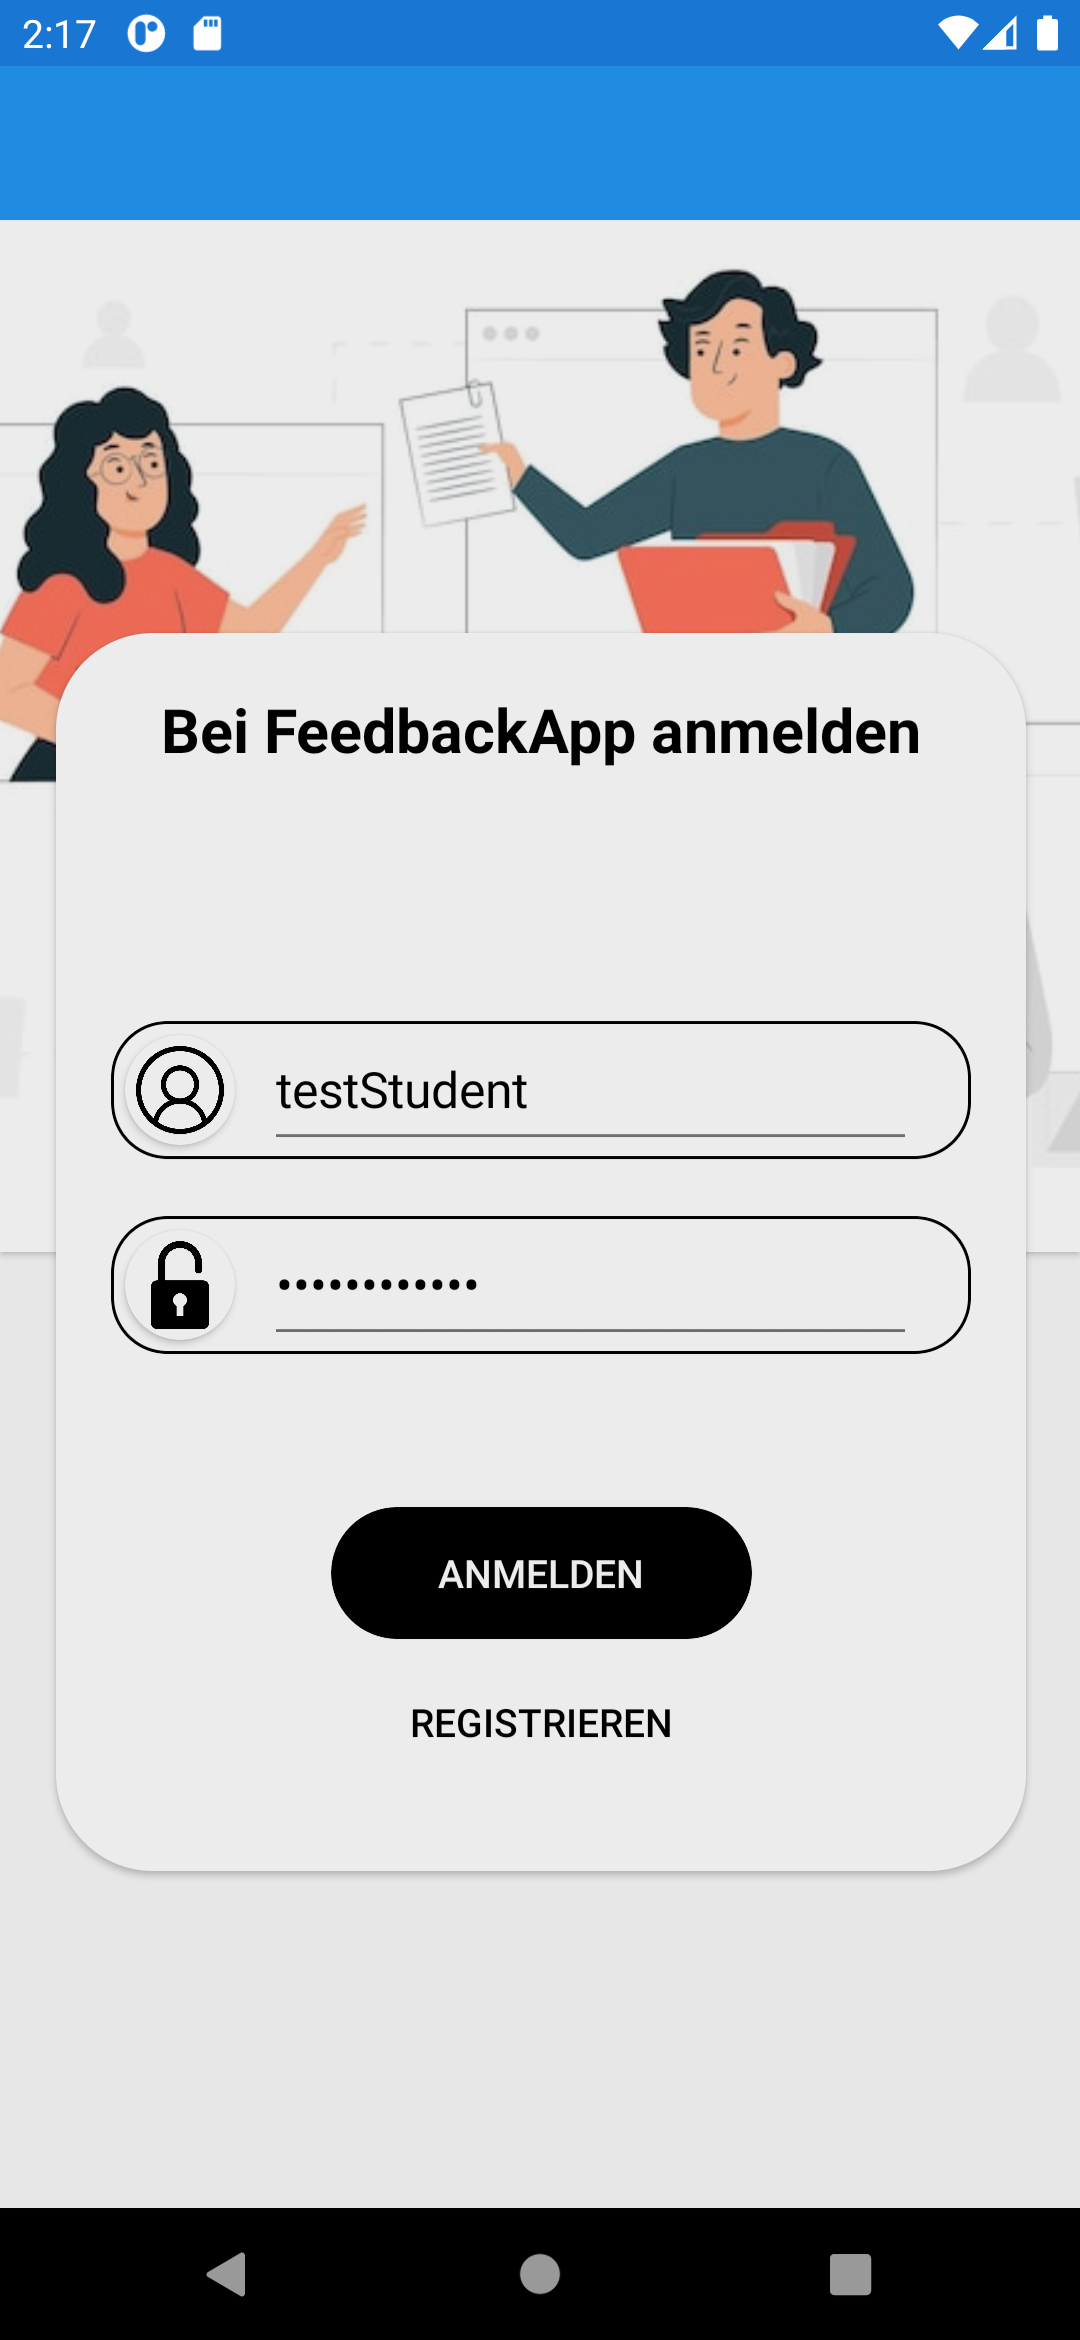
\includegraphics[width=5cm]{pics/Xamarin Student/5 Login Page Full.png}\hfill
    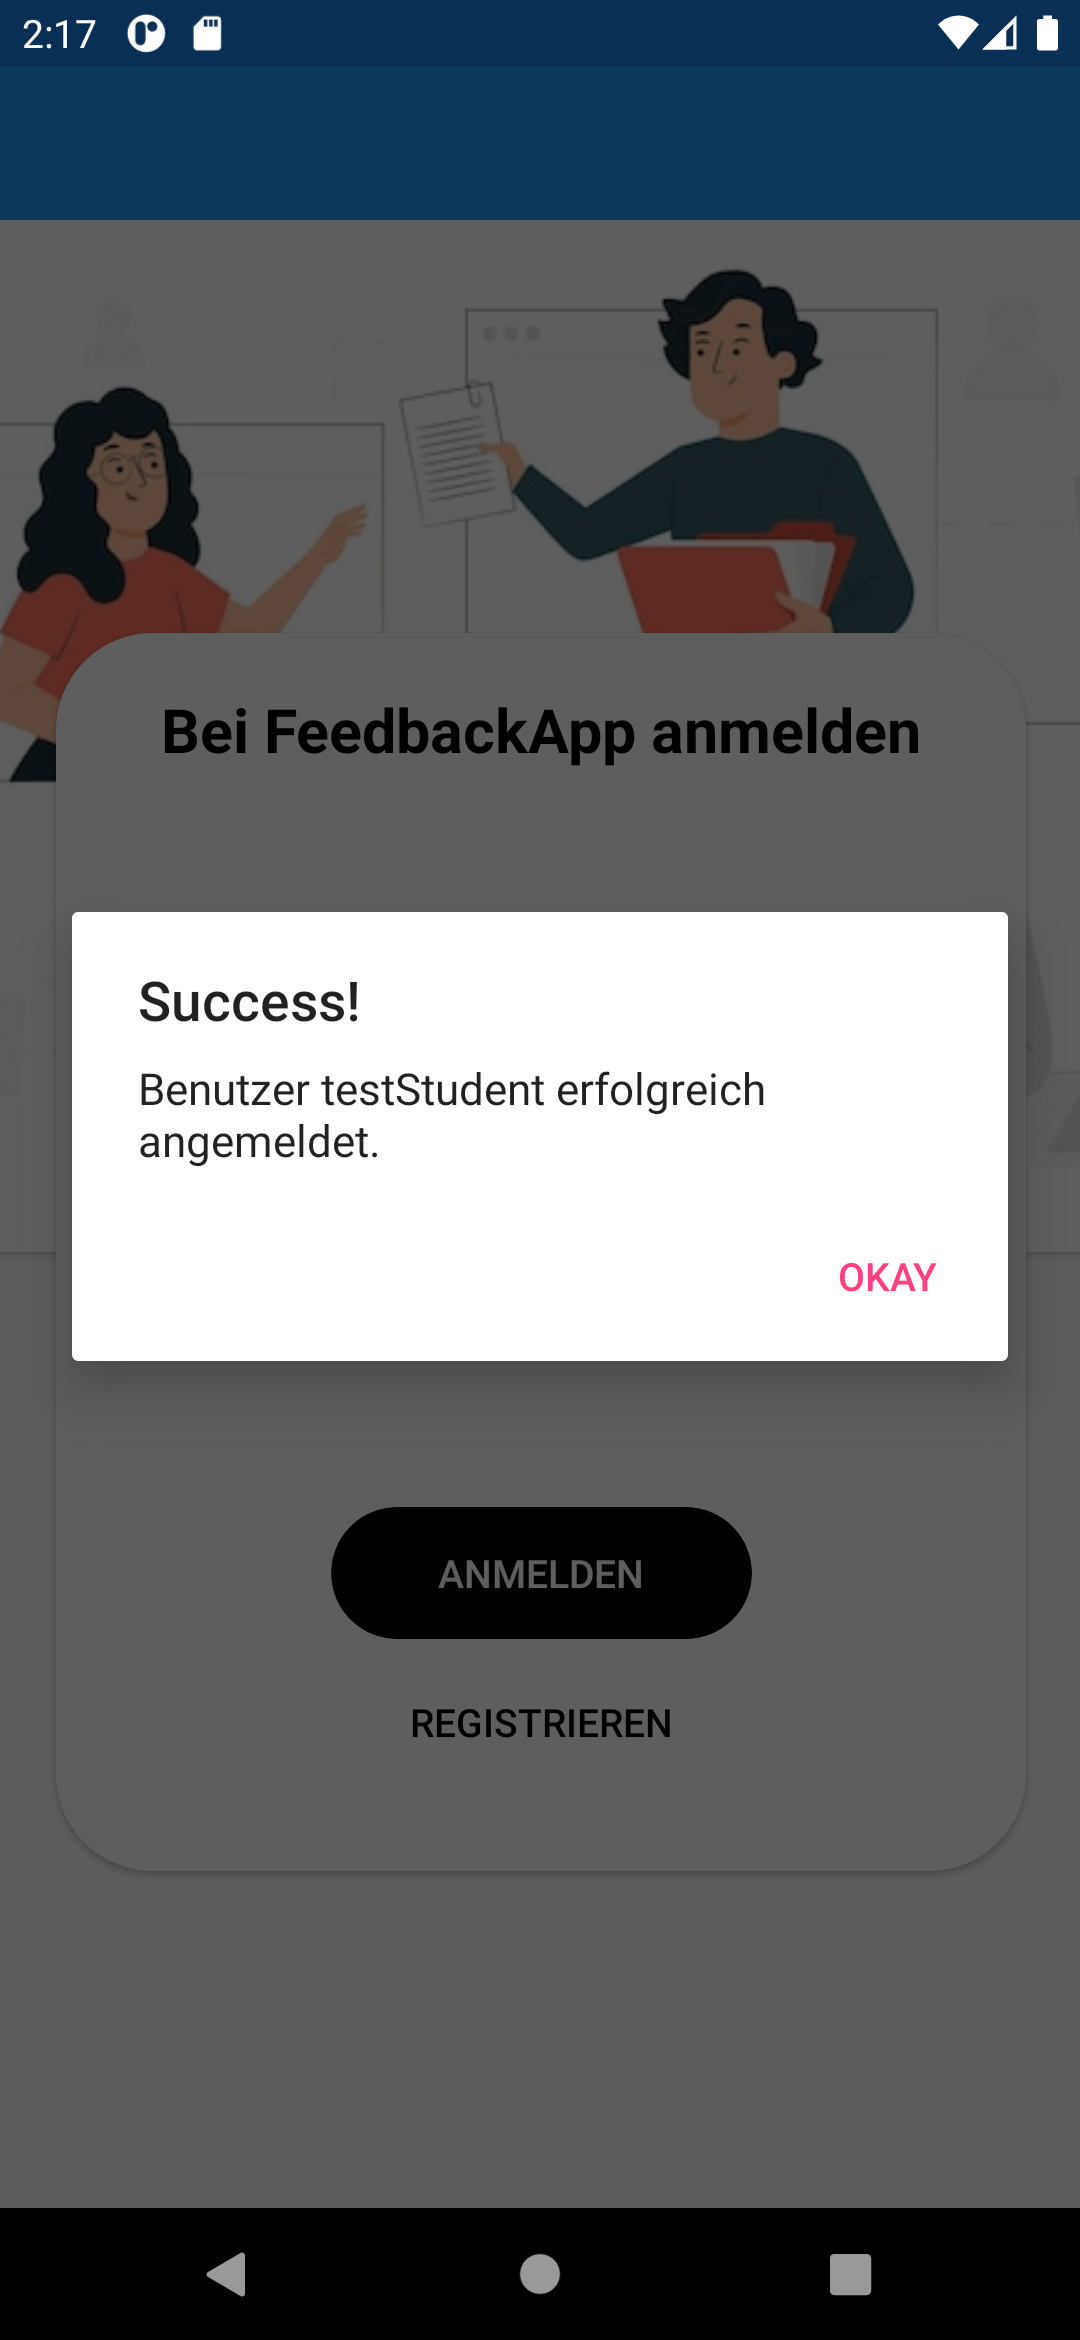
\includegraphics[width=5cm]{pics/Xamarin Student/6 Login Page Success.png}
    \caption[LoginPage]{Login Daten einfügen}
    \end{center}
\end{figure}
Durch die Eingabe von Benutzername und Passwort prüfen wir, ob bereits ein Account eingerichtet ist. Wenn das Konto bereits existiert, erhalten wir eine positive Antwort, andernfalls erhalten wir einen Fehler ("error"). Die Anmeldung ist für Schüler und Lehrer gleich, daher gibt es nur eine Anmeldeschaltfläche für alle Benutzer.\newpage
\newpage

\section{Startseite}
\subsection{Schüler}
Die Startseite für Studierende ist einfach gehalten mit der Hauptfunktion der Fächersuche (Feedbackname). Ganz unten befindet sich ein Button "Feedback geben", der nur aktiviert wird, wenn "Einheit" gefunden wird. In der oberen rechten Ecke befindet sich eine Schaltfläche, die zu den persönlichen Daten des Benutzers führt, wo die Daten angepasst, geändert oder gelöscht werden können. In der Mitte der Seite befindet sich eine Suchmaschine für alle Fächer (Einheit), und der Name muss genau eingegeben werden, um die richtigen Ergebnisse zurückzugeben.
\begin{figure}[h]
    \begin{center}
        \includegraphics*[width=5cm]{pics/Xamarin Student/7 HomePage Student.png}
        \caption[HomePage]{HomePage Student Ansicht}
    \end{center}
\end{figure}
\newpage
Zunächst muss der richtige Name des Themas oder zumindest der richtige Anfangsteil eingegeben werden, und nach der Suchmaschine erhalten wir korrekte Ergebnisse.
\begin{figure}[h]
    \begin{center}
    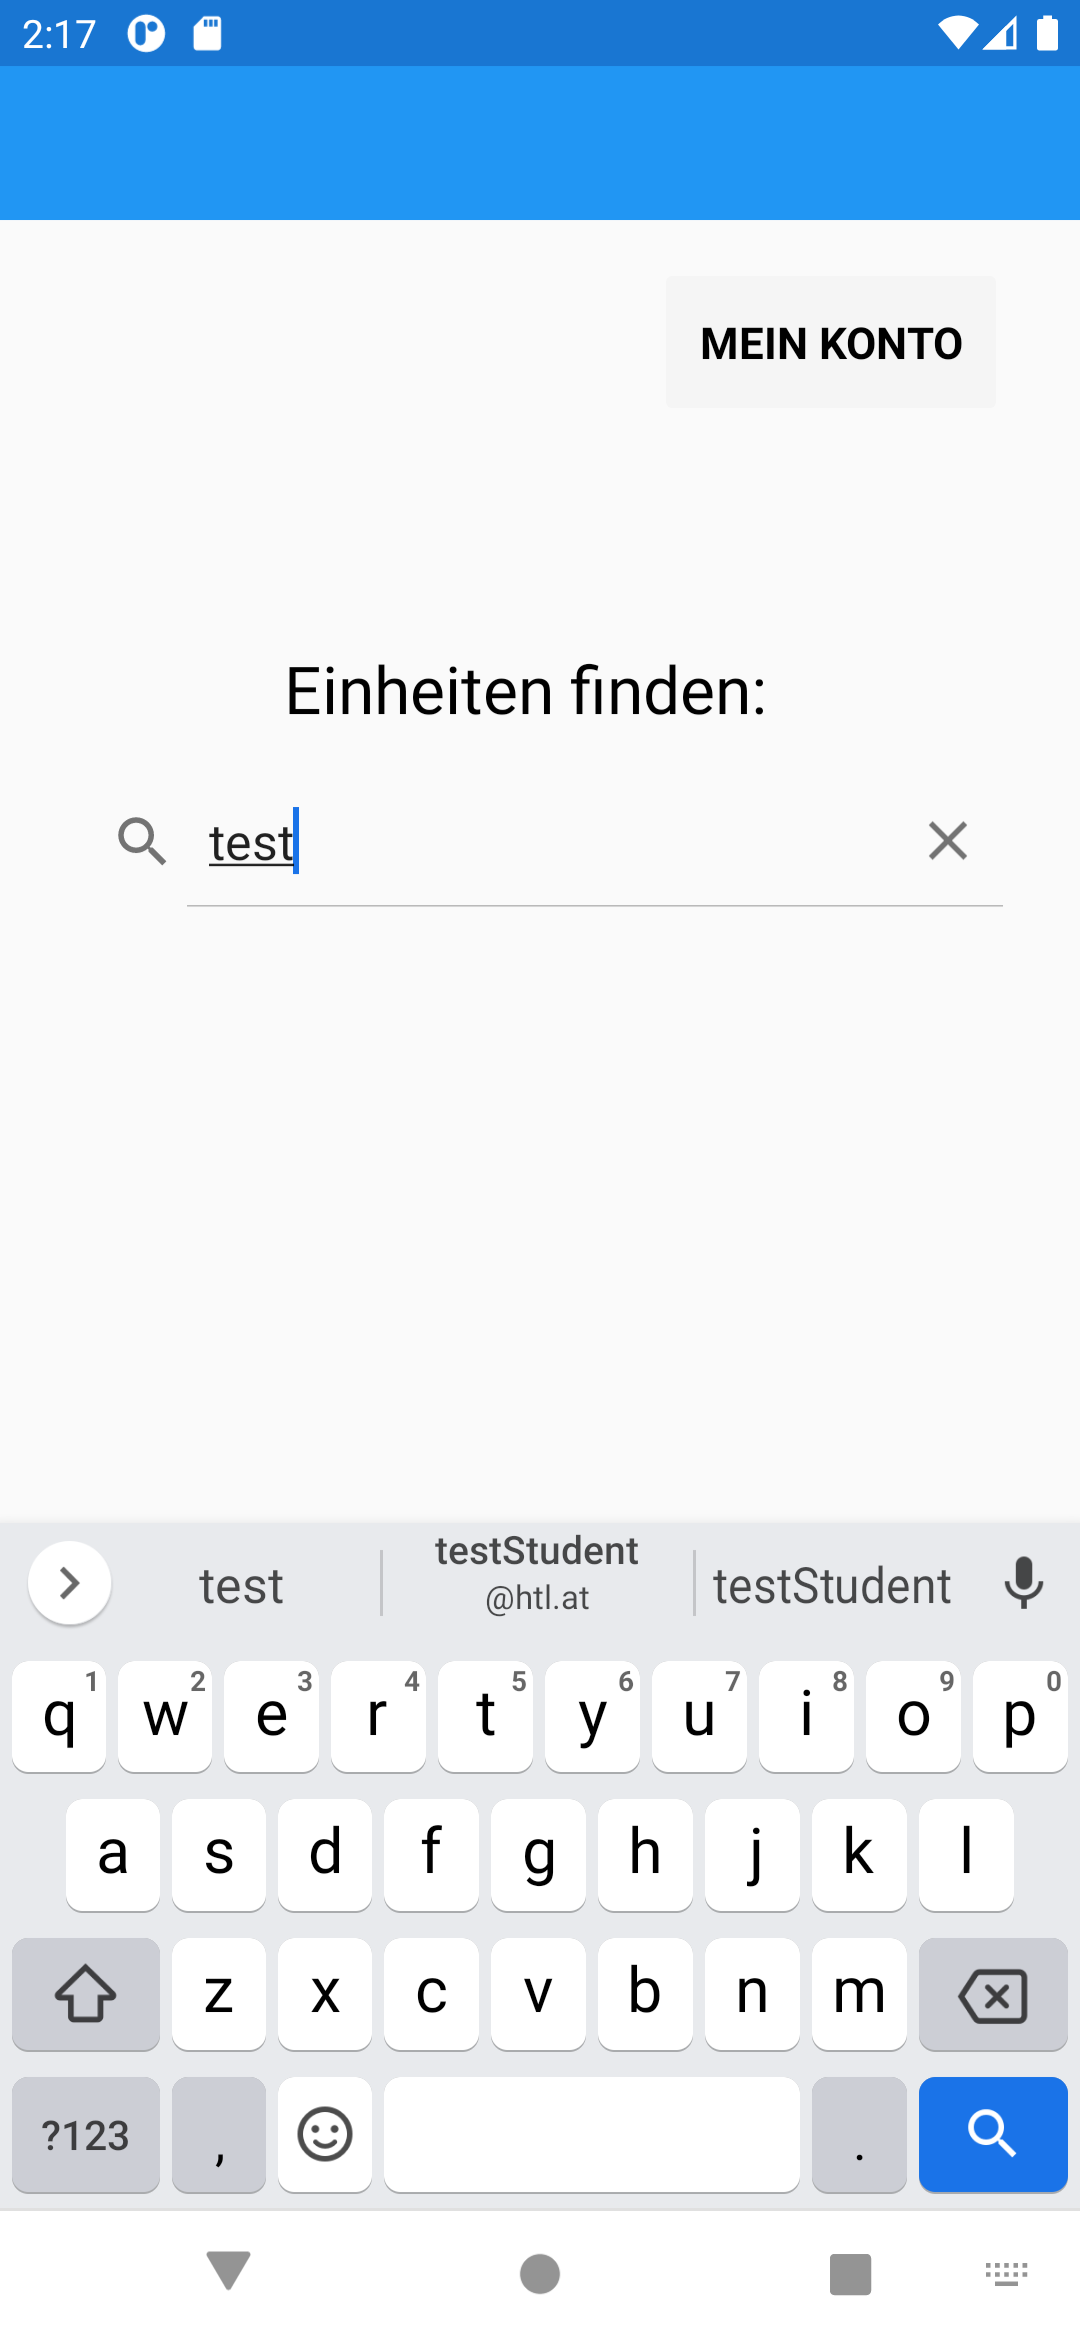
\includegraphics[width=4cm]{pics/Xamarin Student/8 Einheit finden.png}\hfill
    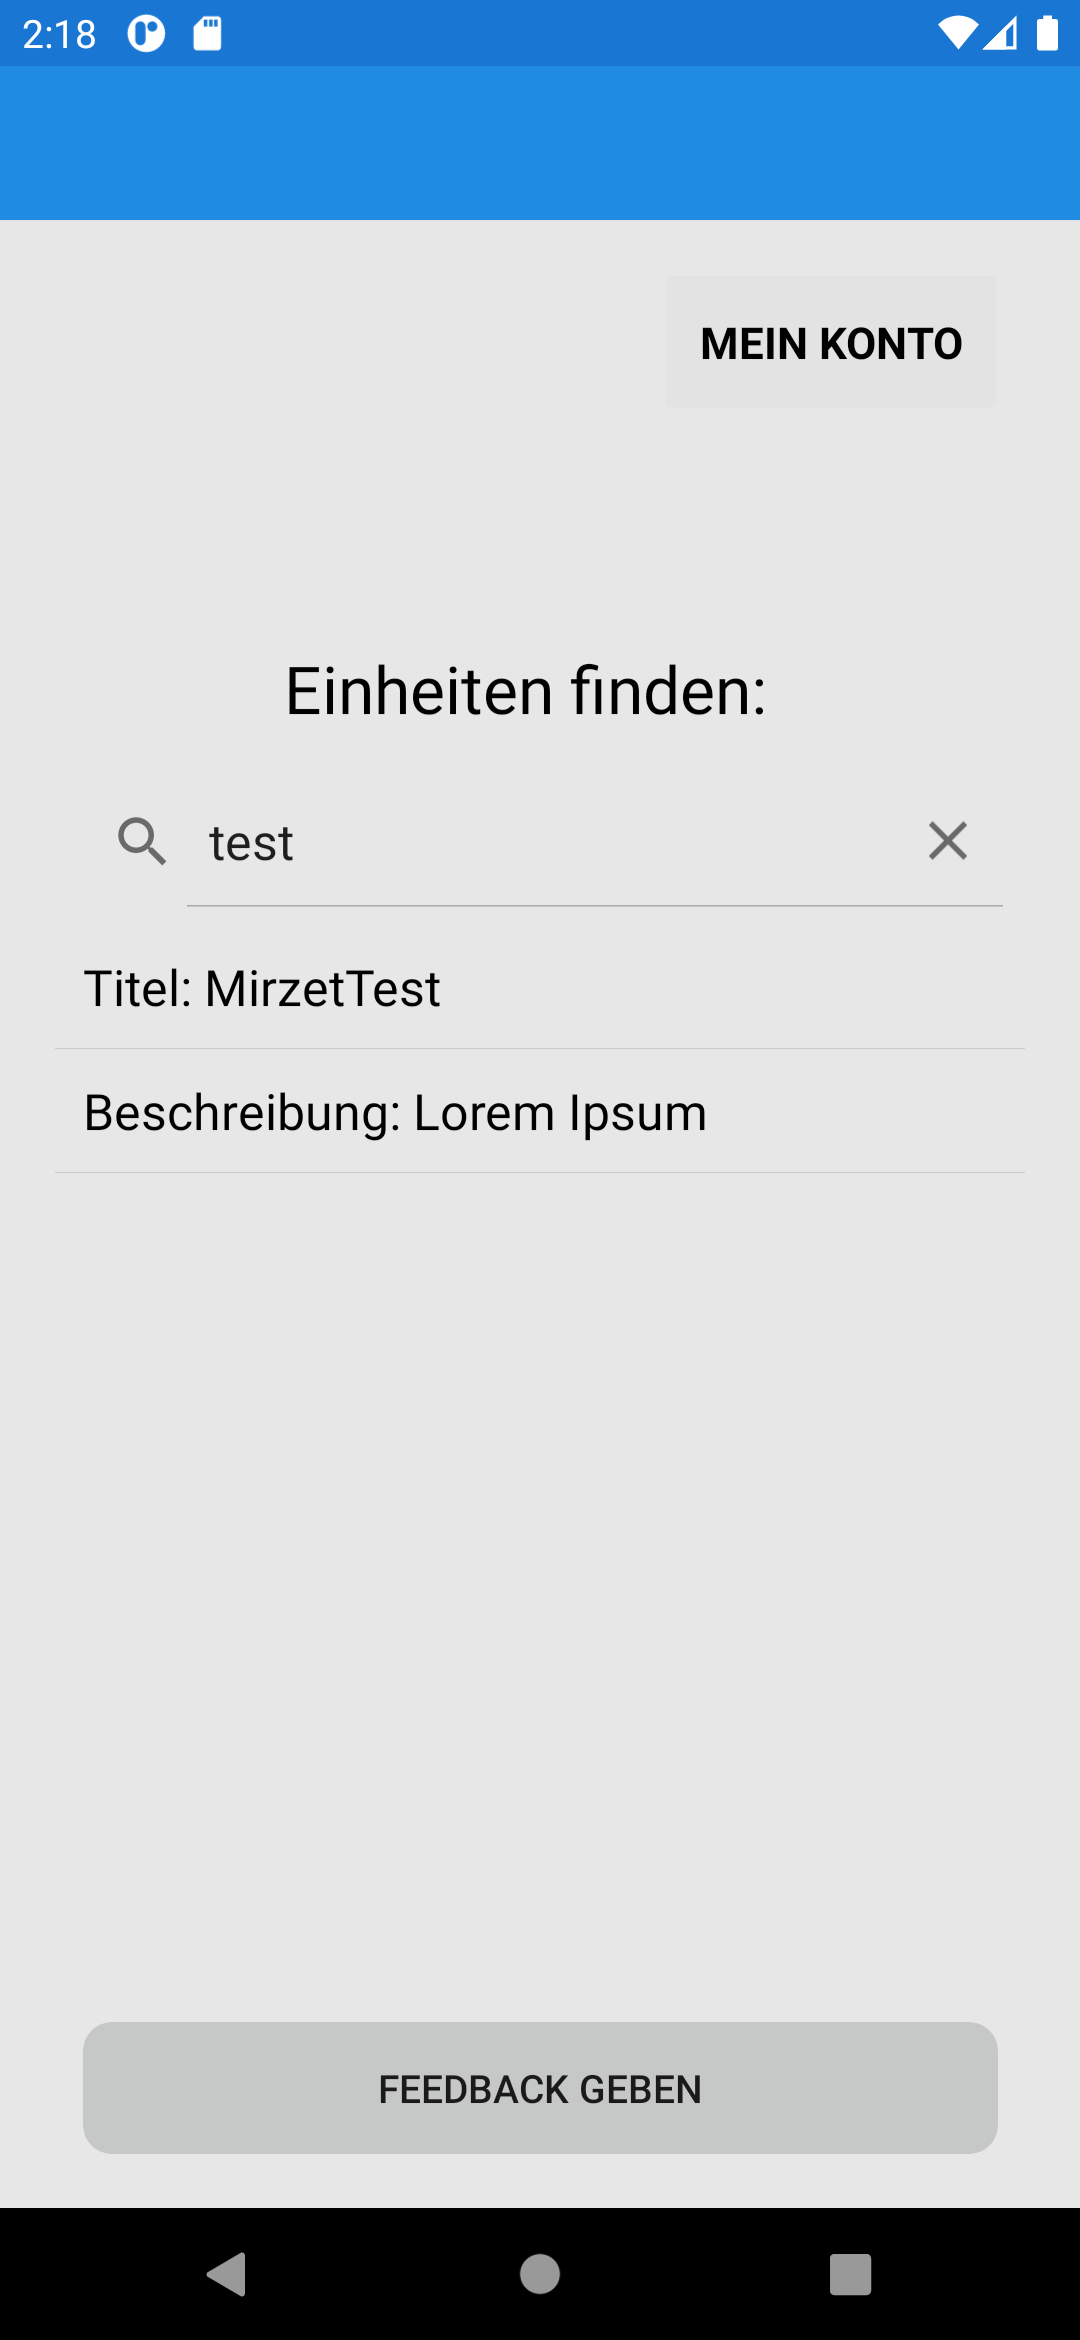
\includegraphics[width=4cm]{pics/Xamarin Student/9 Einheit gefunden.png}
    \caption[HomePage]{Einheiten Ansicht}
    \end{center}
\end{figure}
\newpage

Nachdem der Artikel gefunden wurde, wird die Schaltfläche unten auf der Seite sichtbar und aktiv, und wir können darauf klicken, wenn wir Feedback oder einen Kommentar hinterlassen möchten.
\begin{figure}[h]
    \begin{center}
    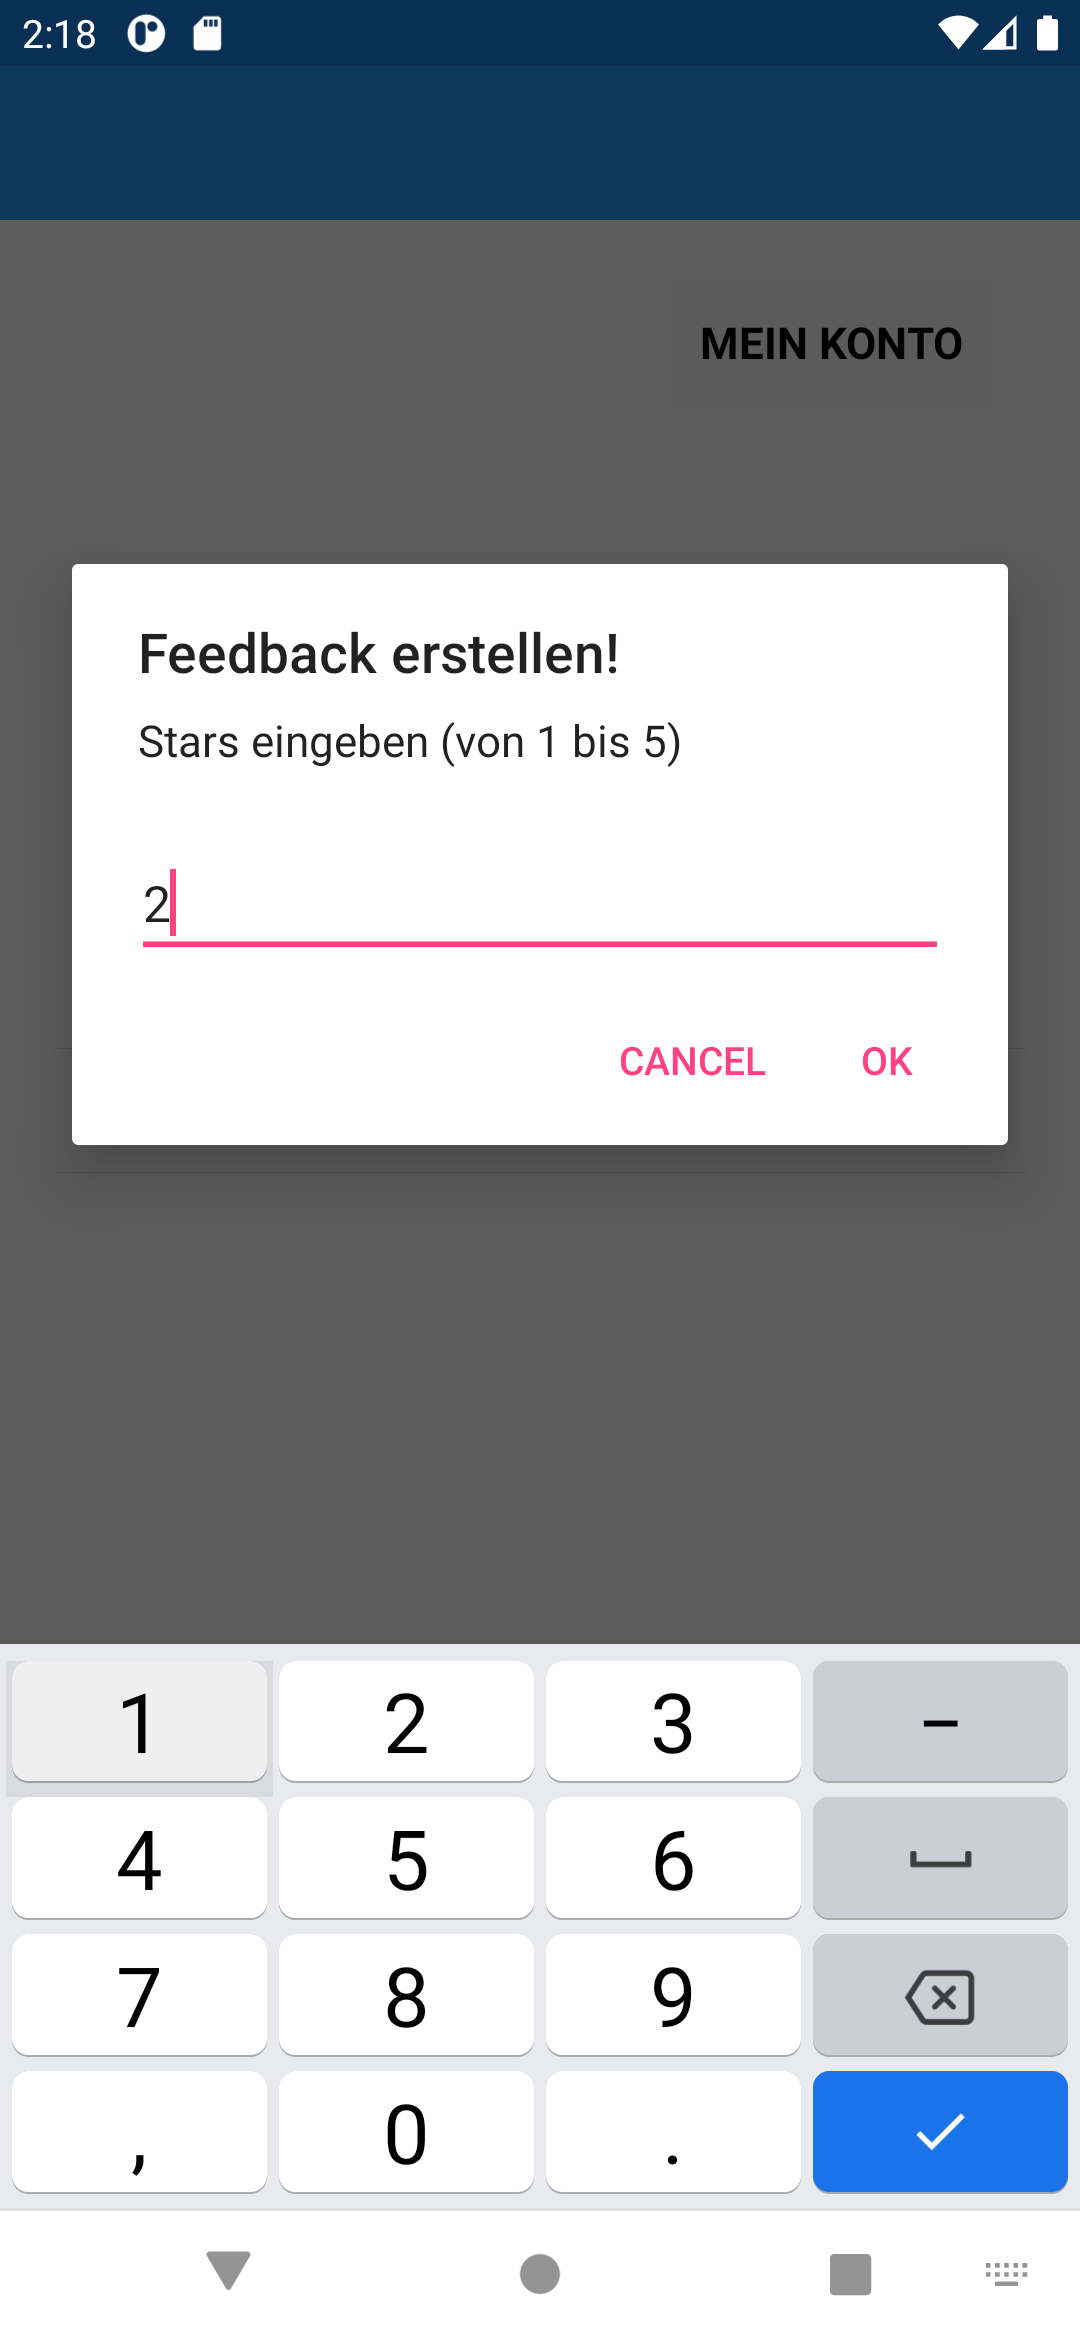
\includegraphics[width=4cm]{pics/Xamarin Student/10 Feedback Star.png}\hfill
    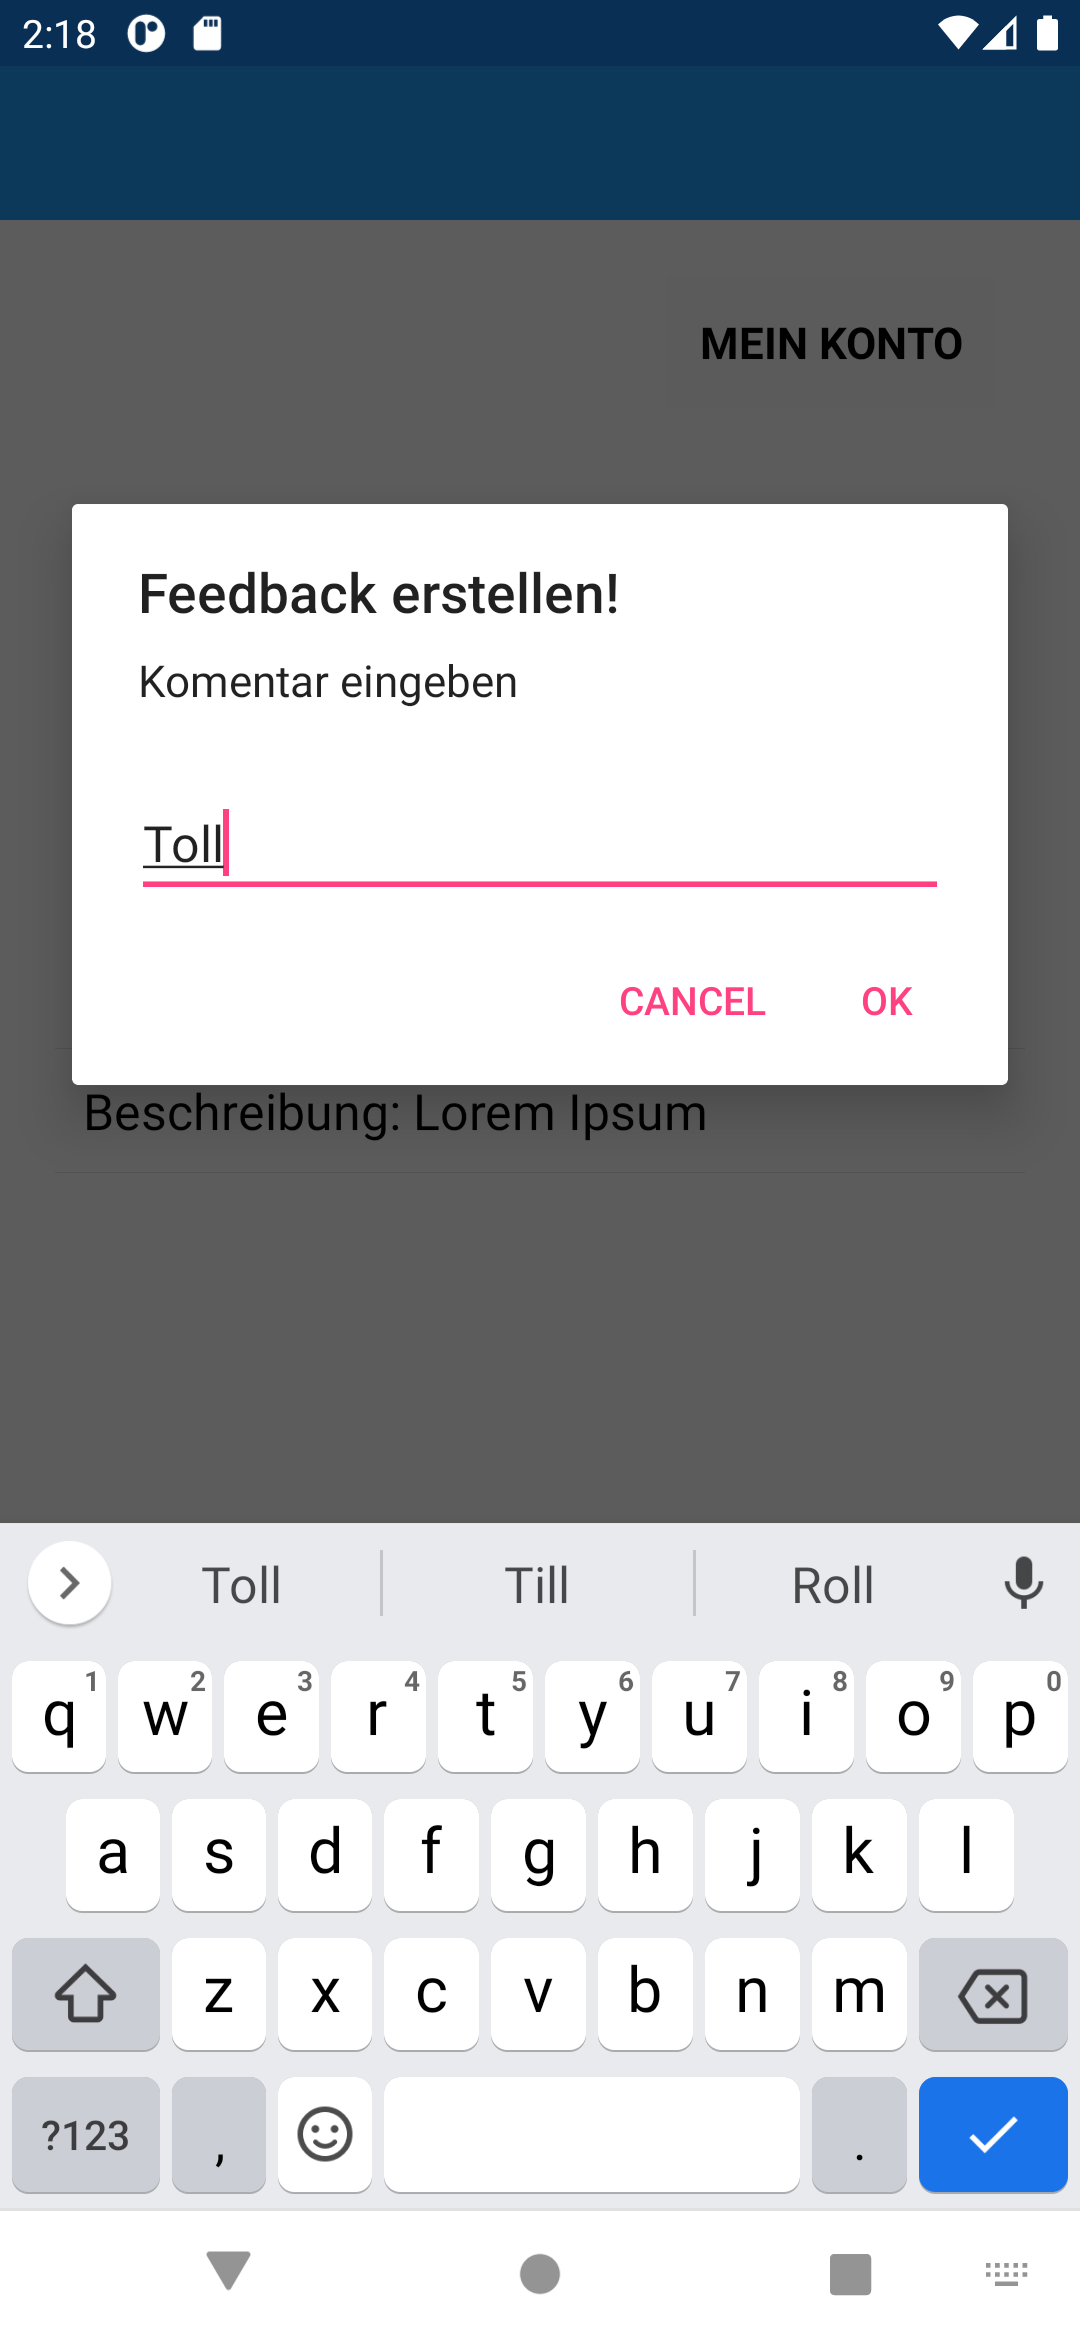
\includegraphics[width=4cm]{pics/Xamarin Student/11 Feedback comm.png}\hfill
    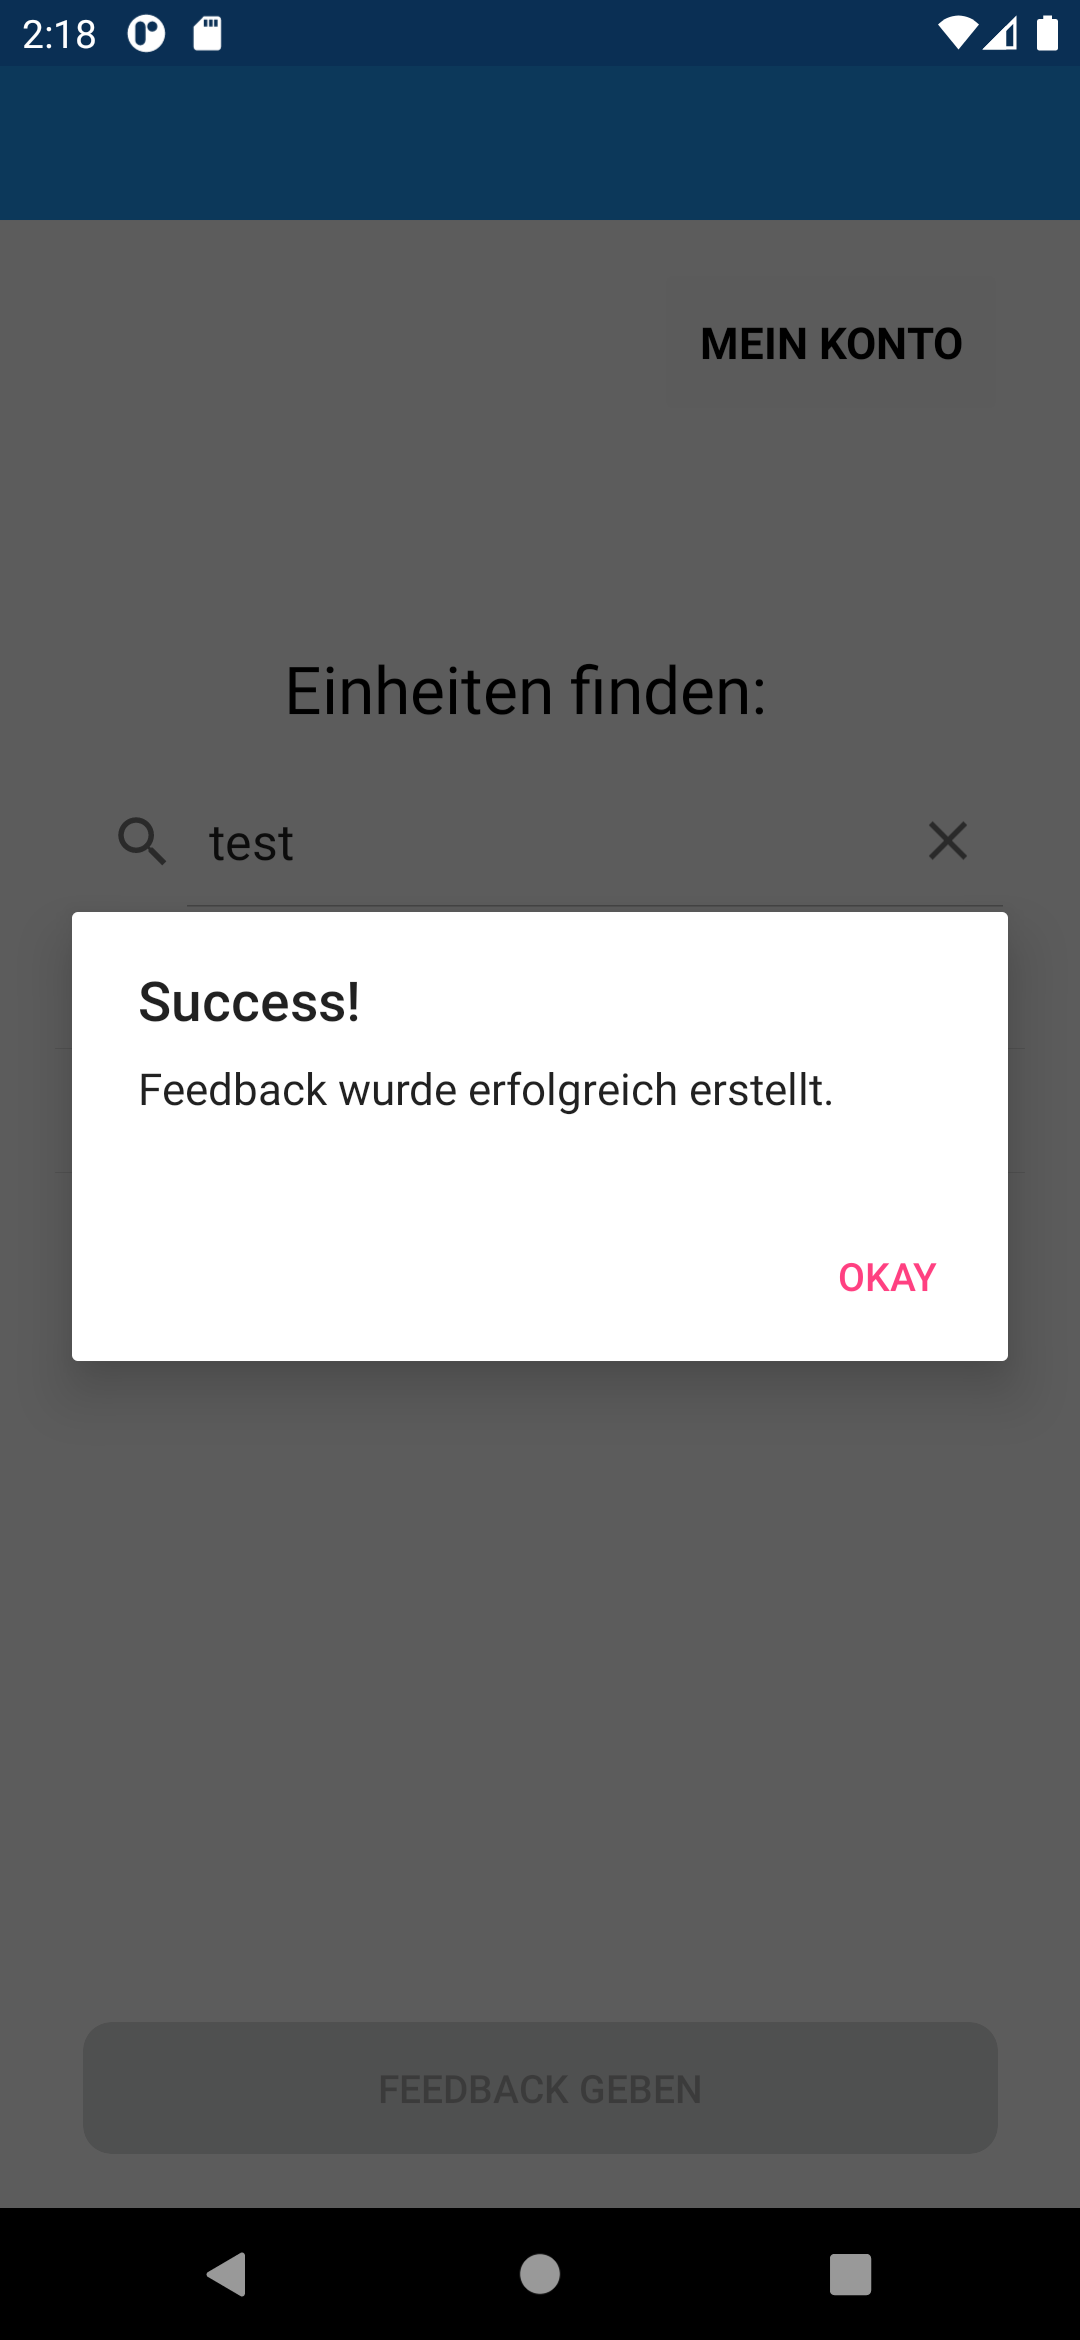
\includegraphics[width=4cm]{pics/Xamarin Student/12 Feedback success.png}
    \caption[HomePage]{Feedback geben Ansicht}
    \end{center}
\end{figure}
\newline
Wenn wir eine Bewertung über 5 oder unter 1 eingeben, erhalten wir eine Fehlermeldung und das Feedback wird nicht gespeichert.
Nach erfolgreicher Abgabe von Feedback ist der Button „Feedback geben“ wieder inaktiv und wir können es nicht noch einmal geben.
\newpage

\subsection{Lehrer}
Die Startseite für Lehrer ist die gleiche wie für Schüler, nur haben wir zusätzlich einen Button zum Anlegen von Fächern. Darüber hinaus gibt es auch eine Suchmaschine, um zu prüfen, ob der Artikel, den wir eingeben möchten, bereits existiert. Natürlich gibt es auch einen Button für das Benutzerkonto.
\begin{figure}[h]
    \begin{center}
        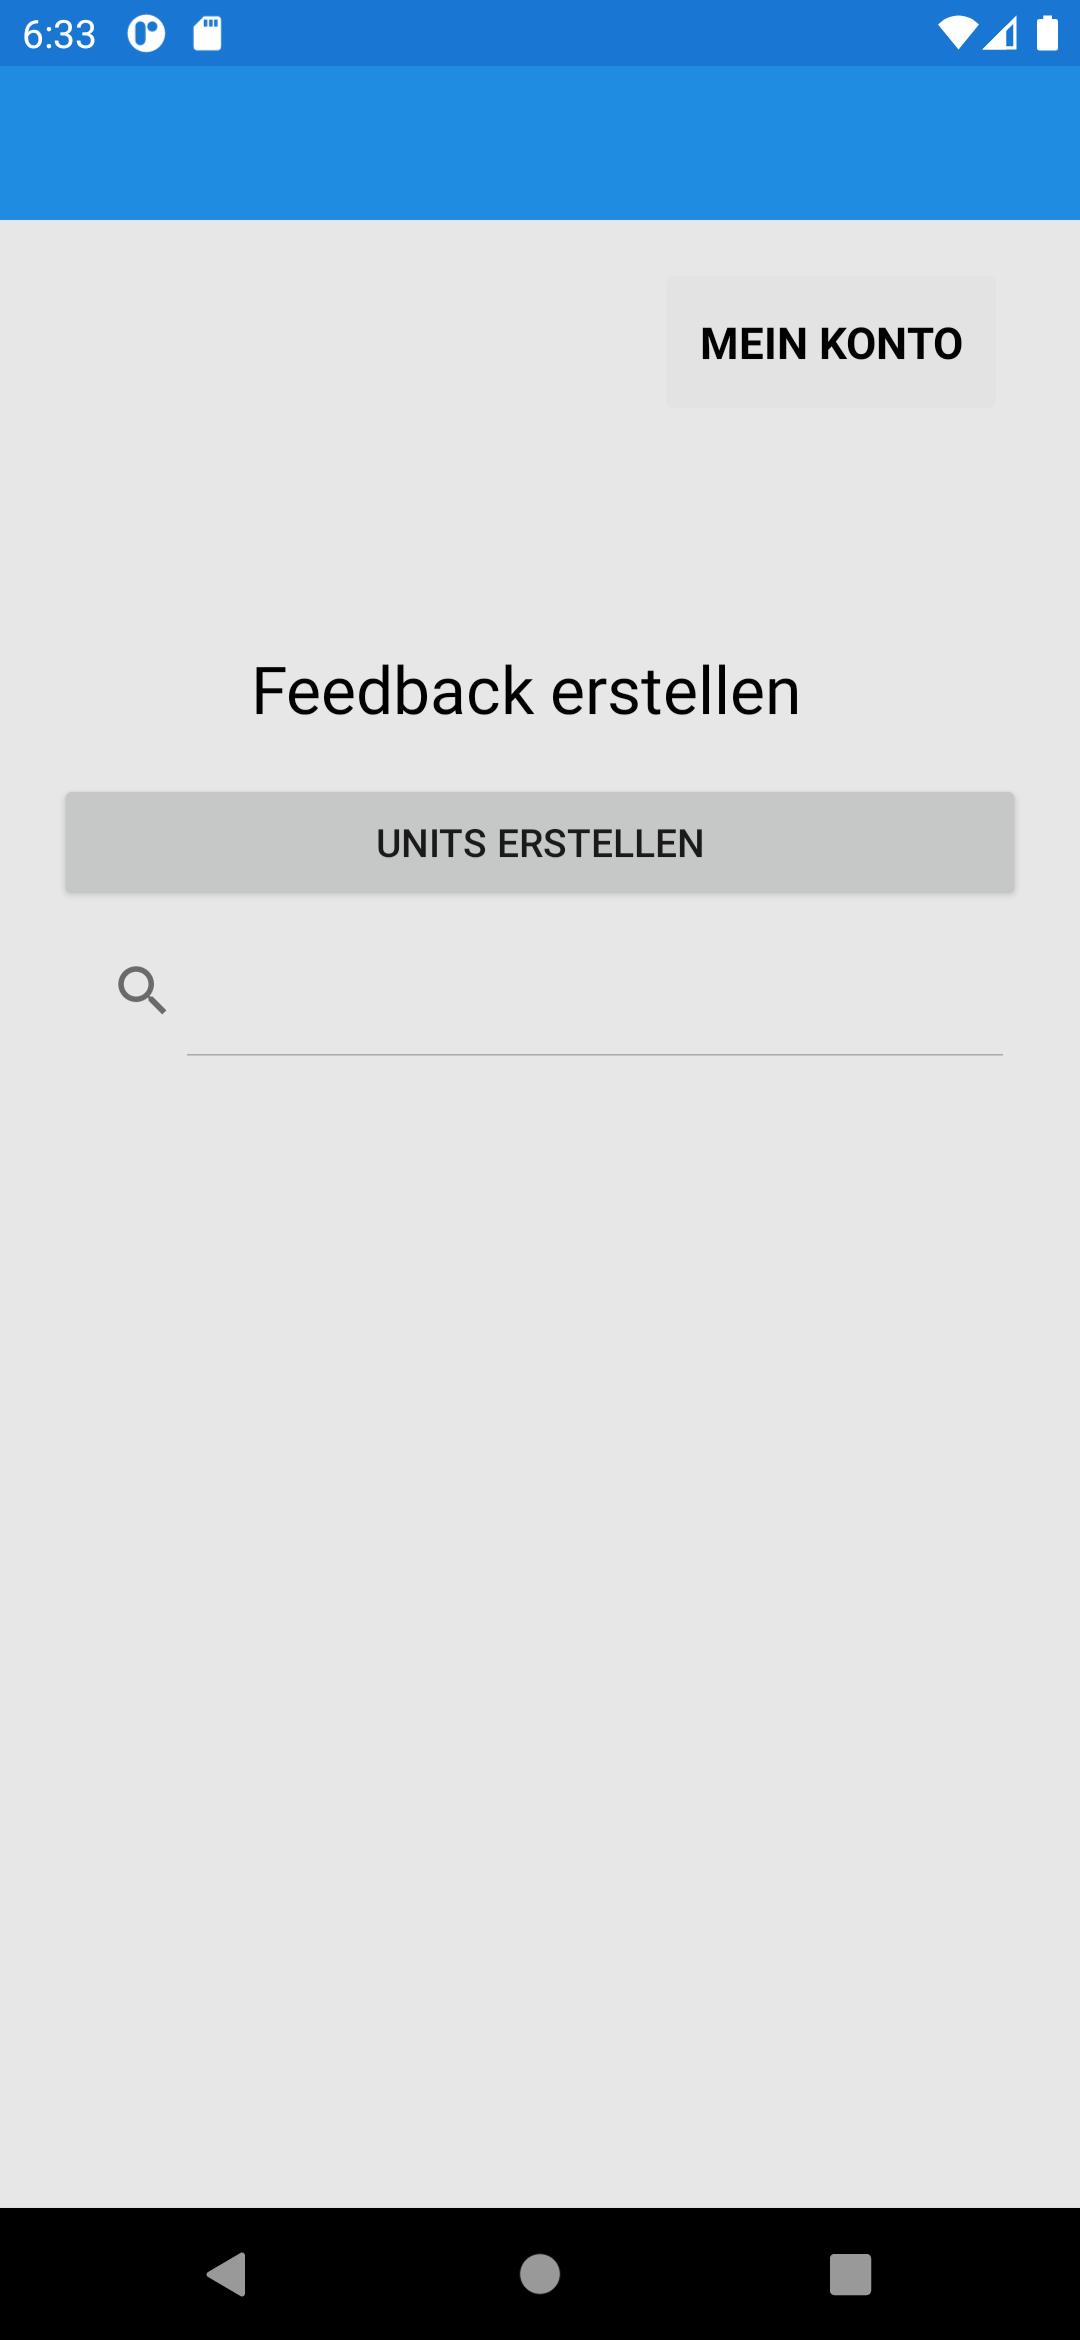
\includegraphics[width=4cm]{pics/Xamarin Lehrer/2 HomePage Lehrer.png}\hfill
        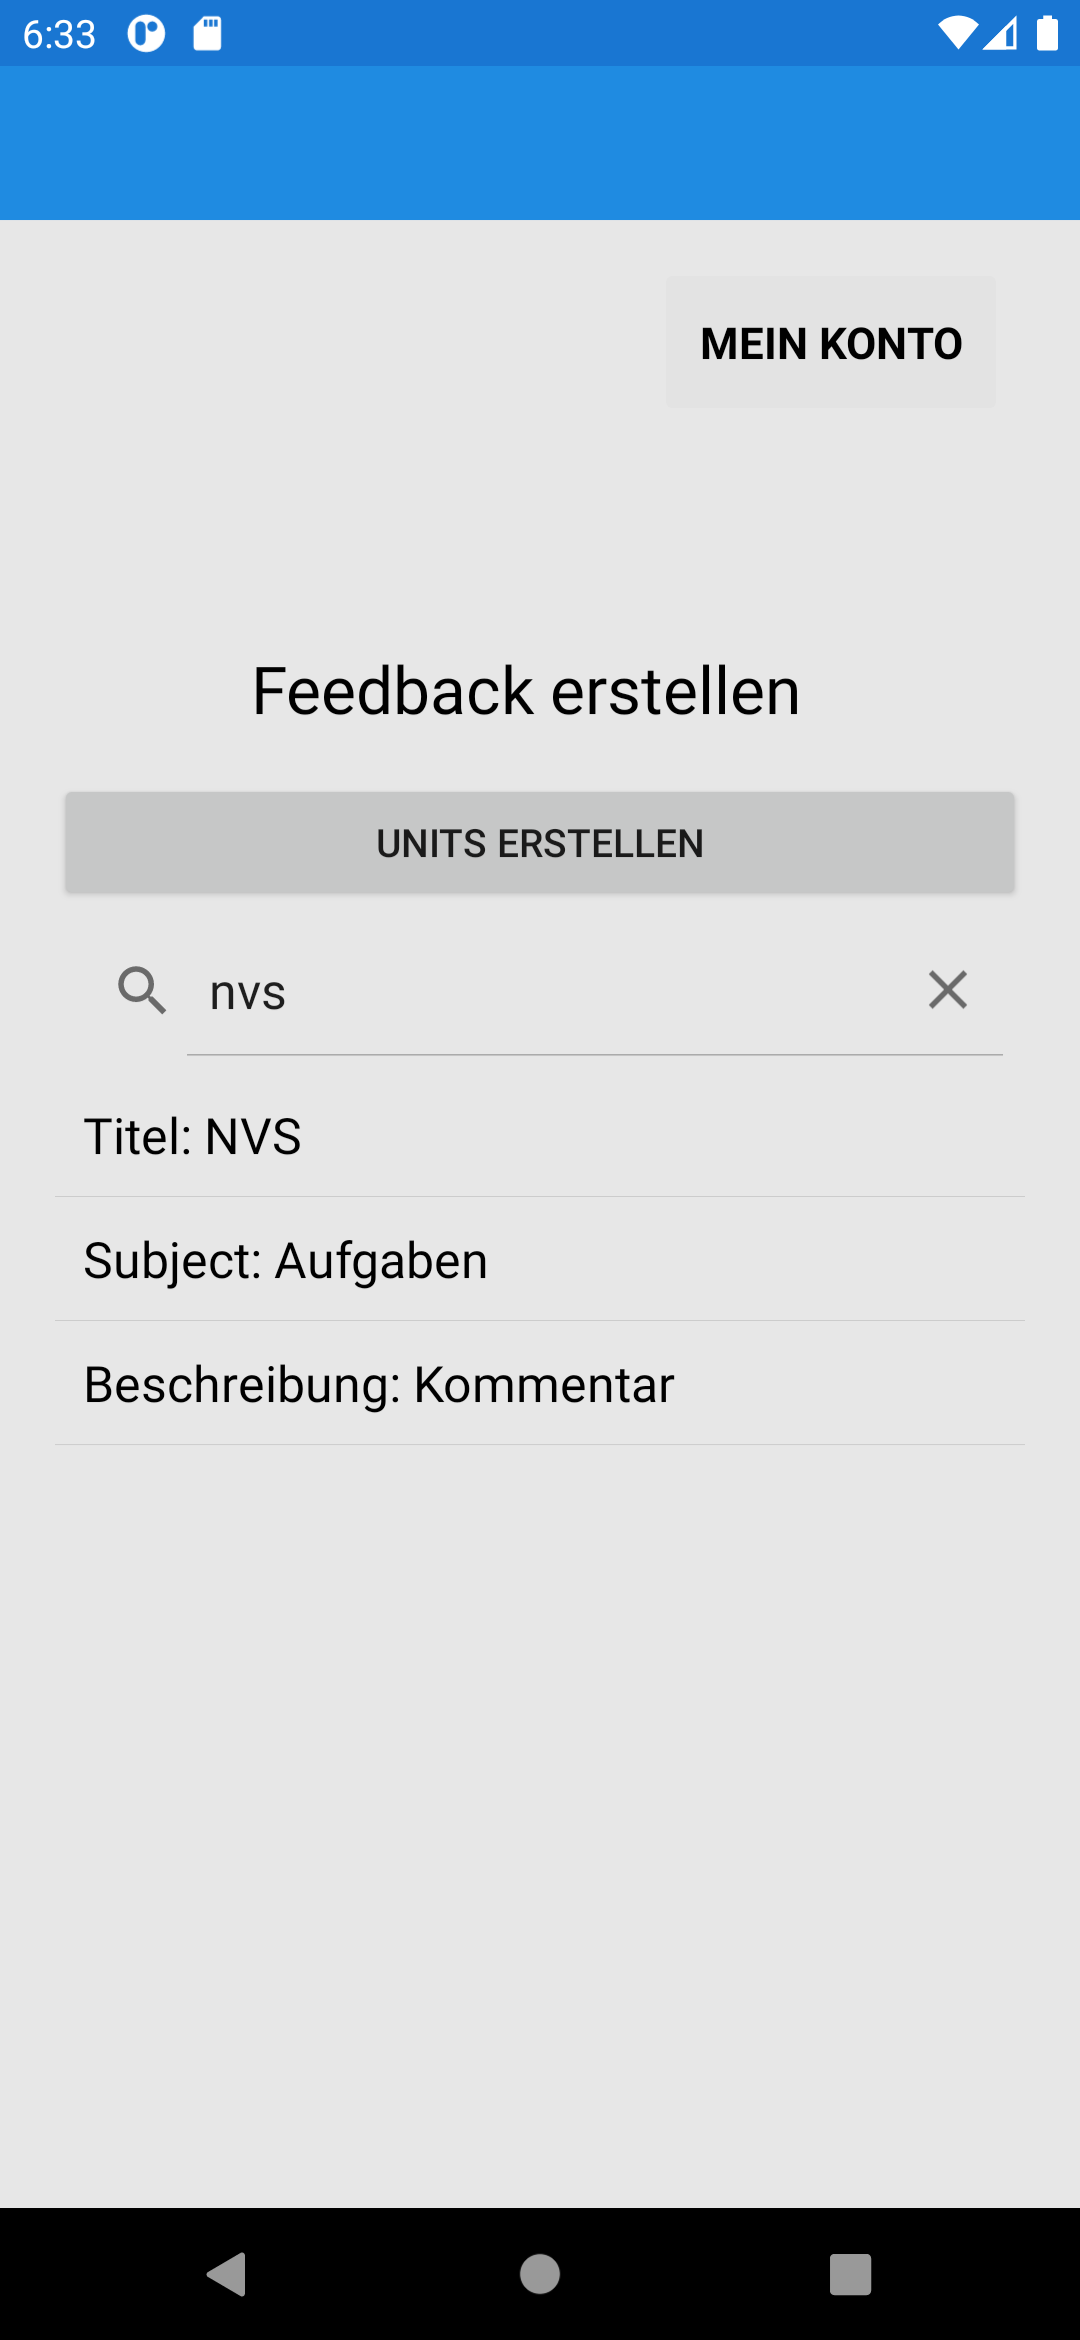
\includegraphics[width=4cm]{pics/Xamarin Lehrer/3 Unit finden.png}
        \caption[HomePage]{HomePage Lehrer Ansicht}
    \end{center}
\end{figure}
\newpage
Um einen neuen Betreff einzugeben, ist die Eingabe von Titel, Betreff und Beschreibung des Betreffs obligatorisch. Das Formular wird in 3 Schritten ausgefüllt, und wenn alles korrekt eingetragen ist, erhalten wir eine positive Antwort.
\begin{figure}[h]
    \begin{center}
        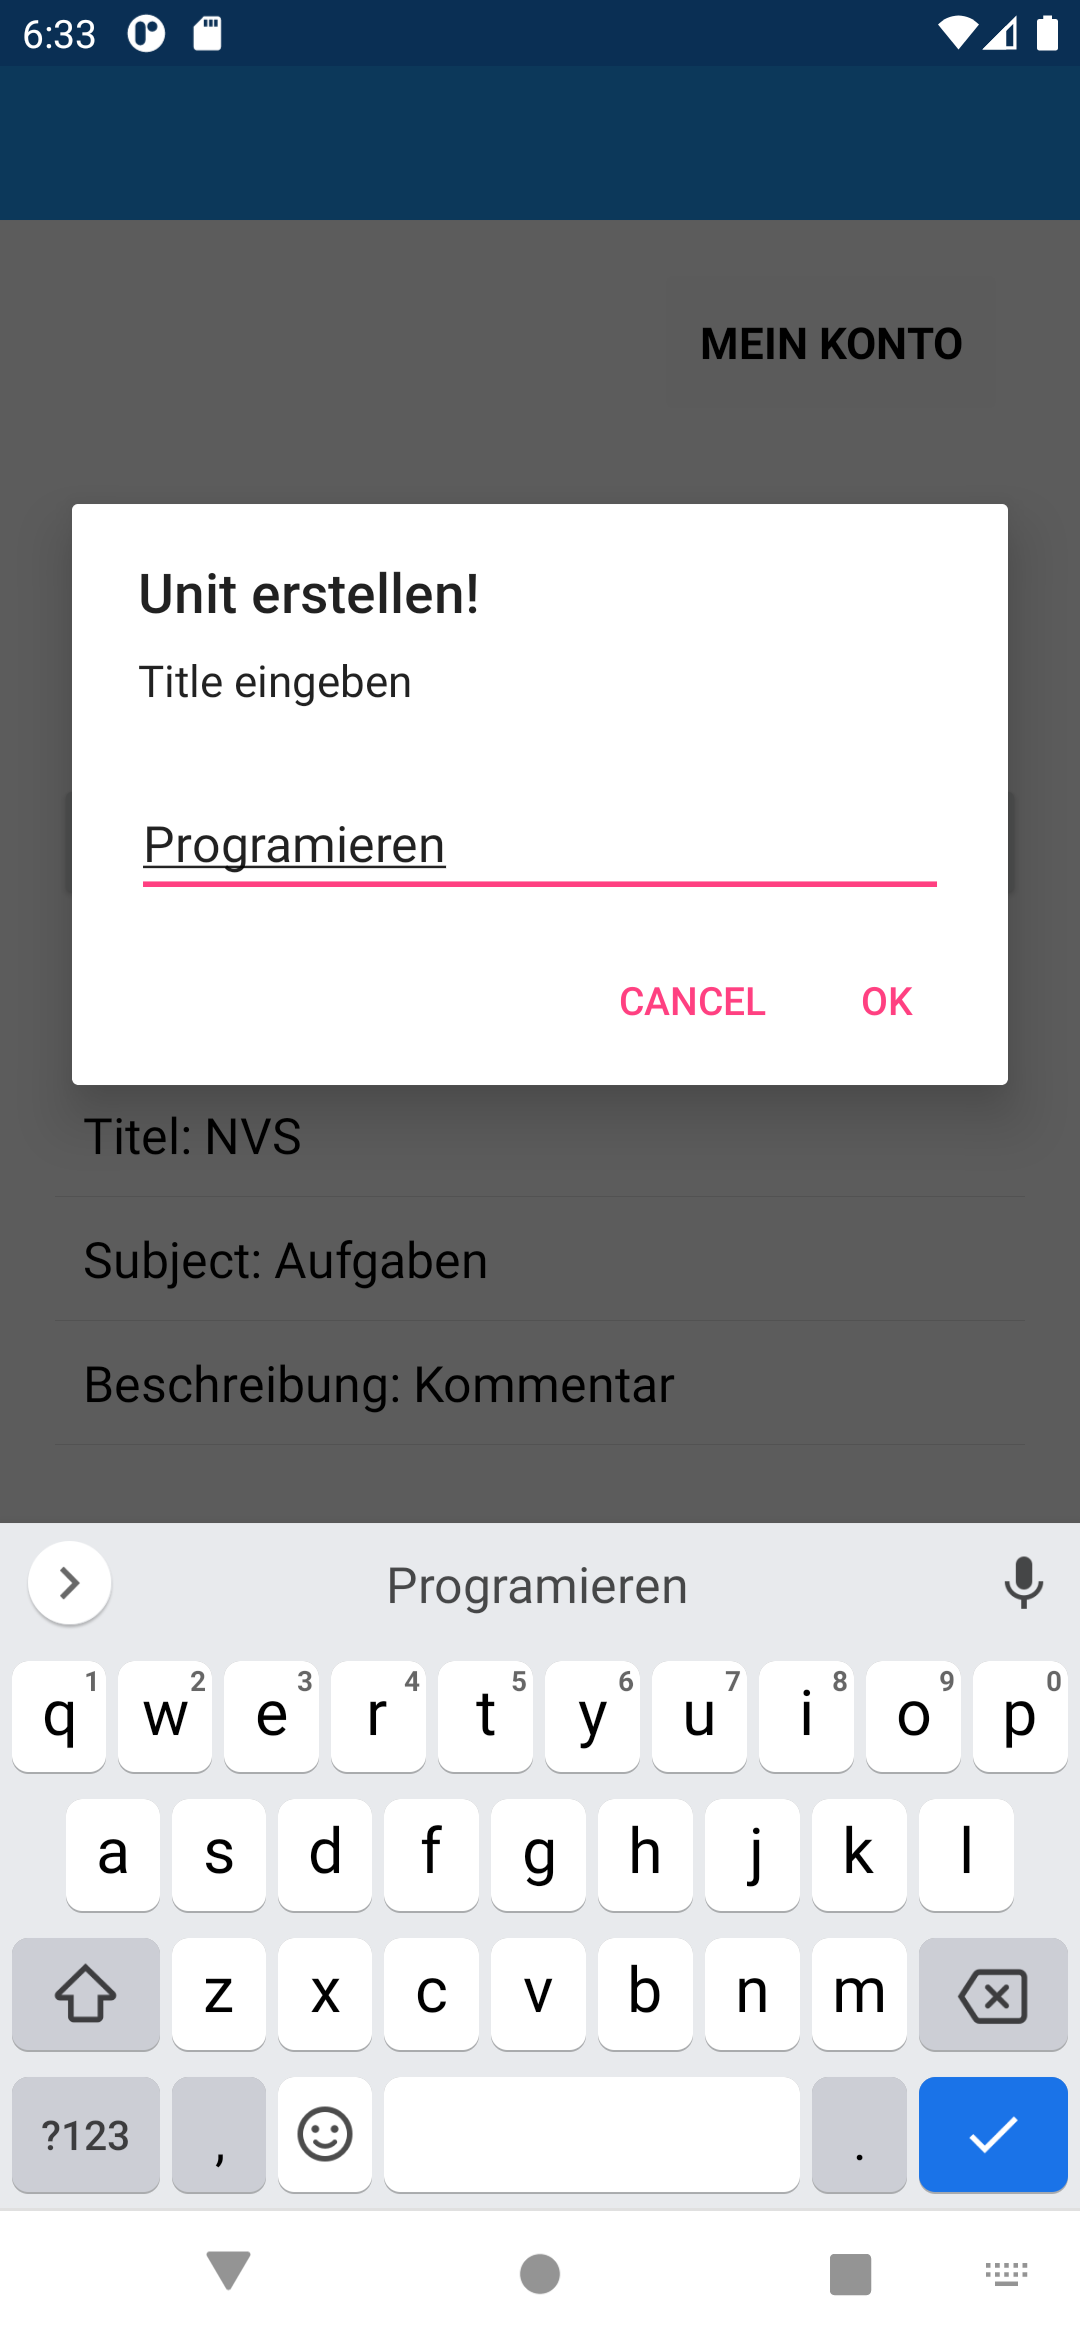
\includegraphics[width=4cm]{pics/Xamarin Lehrer/5.png}\hfill
        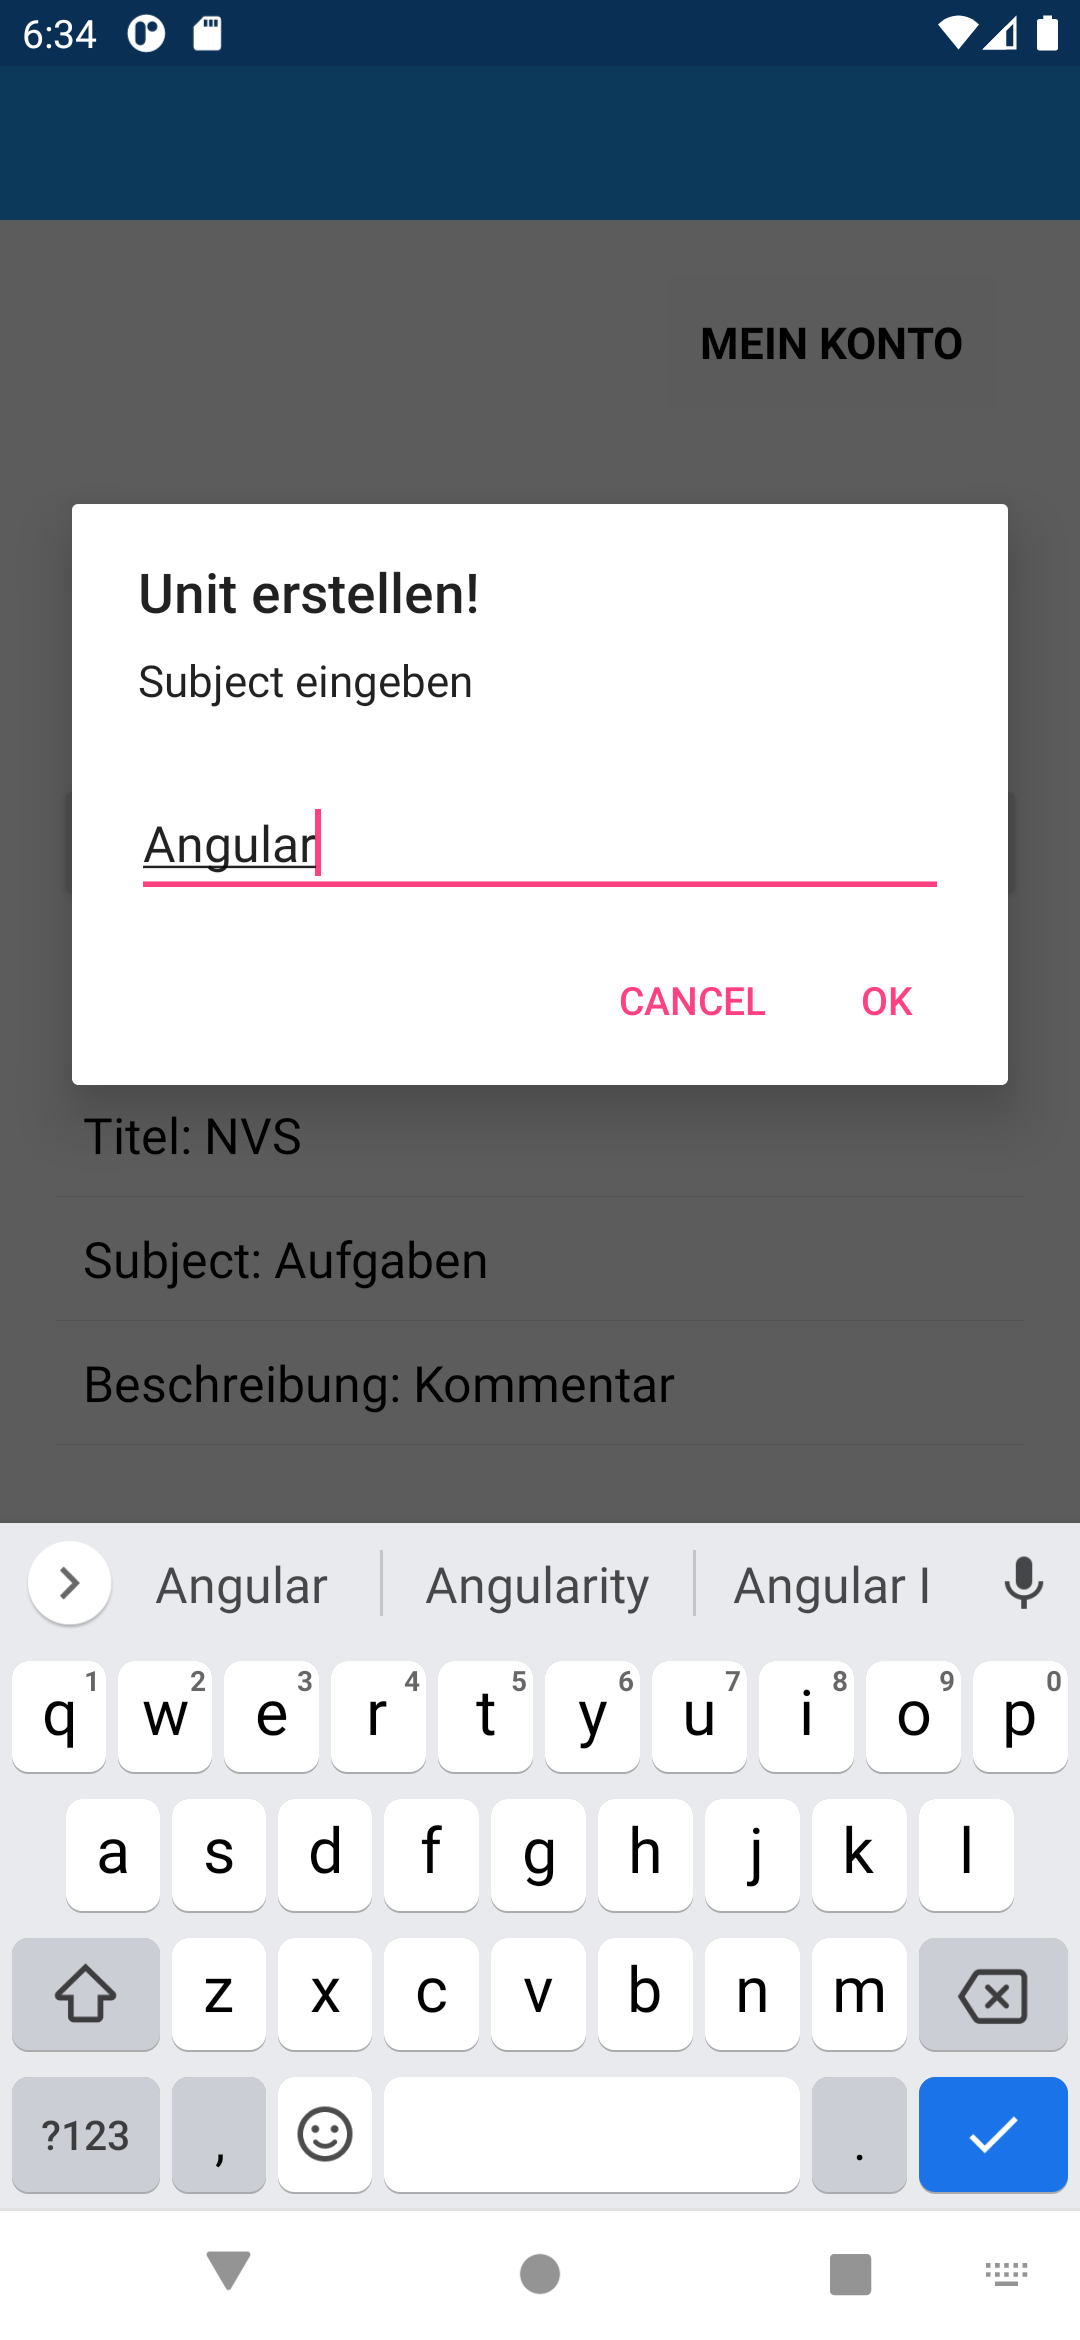
\includegraphics[width=4cm]{pics/Xamarin Lehrer/6.png}
    \end{center}
\end{figure}
\begin{figure}[h]
    \begin{center}
        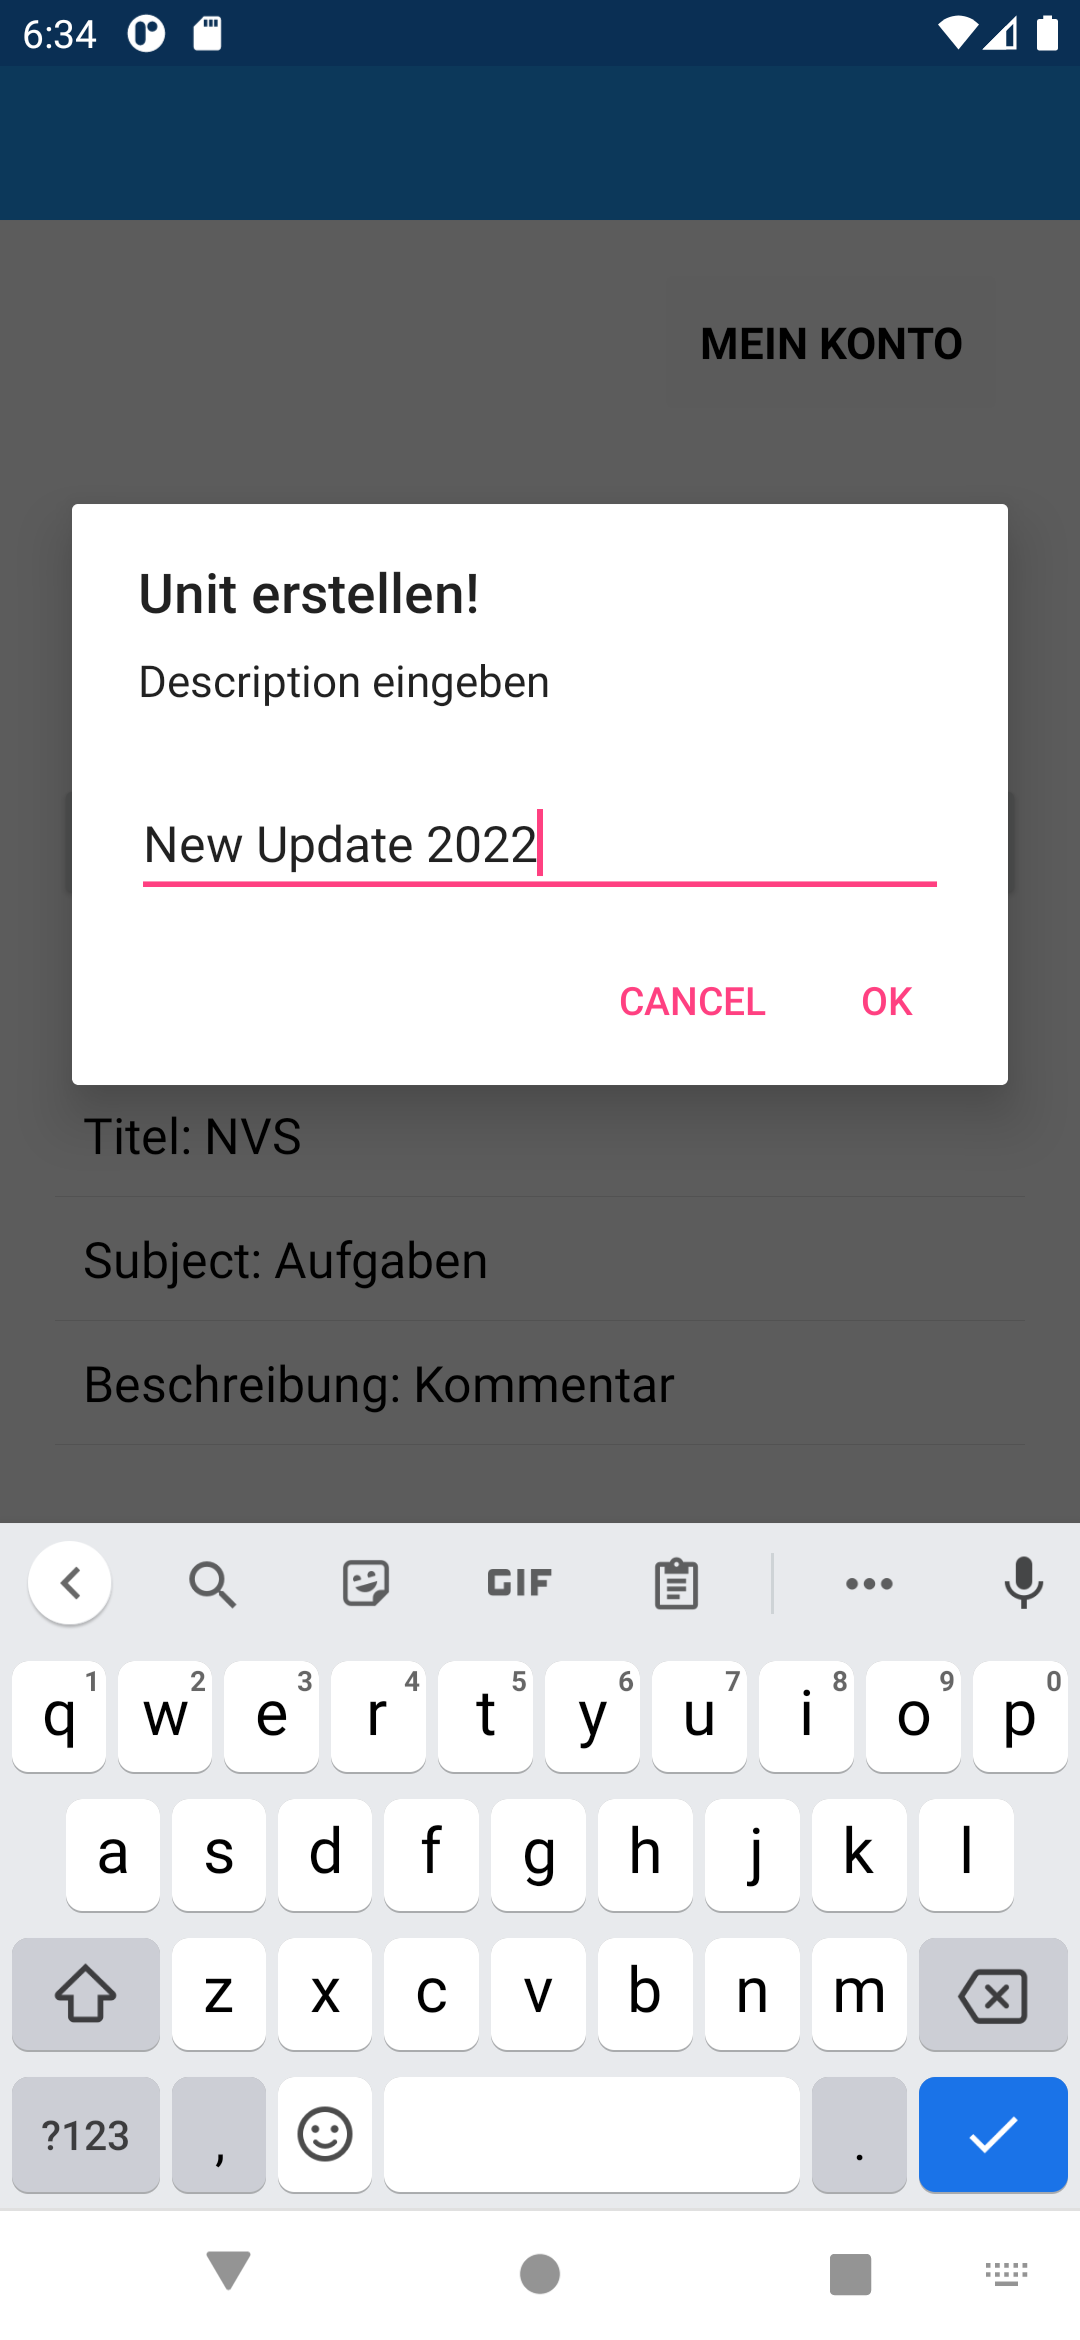
\includegraphics[width=4cm]{pics/Xamarin Lehrer/7.png}\hfill
        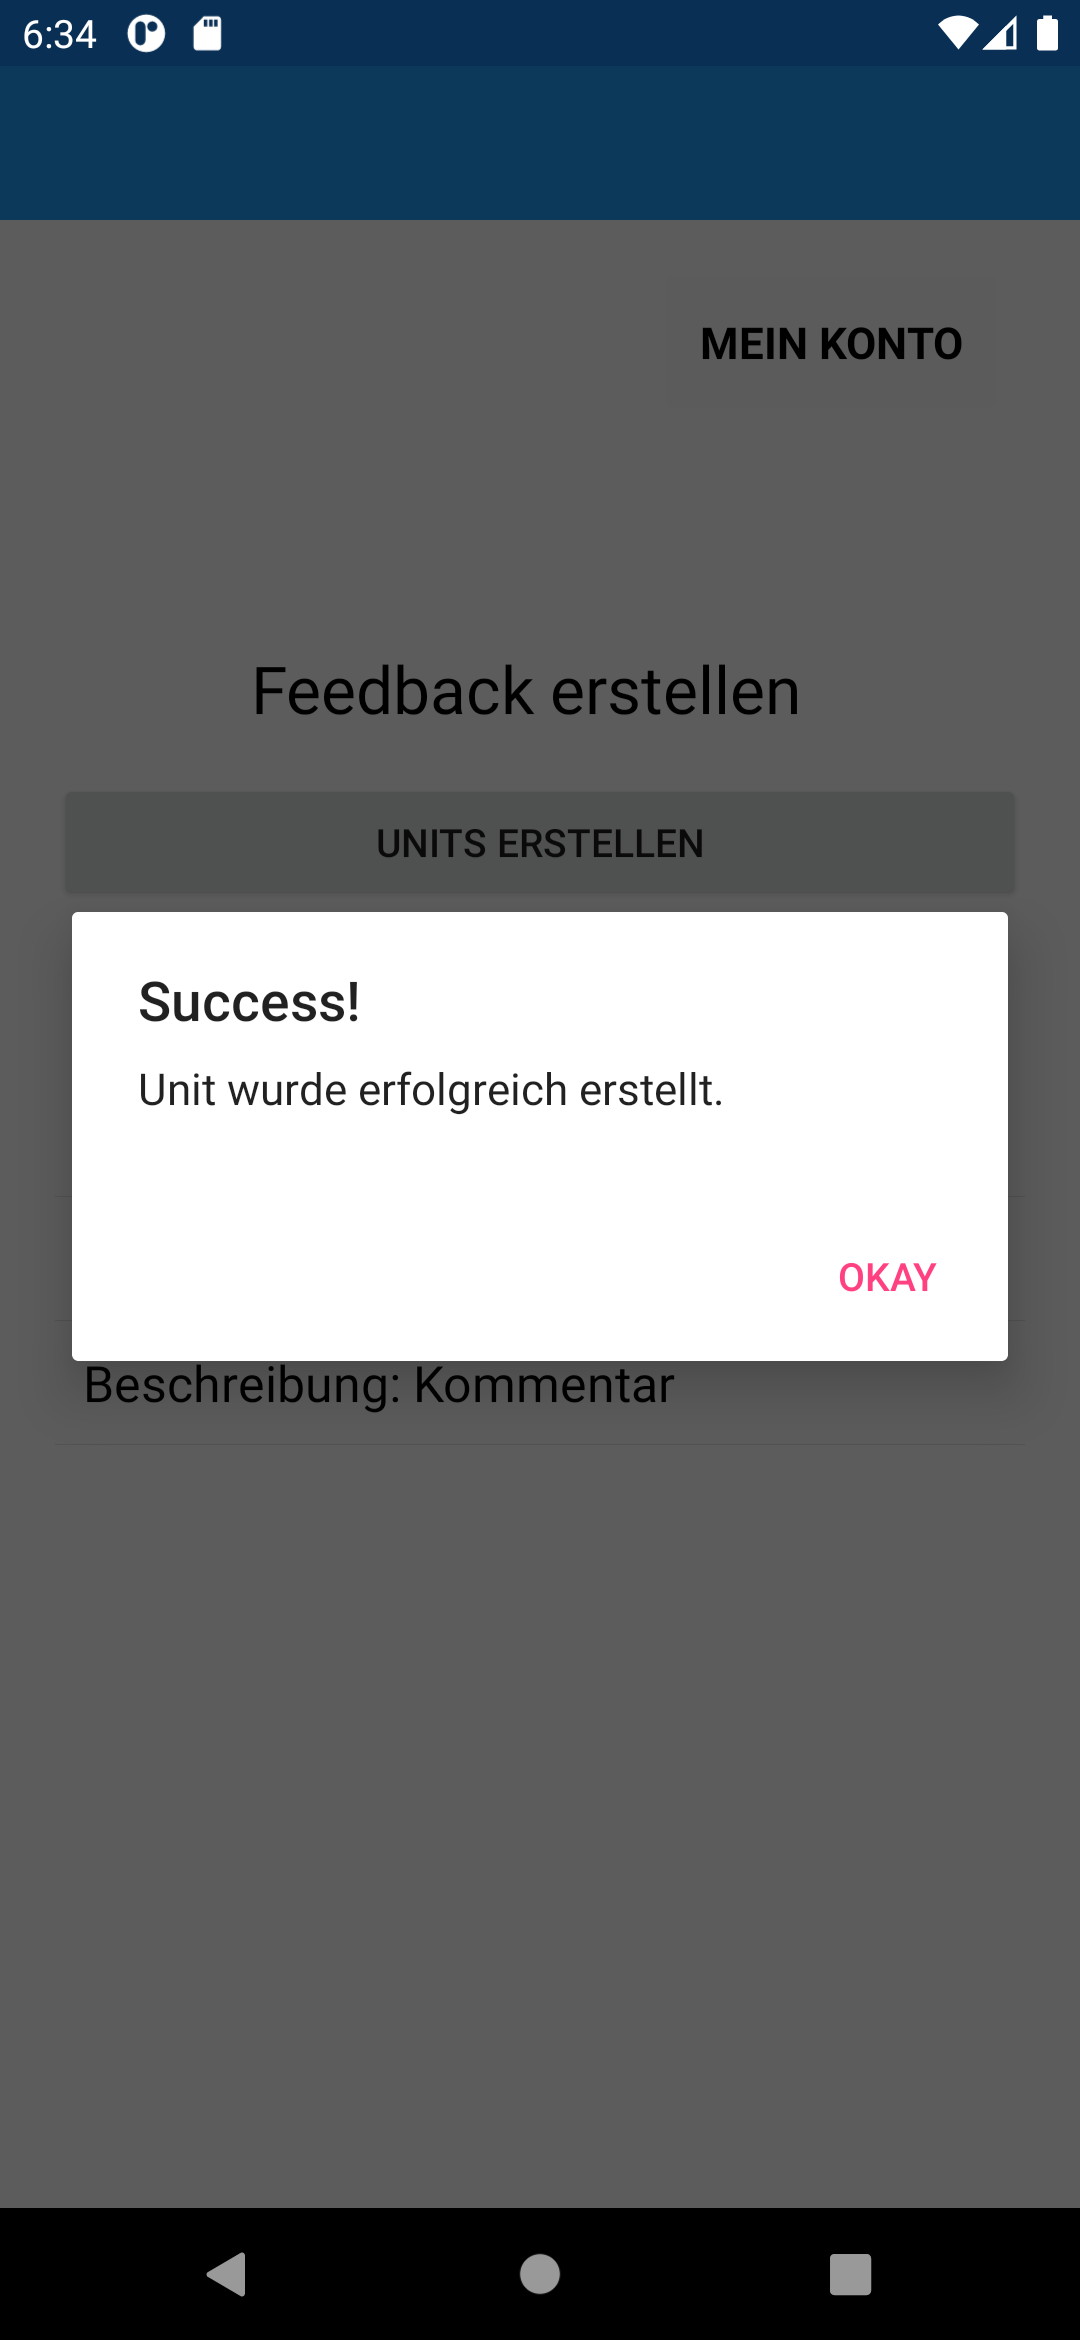
\includegraphics[width=4cm]{pics/Xamarin Lehrer/8.png}
        \caption[HomePage]{Unit erstellen}
    \end{center}
\end{figure}
\newpage

\section{Registrierung}
\begin{figure}[h]
    \begin{center}
        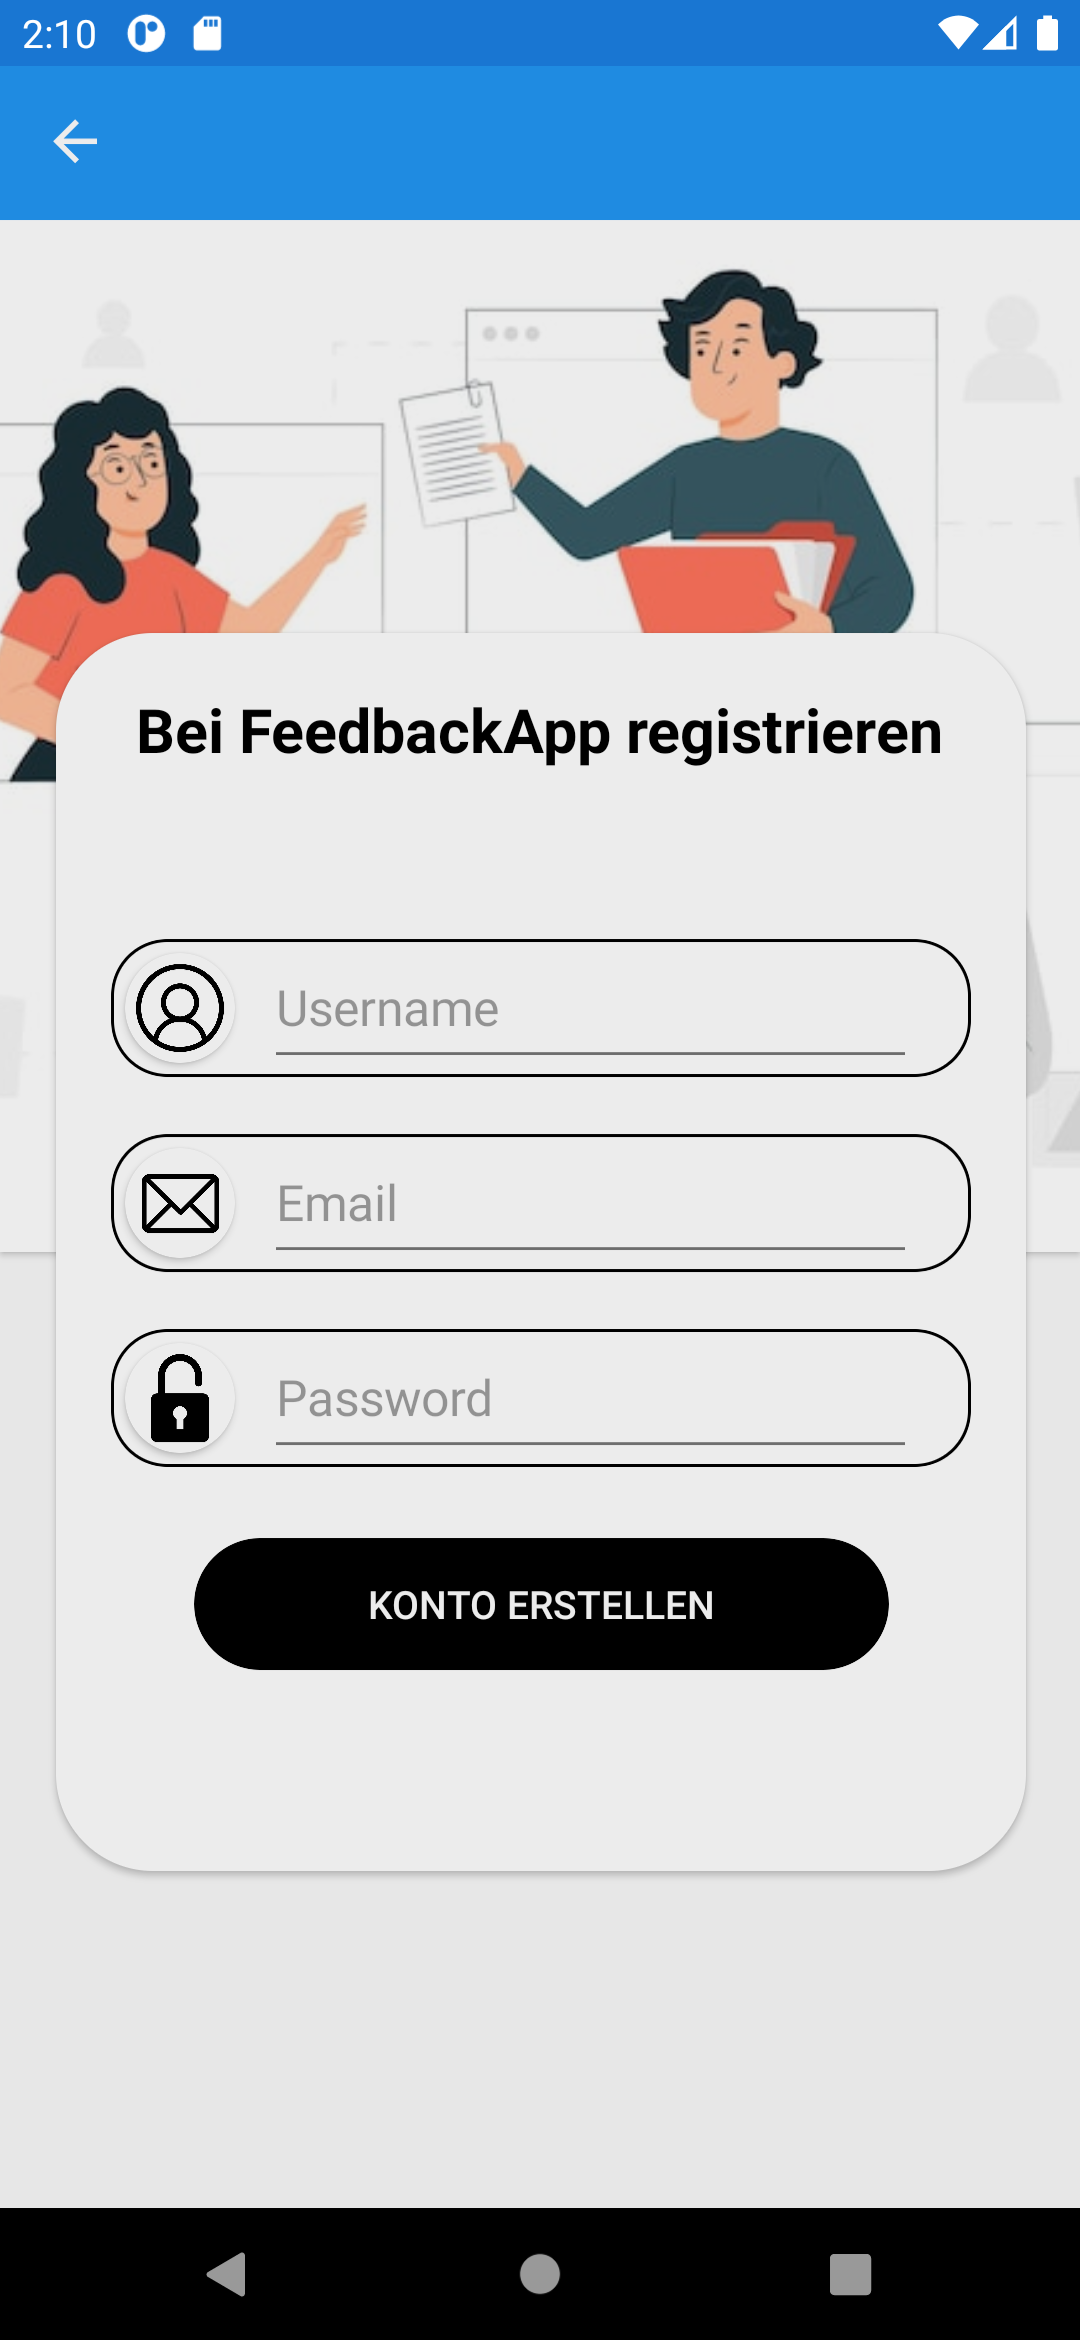
\includegraphics[width=5cm]{pics/Xamarin Student/2 Registration Page.png}
        \caption[Registrierung]{Registrierung Page Ansicht}
    \end{center}
\end{figure}
Die Registrierungsseite ist einfach und übersichtlich gestaltet. Um einen Benutzer zu registrieren, müssen Sie einen Benutzernamen, eine E-Mail-Adresse und ein Passwort eingeben. Nur Schüler können sich mit dieser Methode registrieren, während die Lehrerregistrierung so geschützt ist, dass Schüler sich nicht als Lehrer registrieren können und Lehrer ihr Profil vom Admin-Team erhalten.
\newpage
\begin{figure}[h]
    \begin{center}
        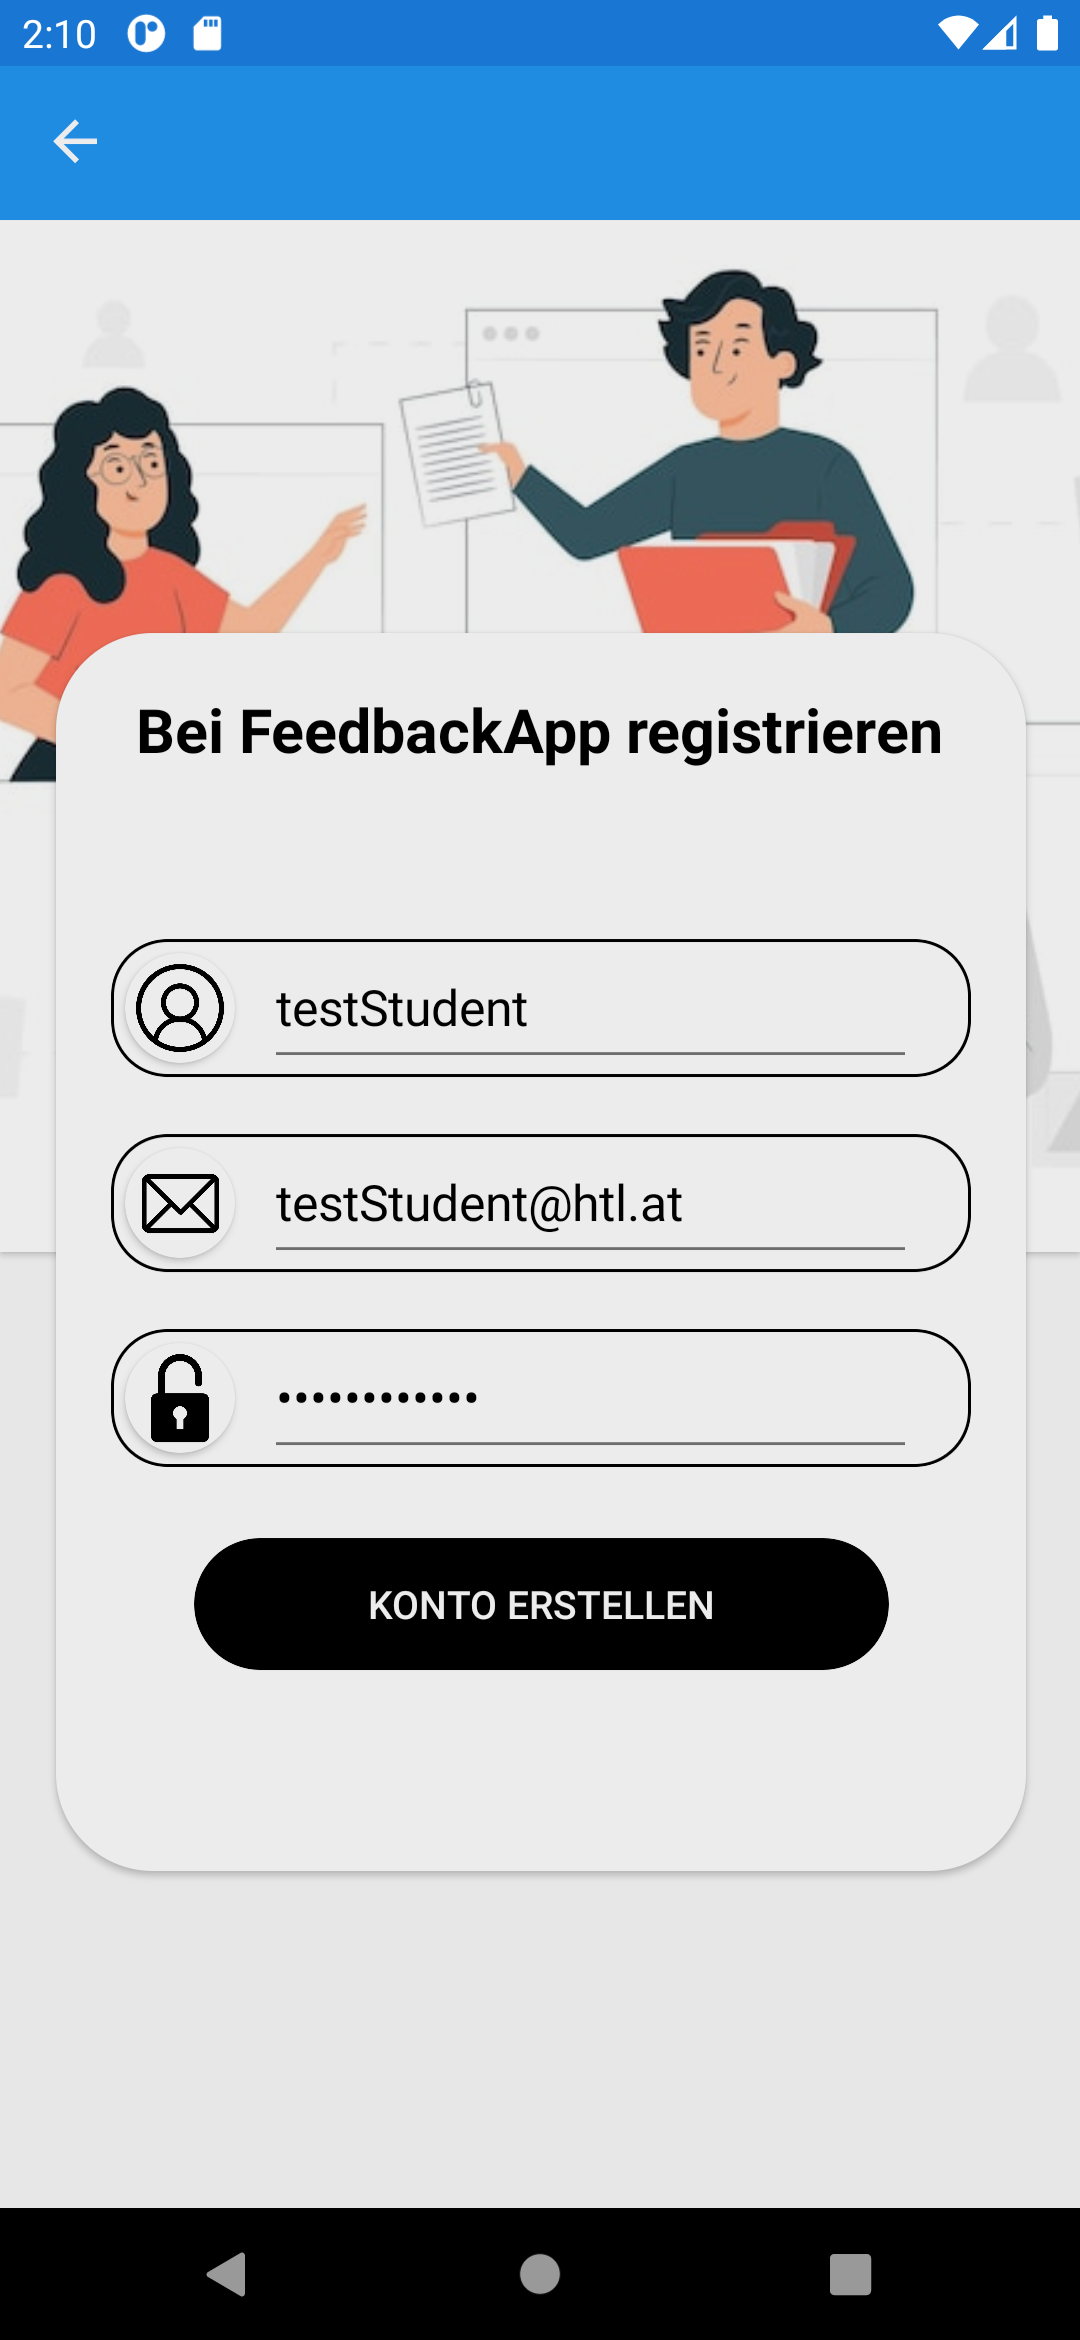
\includegraphics[width=4cm]{pics/Xamarin Student/3 Registration Page Full.png}\hfill
        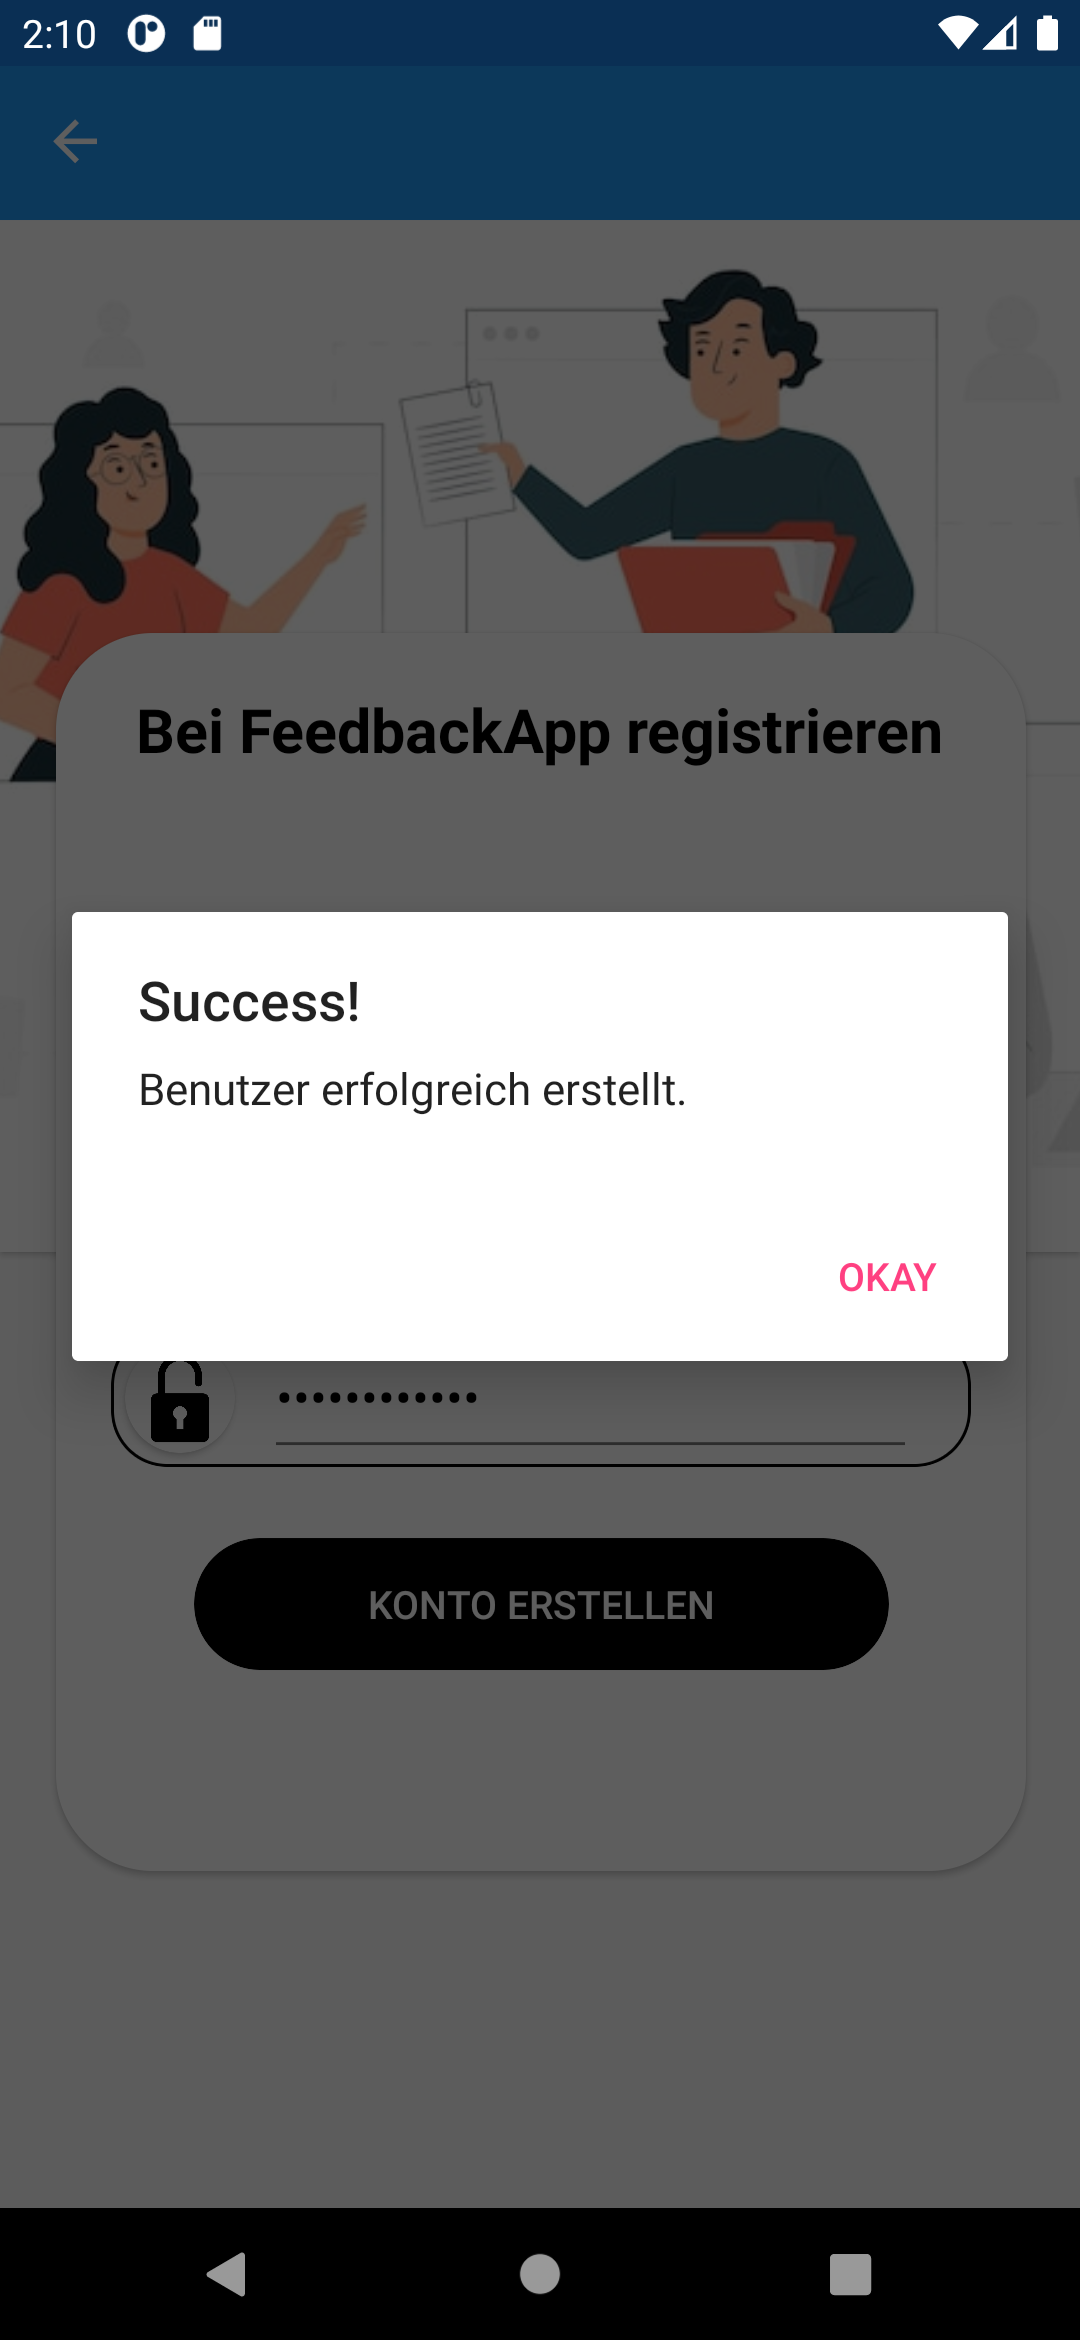
\includegraphics[width=4cm]{pics/Xamarin Student/4 Registration Page Success.png}
        \caption[Registrierung]{Benutzerkonto erstellen}
    \end{center}
\end{figure}
Falls die Daten falsch sind, d.h. die nicht den Regeln des Codes unterliegen, erhalten wir per E-Mail eine Warnung und einen Fehler, um die Registrierungsaktion zu wiederholen.
\newpage

\section{Benutzerkontoverwaltung}
Im Profil kann der Benutzer seine gespeicherten Daten wie Passwort, Vorname oder
Schule aktualisieren.
\begin{figure}[h]
    \begin{center}
        \includegraphics*[width=5cm]{pics/Xamarin Student/13 My Acc.png}
        \caption[MyAccount]{Benutzerkontoverwaltung Student Ansicht}
    \end{center}
\end{figure}
\newpage
Sobald wir die Benutzerkontoseite betreten, sehen wir, dass der Name, der Nachname und der Name der Schule, die wir besuchen, fehlt. Mit den Buttons auf der rechten Seite können wir jeden einzeln eingeben, ändern oder löschen. Auch die E-Mail ist bereits gespeichert, die wir bei der Registrierung eingegeben haben, die aber später geändert werden kann.
\begin{figure}[h]
    \begin{center}
    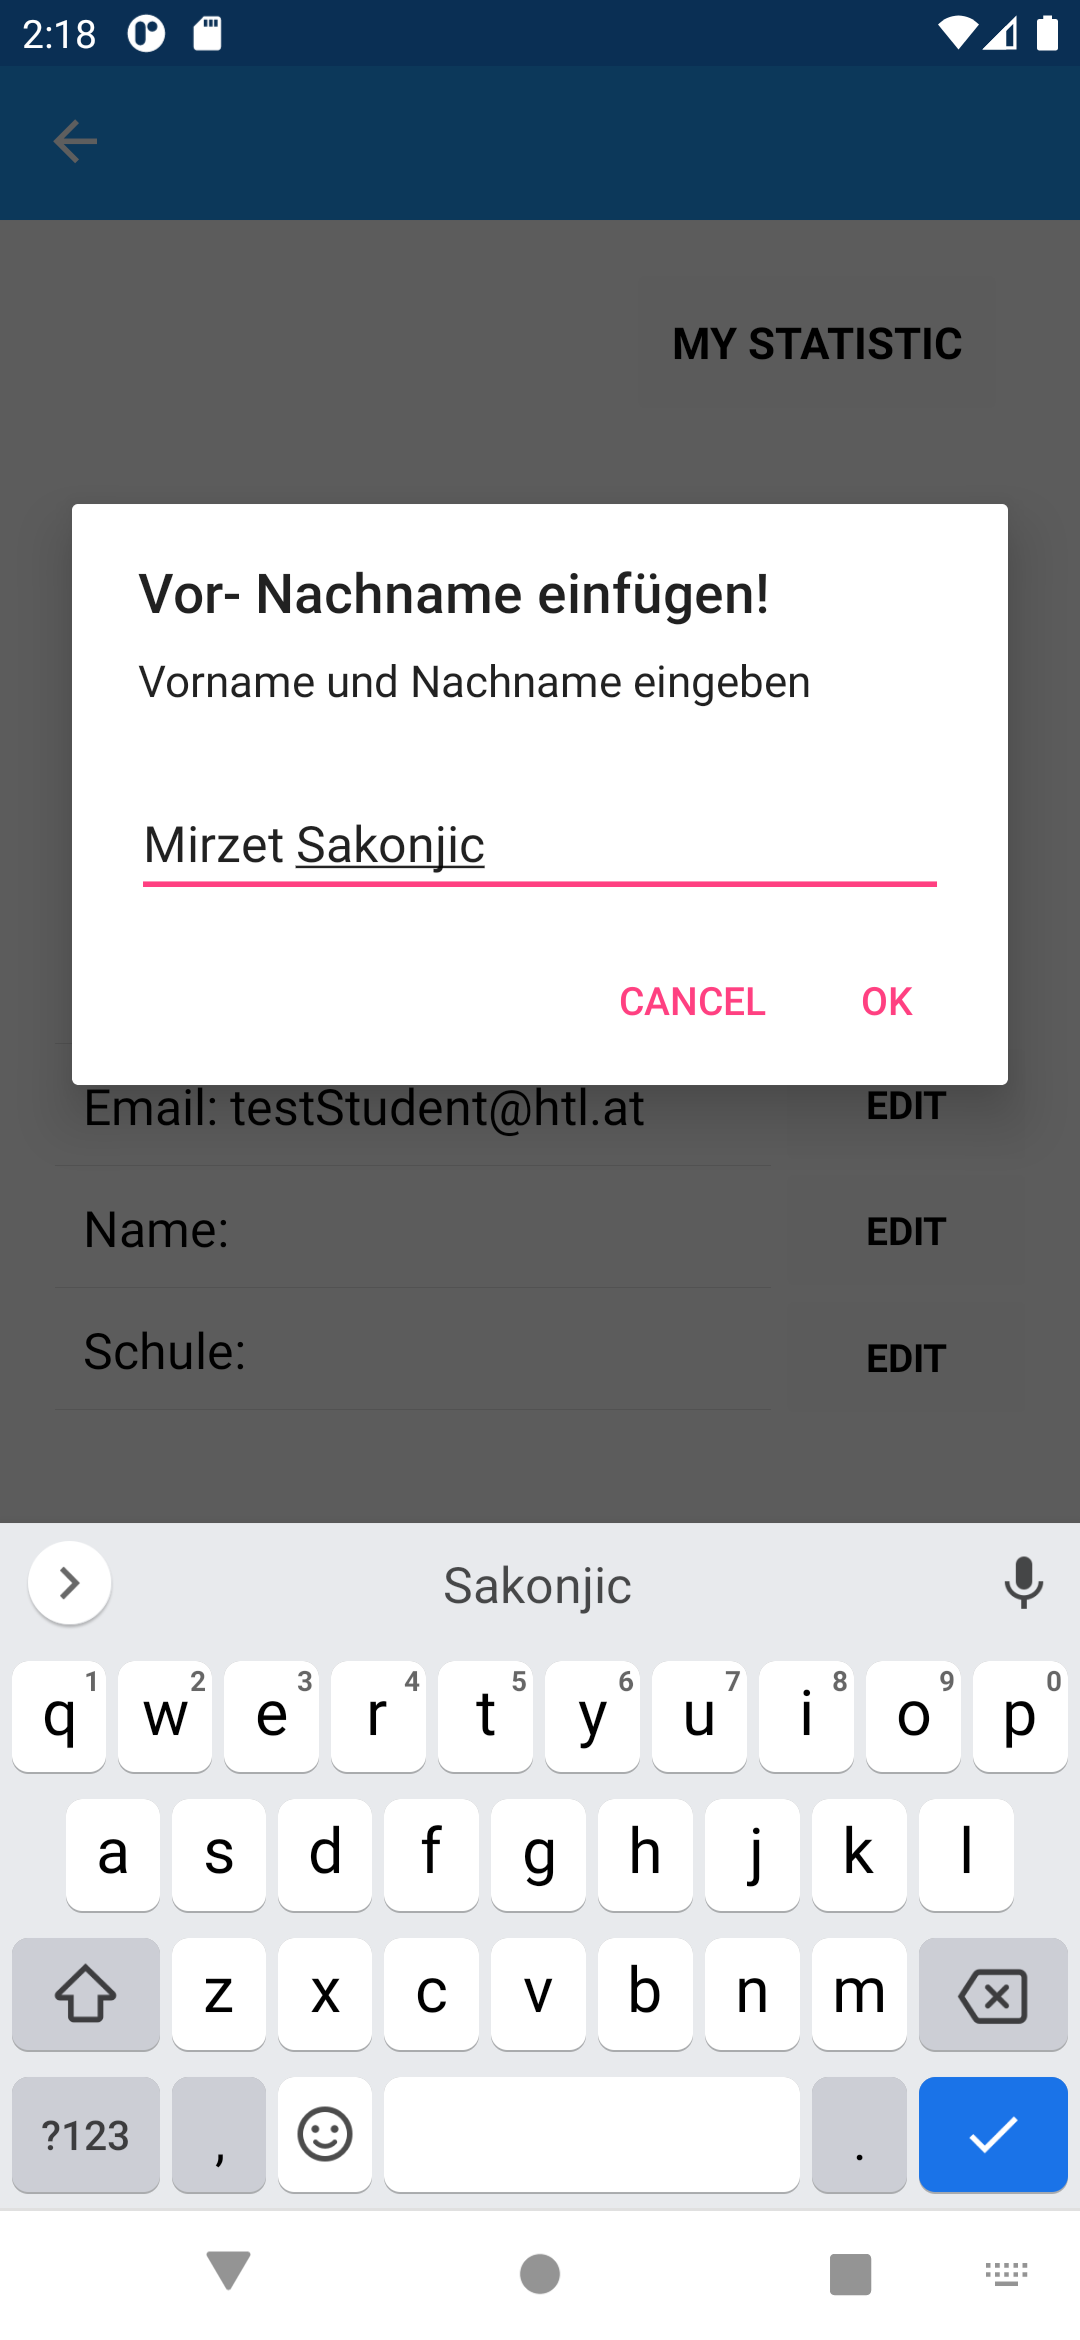
\includegraphics[width=4cm]{pics/Xamarin Student/14 Name.png}\hfill
    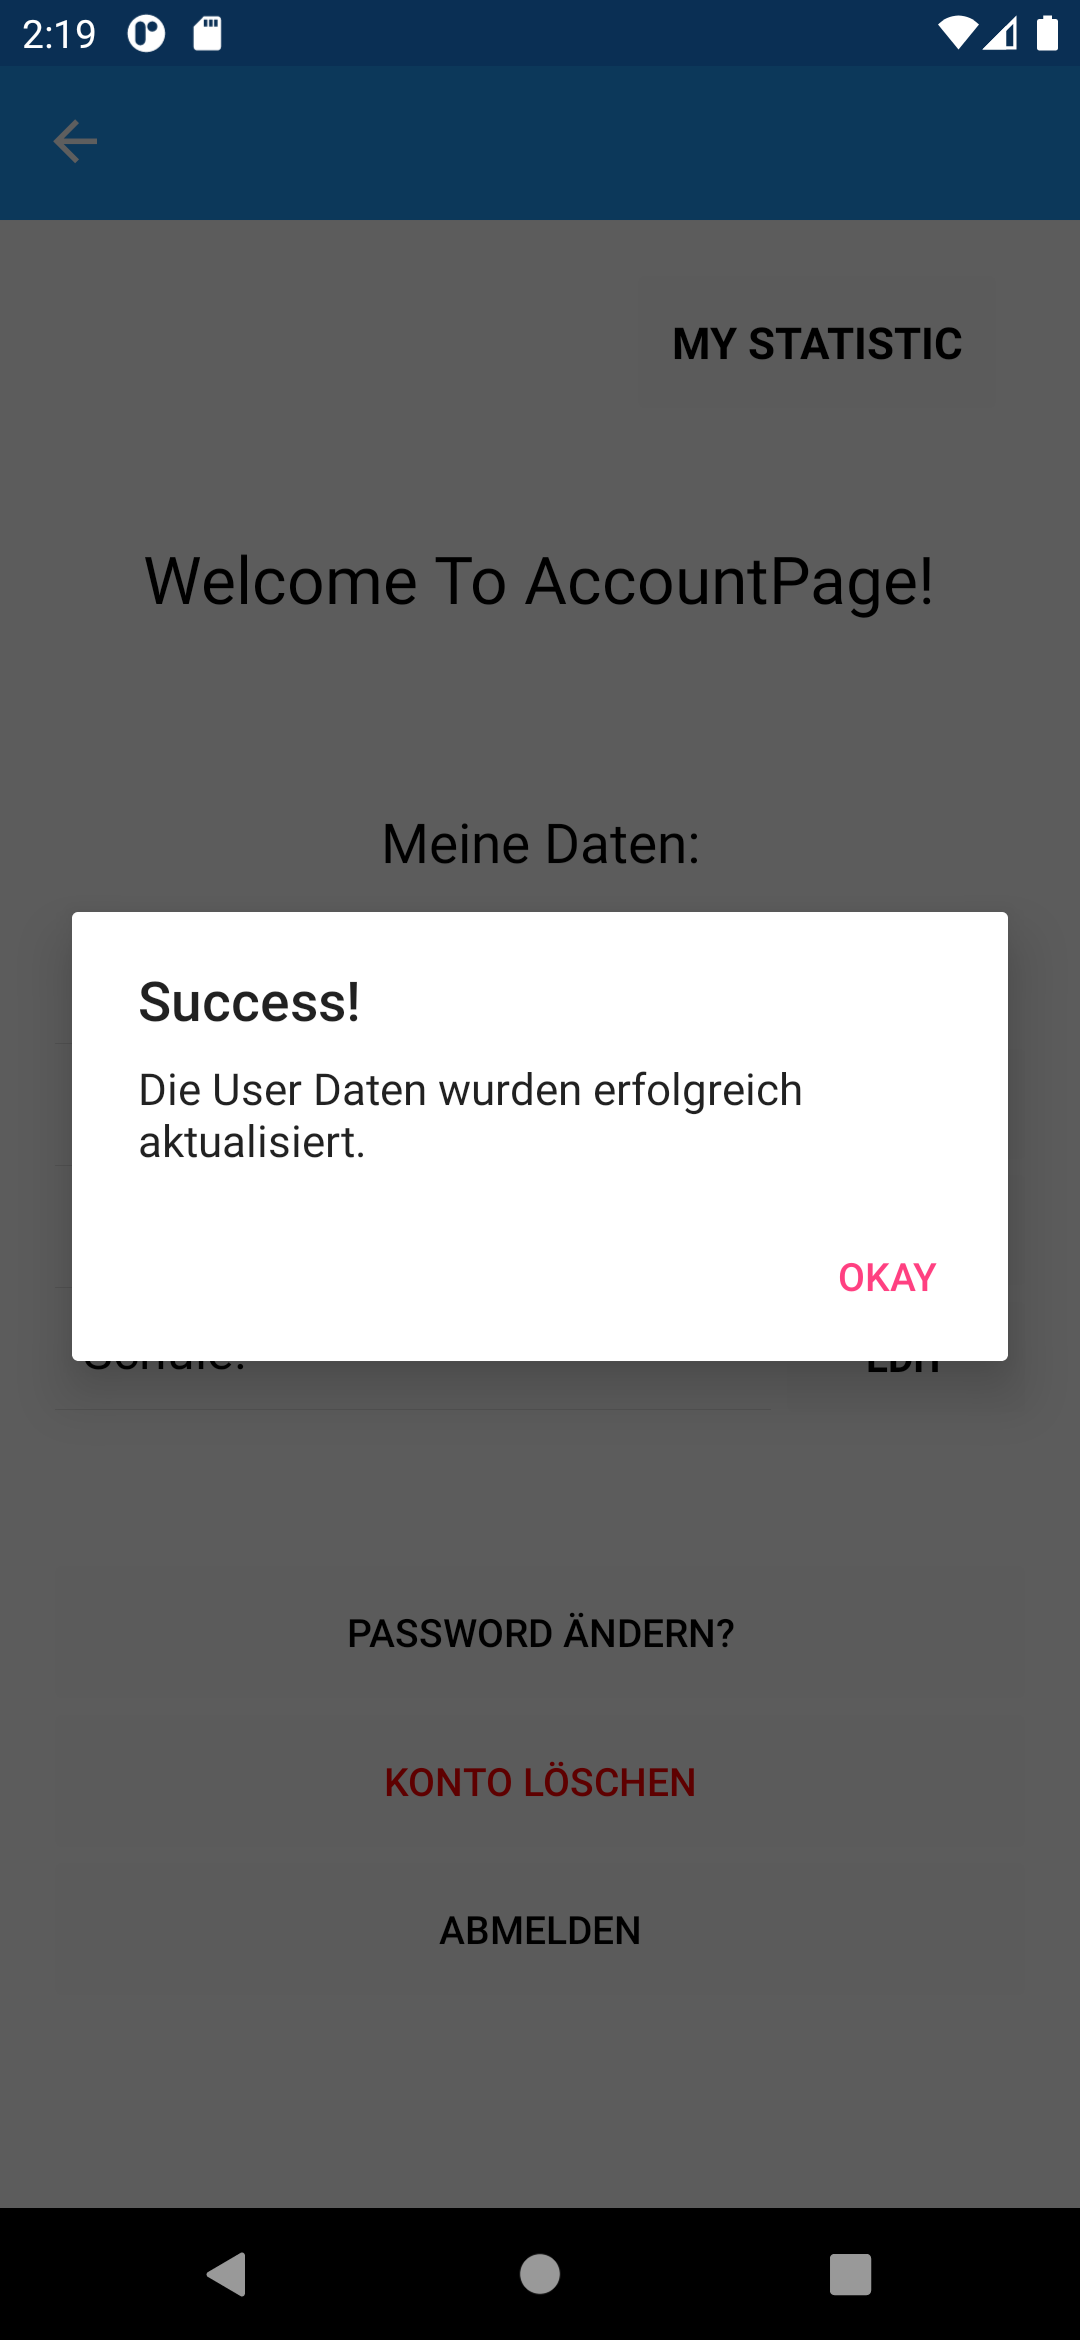
\includegraphics[width=4cm]{pics/Xamarin Student/15 Name success.png}\hfill
    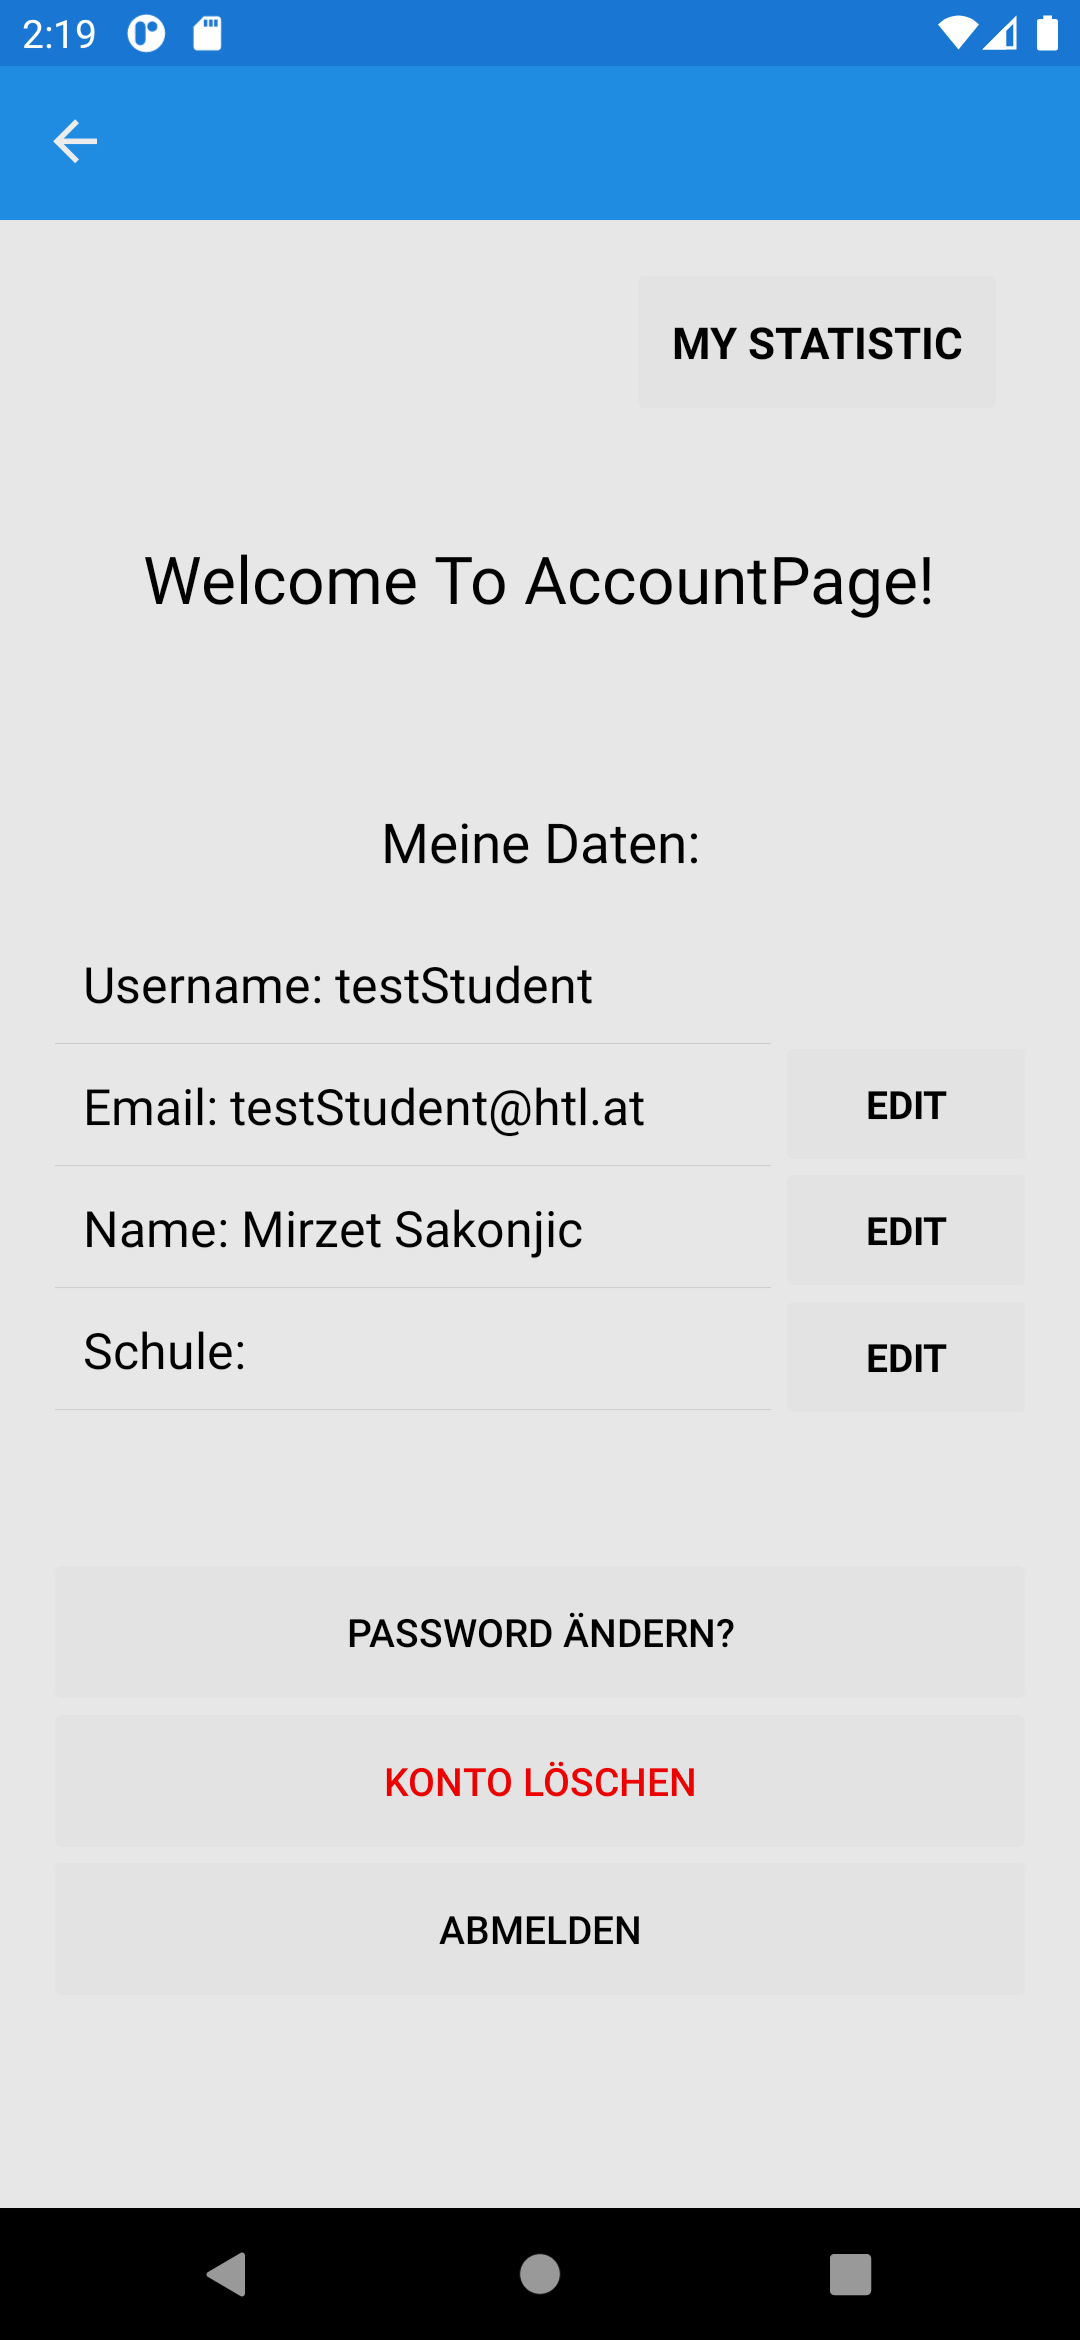
\includegraphics[width=4cm]{pics/Xamarin Student/16 Name.png}
    \caption[MyAccount]{Namensänderung}
    \end{center}
\end{figure}
\newpage
Als nächstes geben Sie den Namen der Schule ein, die wir besuchen, oder des Hauptfachs, das wir studieren.
\begin{figure}[h]
    \begin{center}
    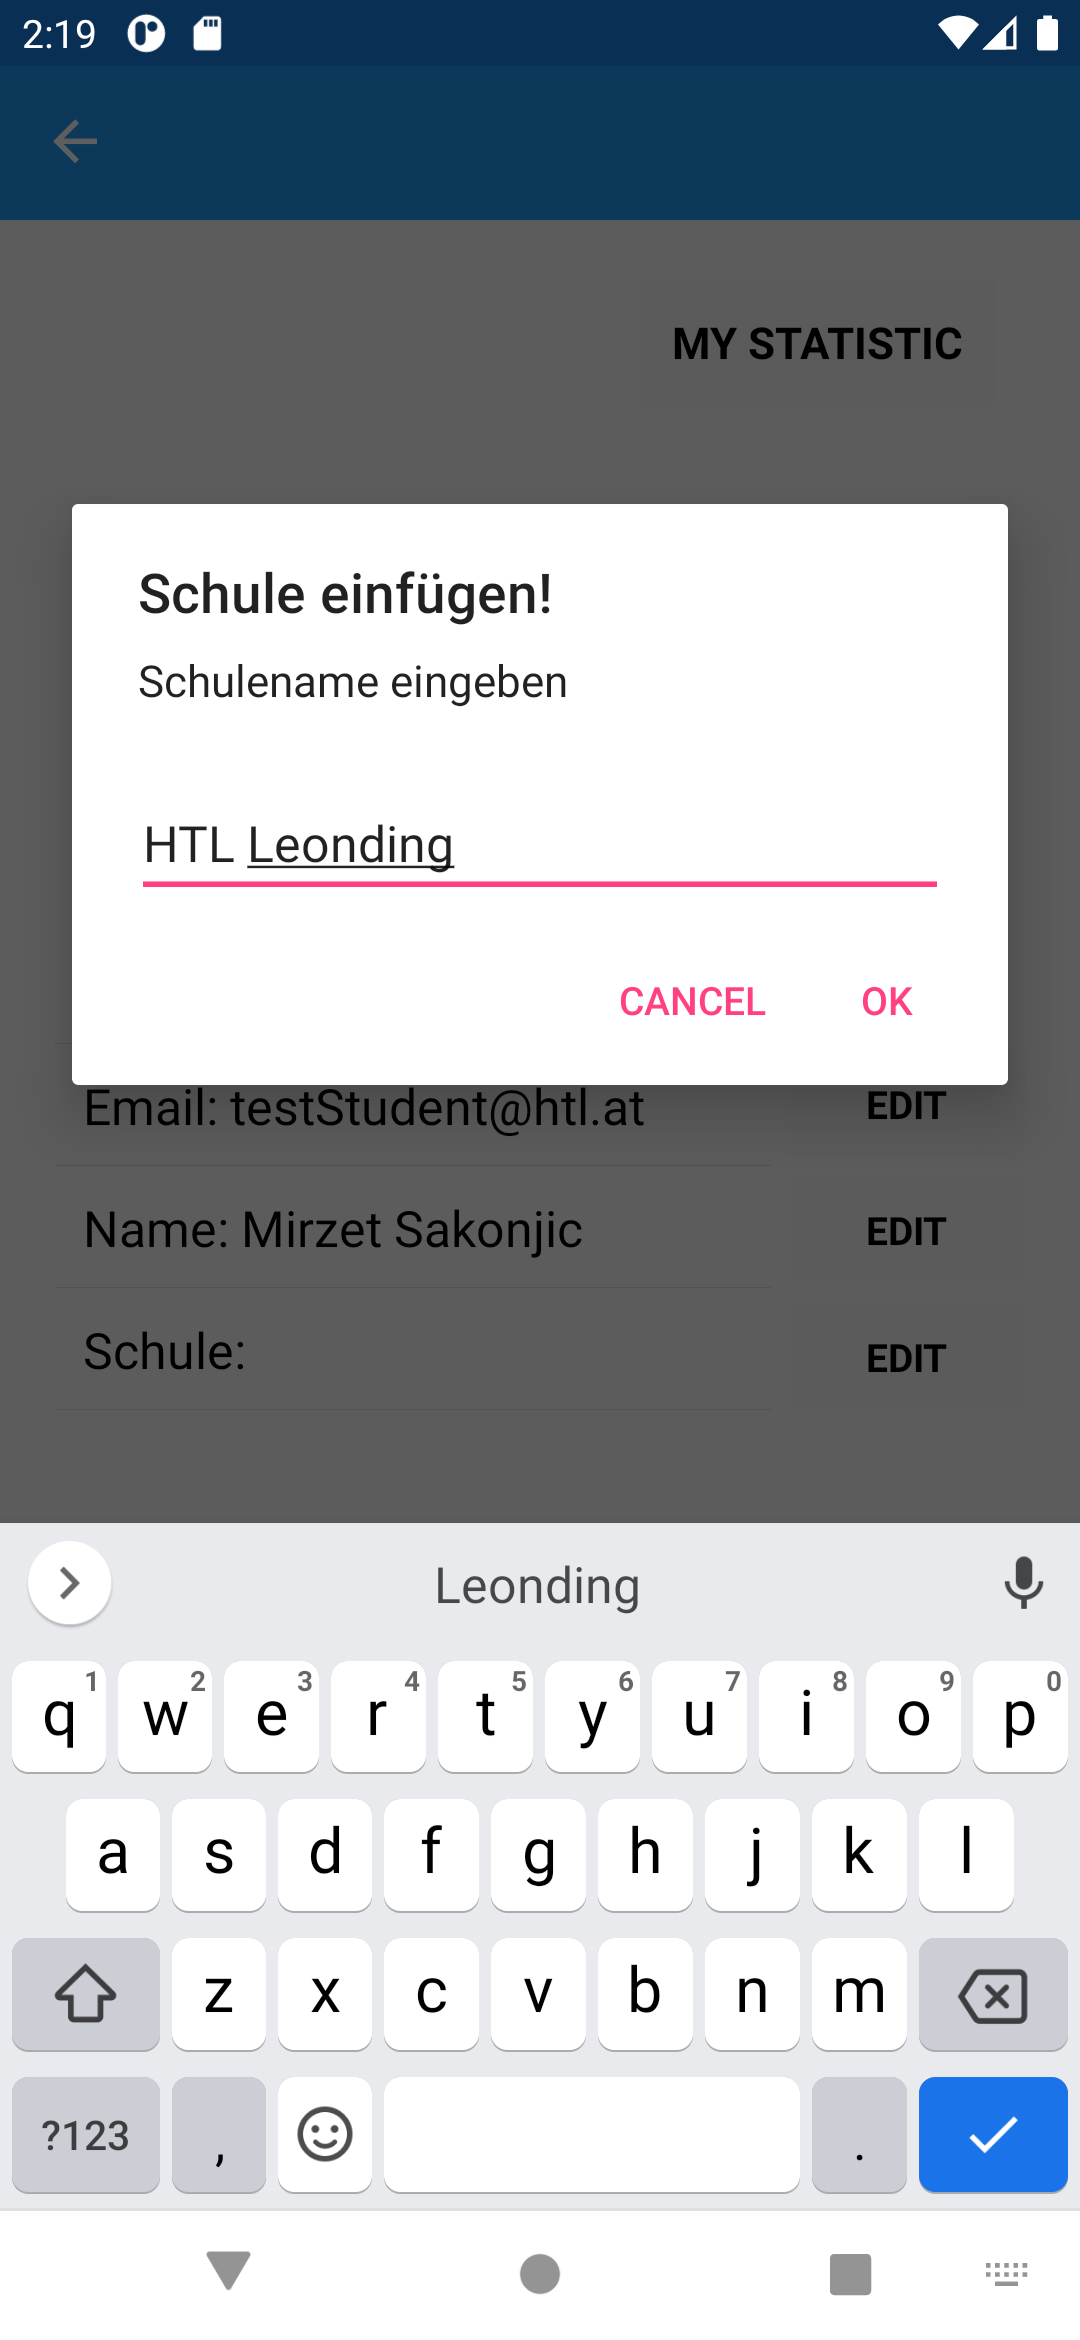
\includegraphics[width=4cm]{pics/Xamarin Student/17 School.png}\hfill
    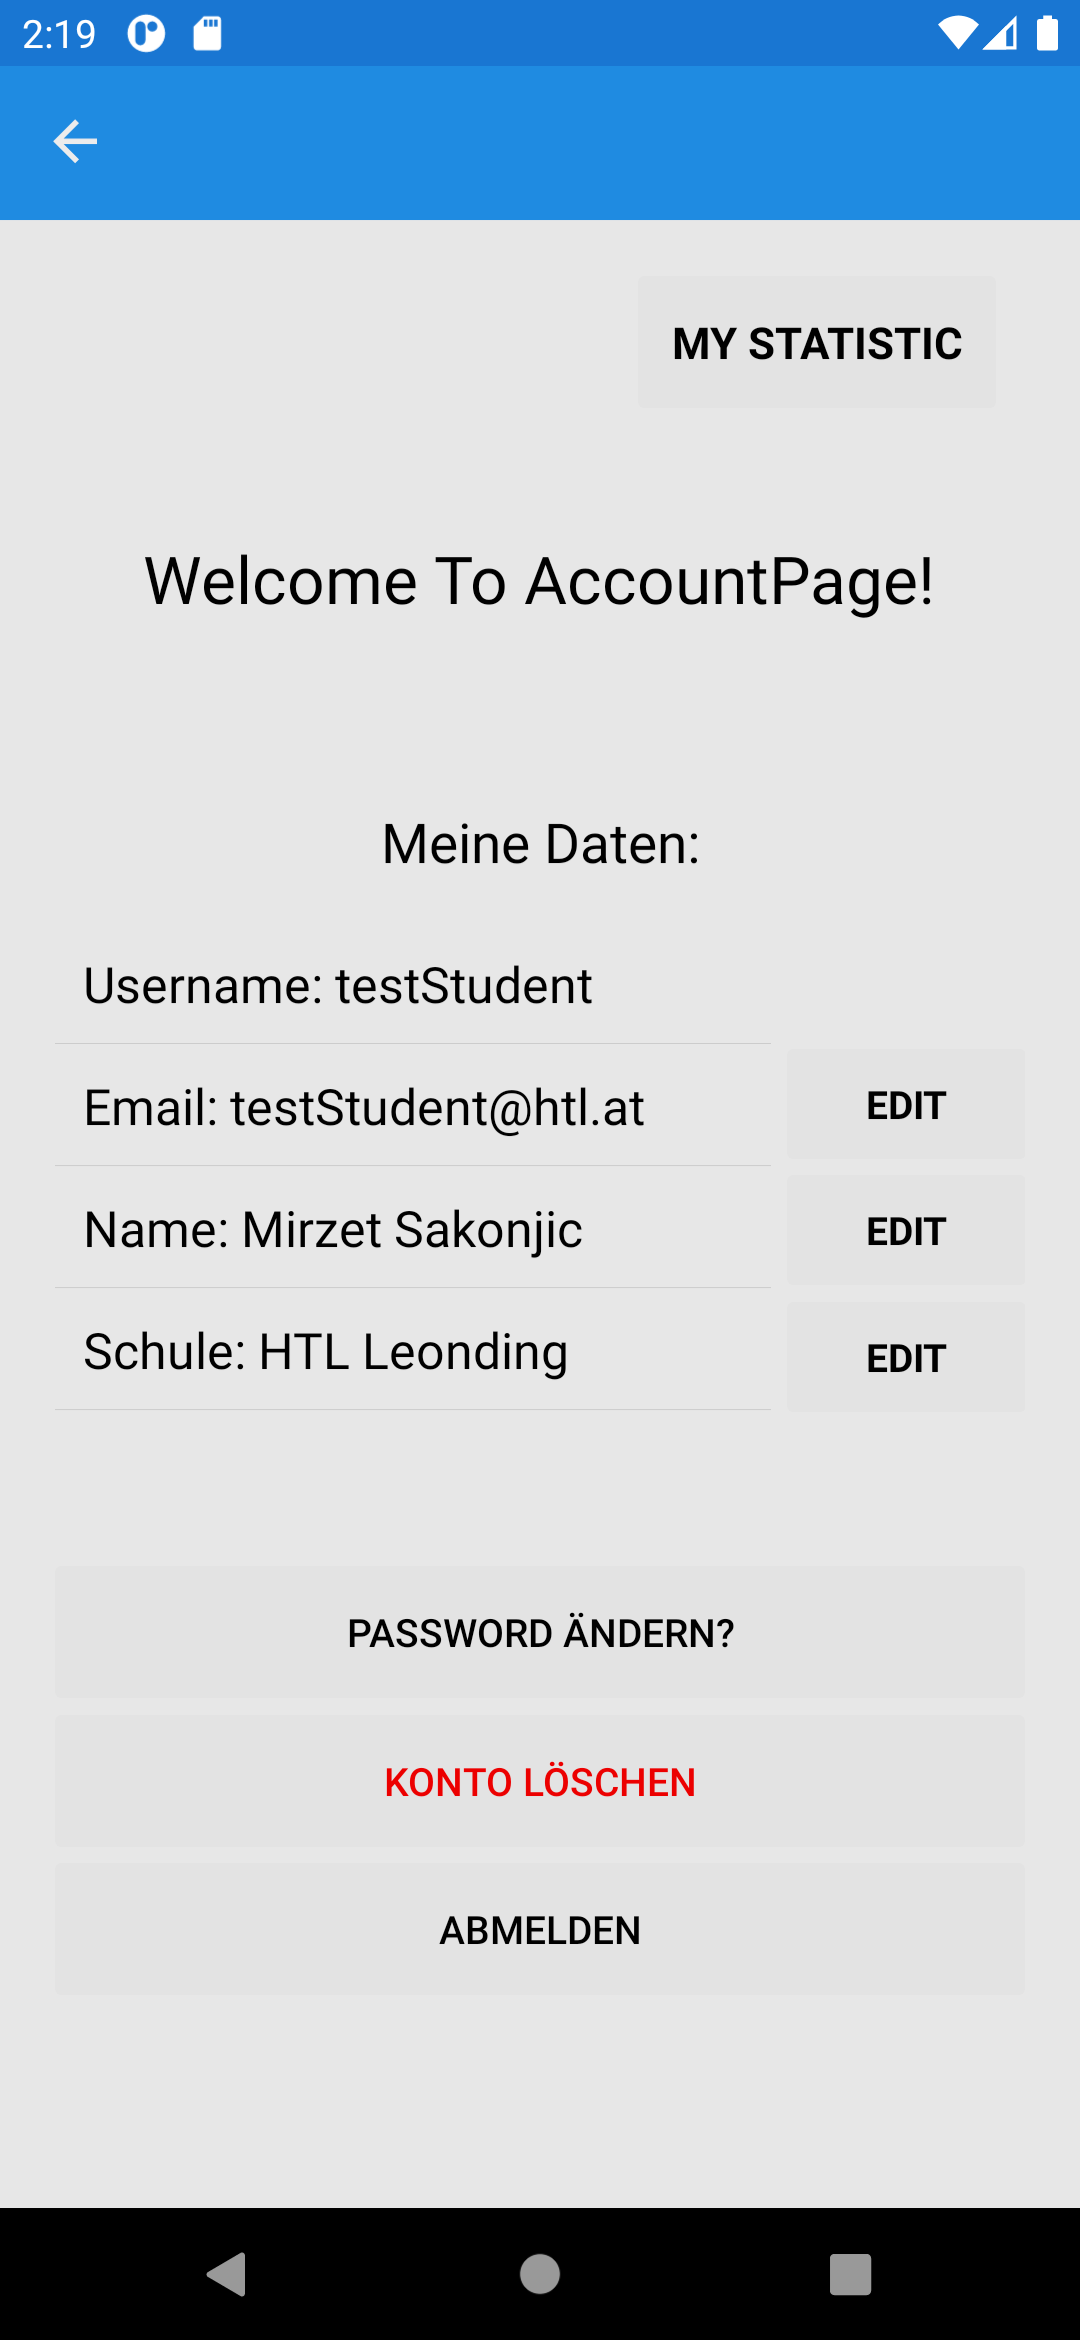
\includegraphics[width=4cm]{pics/Xamarin Student/18 School success.png}
    \caption[MyAccount]{Umbenennung der Schule}
    \end{center}
\end{figure}
\newpage
Falls wir die E-Mail-Adresse ändern und eine neue eingeben möchten, ist dies ebenfalls möglich. Falls die neue E-Mail-Adresse falsch ist oder die Kriterien für die E-Mail-Adresse nicht erfüllt, erhalten wir eine Fehlermeldung.
\begin{figure}[h]
    \begin{center}
    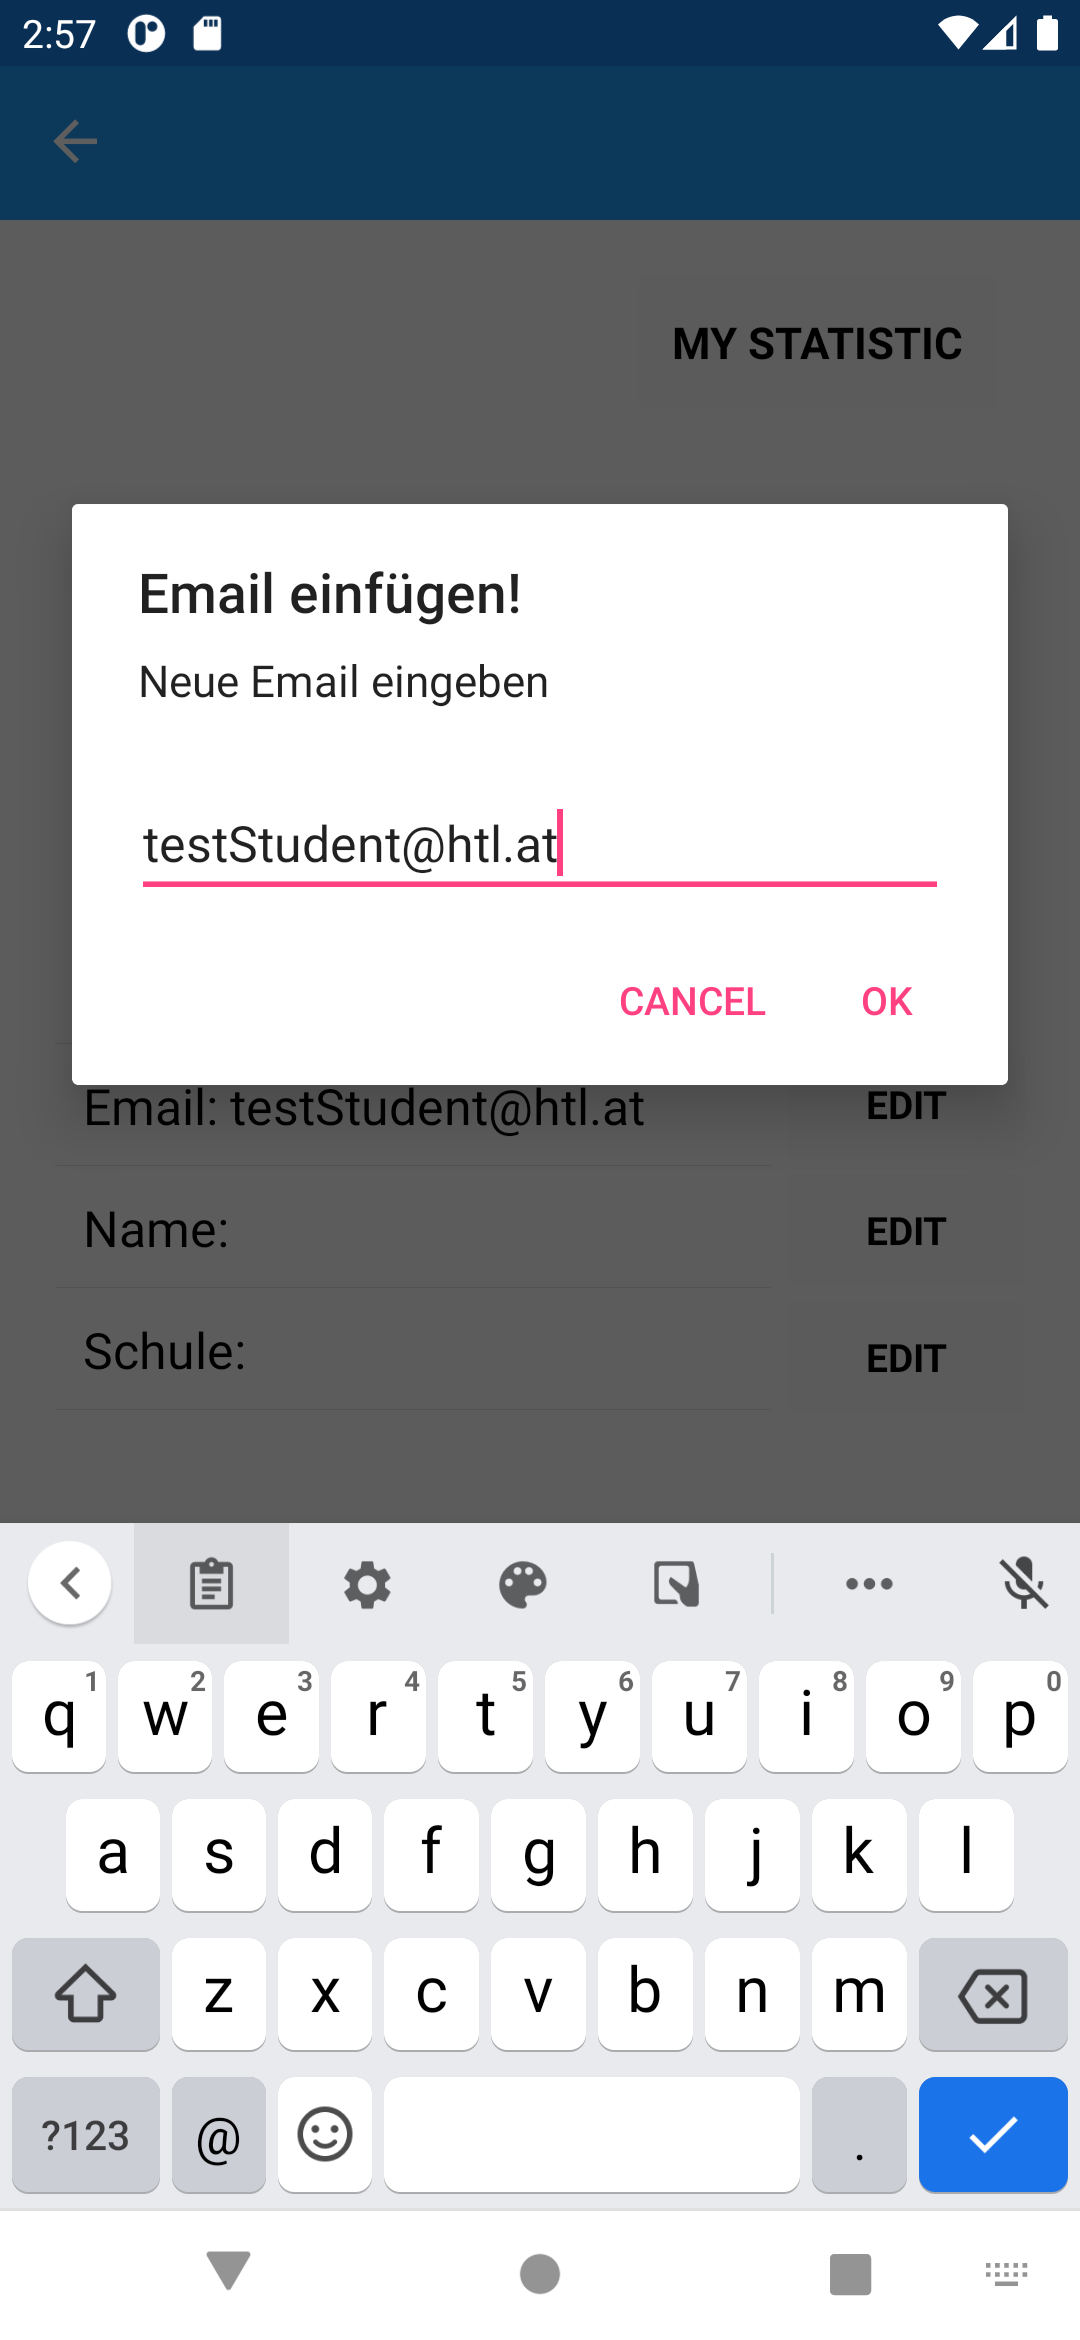
\includegraphics[width=4cm]{pics/Xamarin Student/26 New Email.png}\
    \caption[MyAccount]{Änderung der E-Mail-Adresse}
    \end{center}
\end{figure}
\newpage
Wir werden das Passwort ändern, indem wir zuerst das alte Passwort und dann das neue eingeben. Wenn das alte Passwort korrekt ist und somit das neue Passwort den Passwortkriterien unterliegt, wird das neue Passwort gespeichert.
\begin{figure}[h]
    \begin{center}
    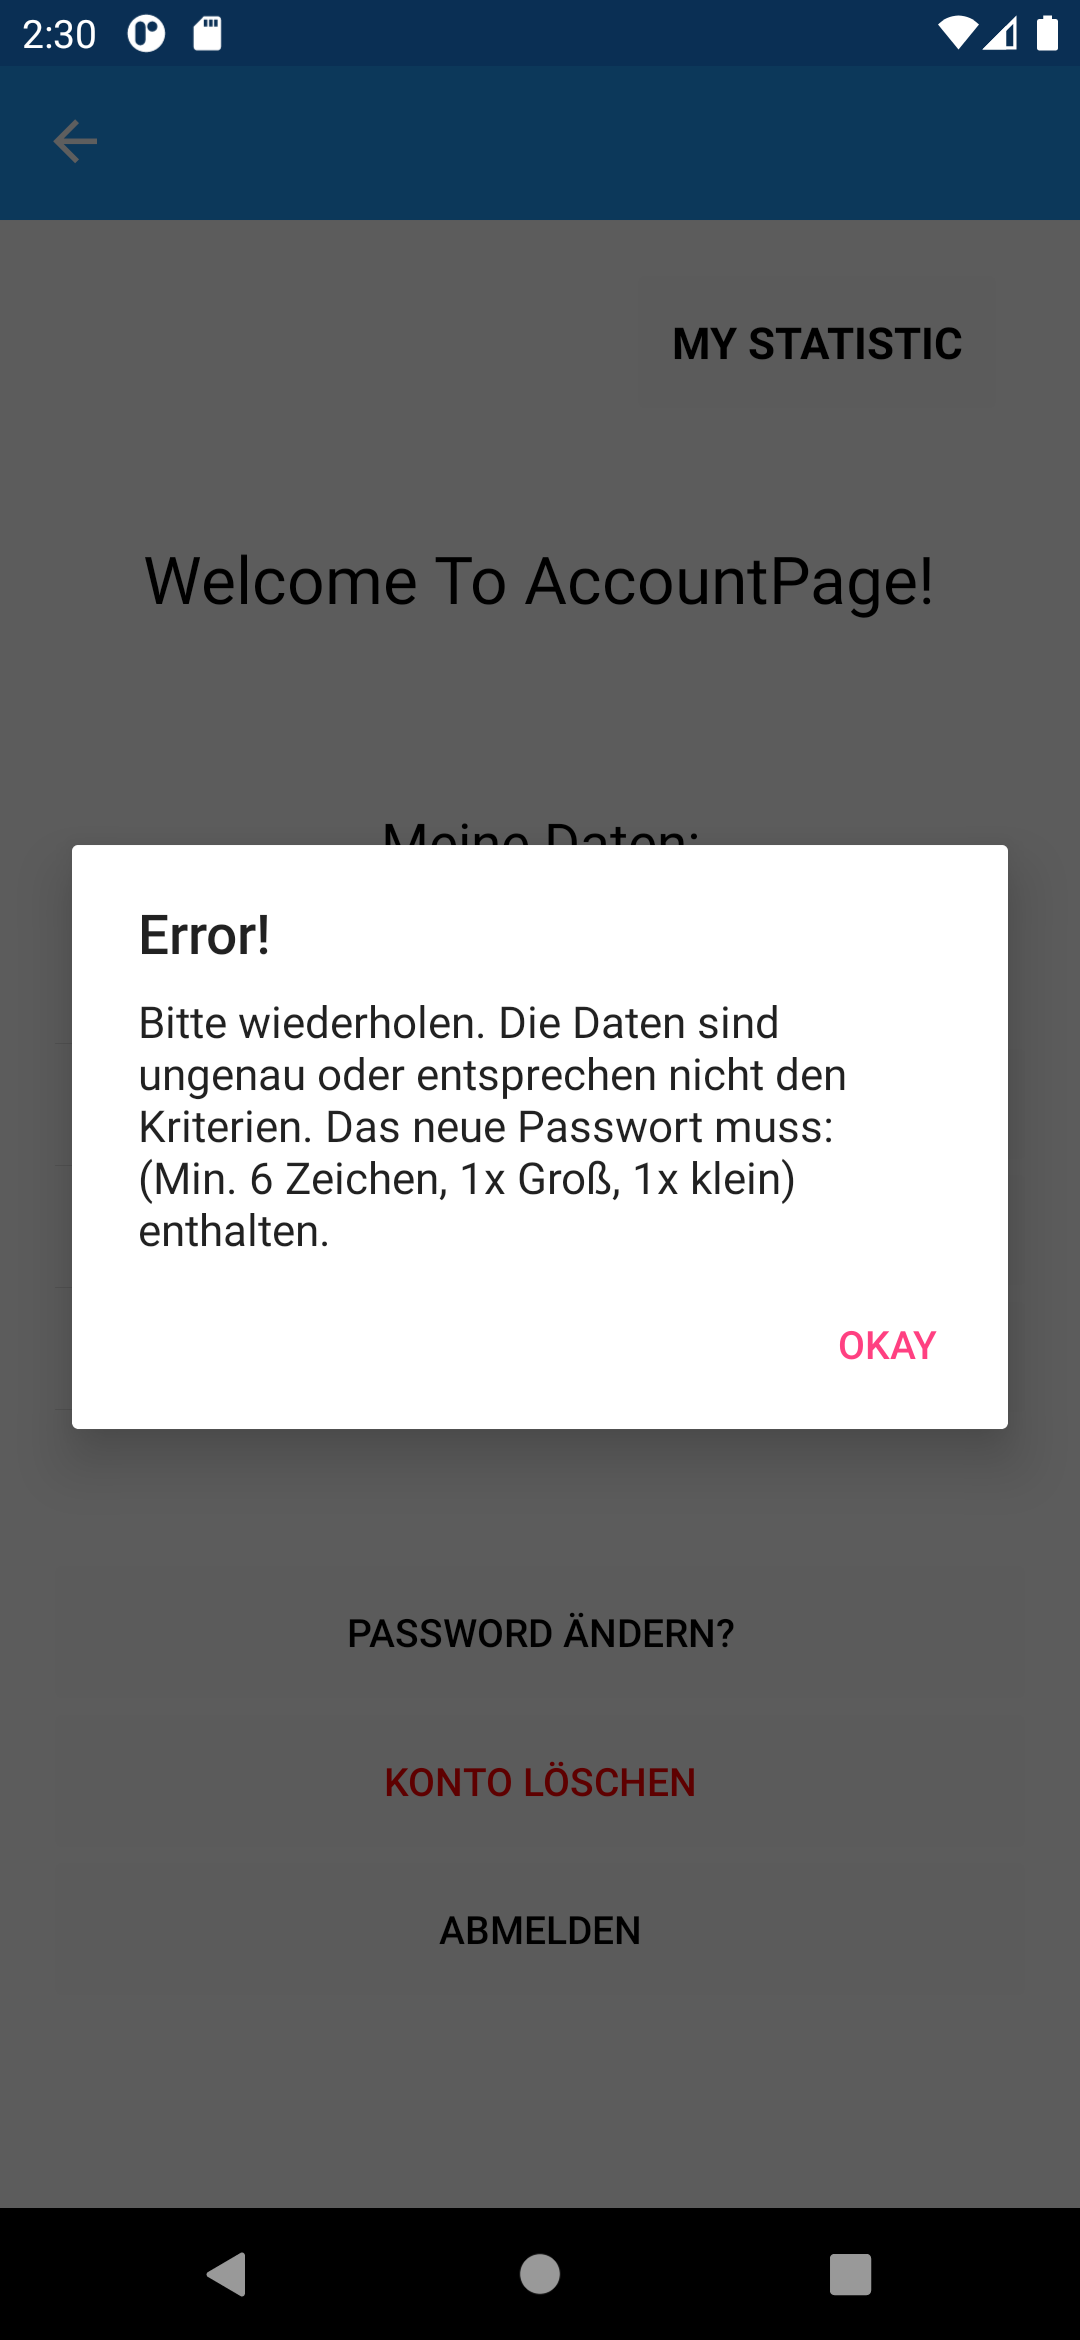
\includegraphics[width=3cm]{pics/Xamarin Student/19 Pass change.png}\hfill
    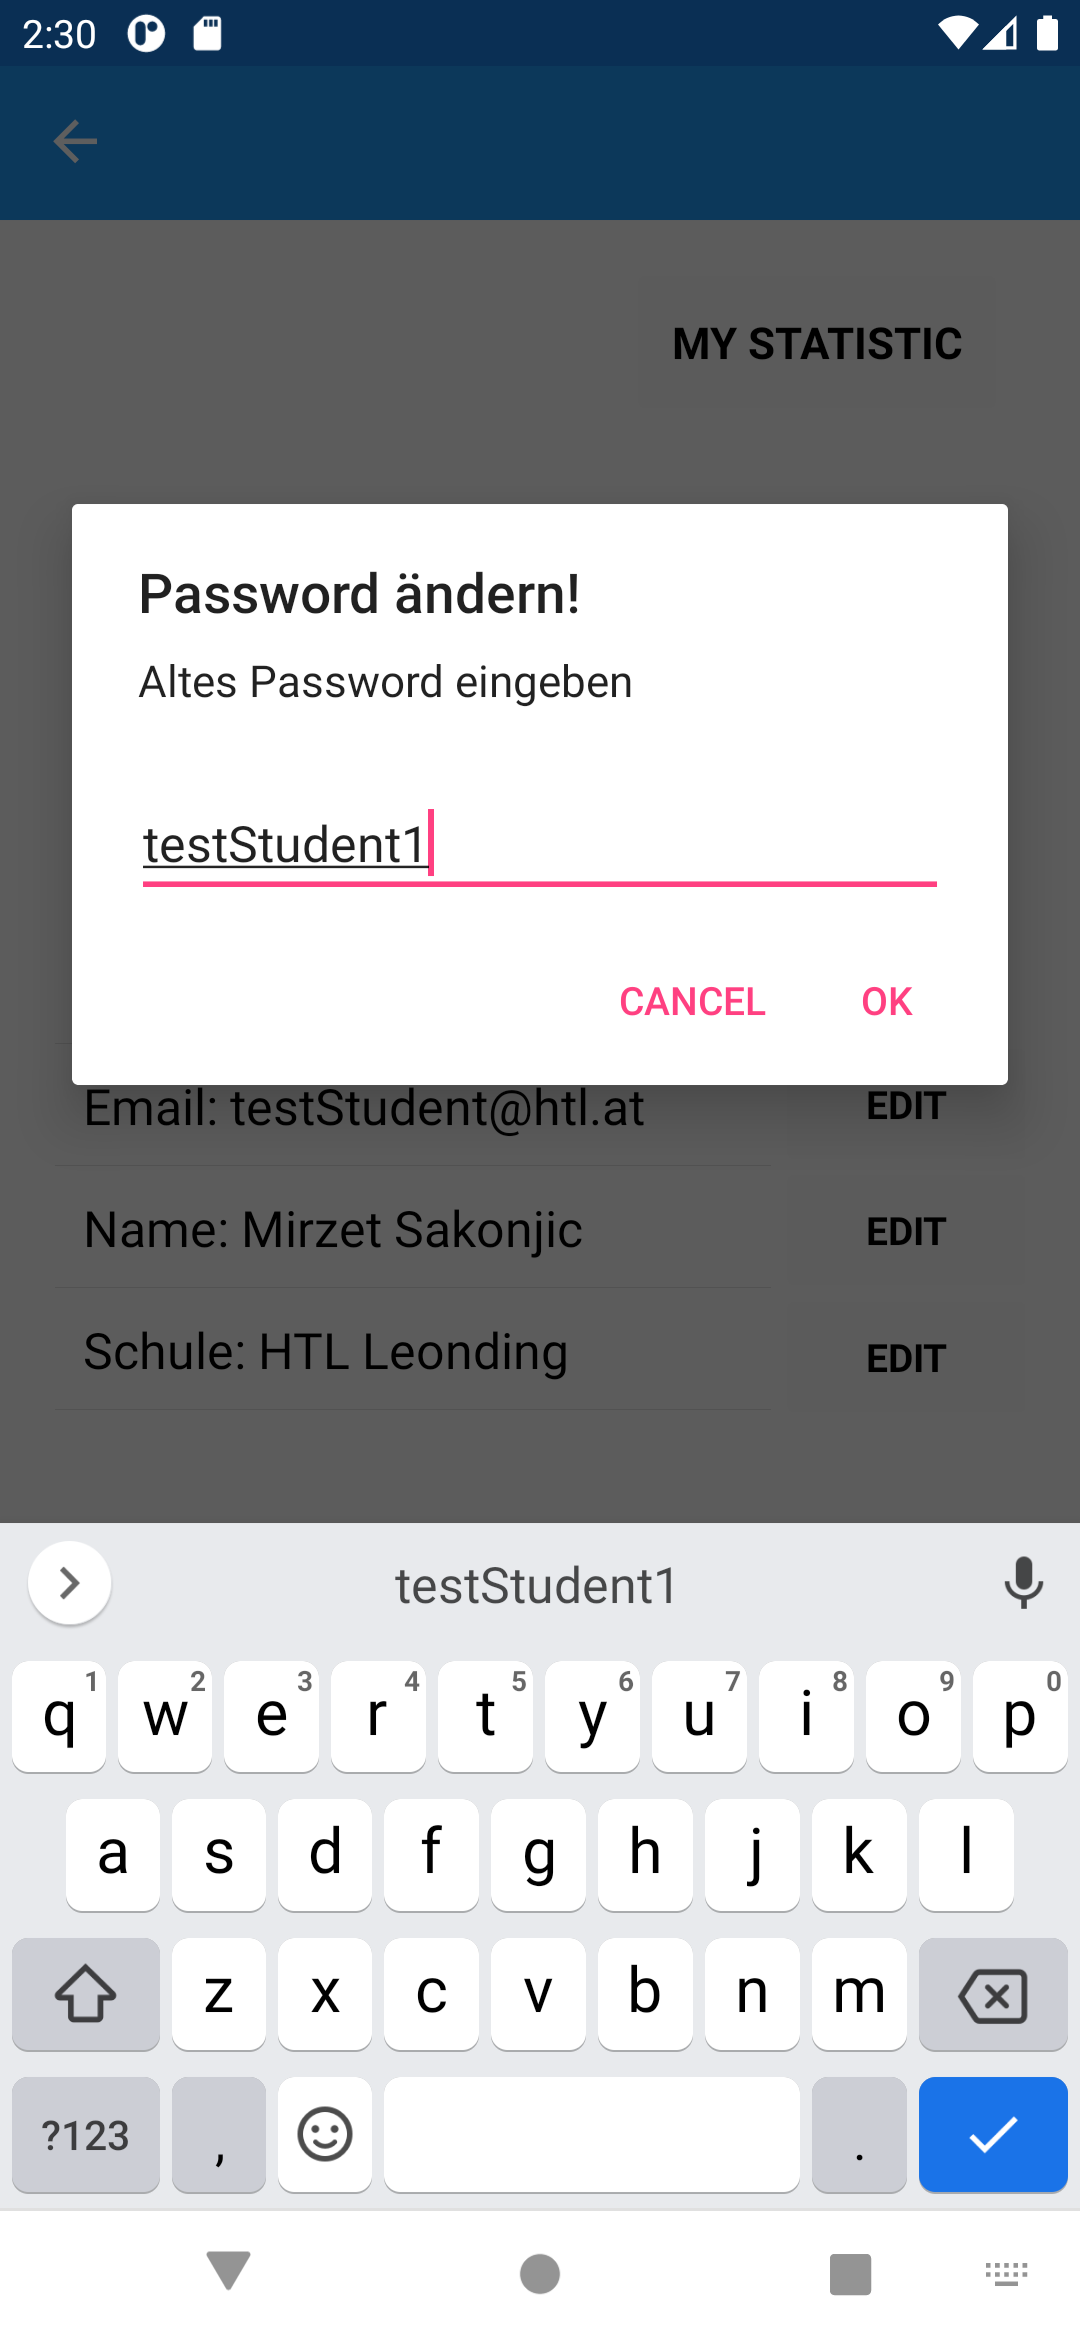
\includegraphics[width=3cm]{pics/Xamarin Student/20.png}
    \end{center}
\end{figure}
\begin{figure}[h]
    \begin{center}
    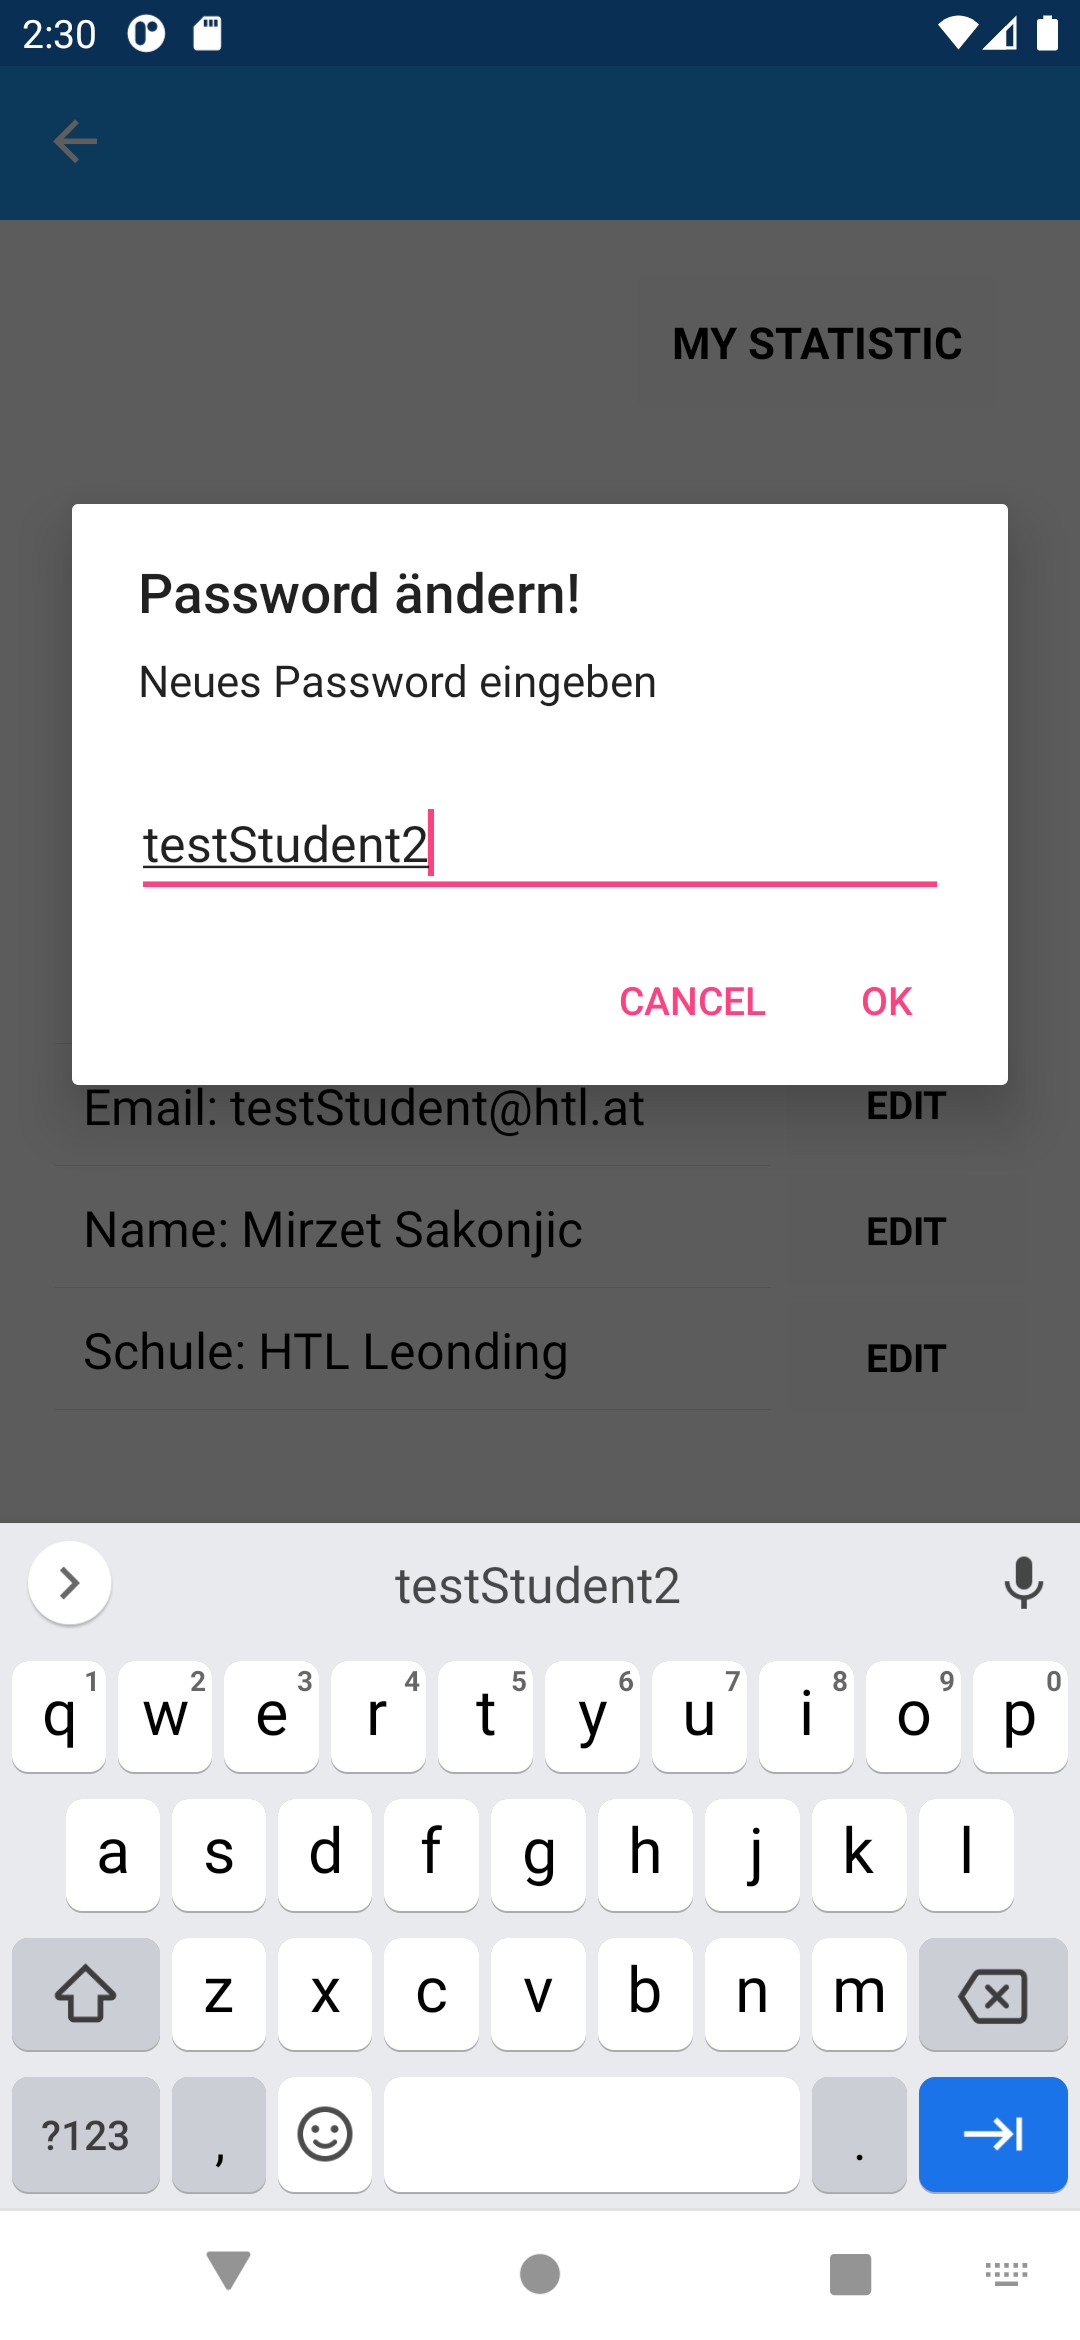
\includegraphics[width=3cm]{pics/Xamarin Student/21.png}\hfill
    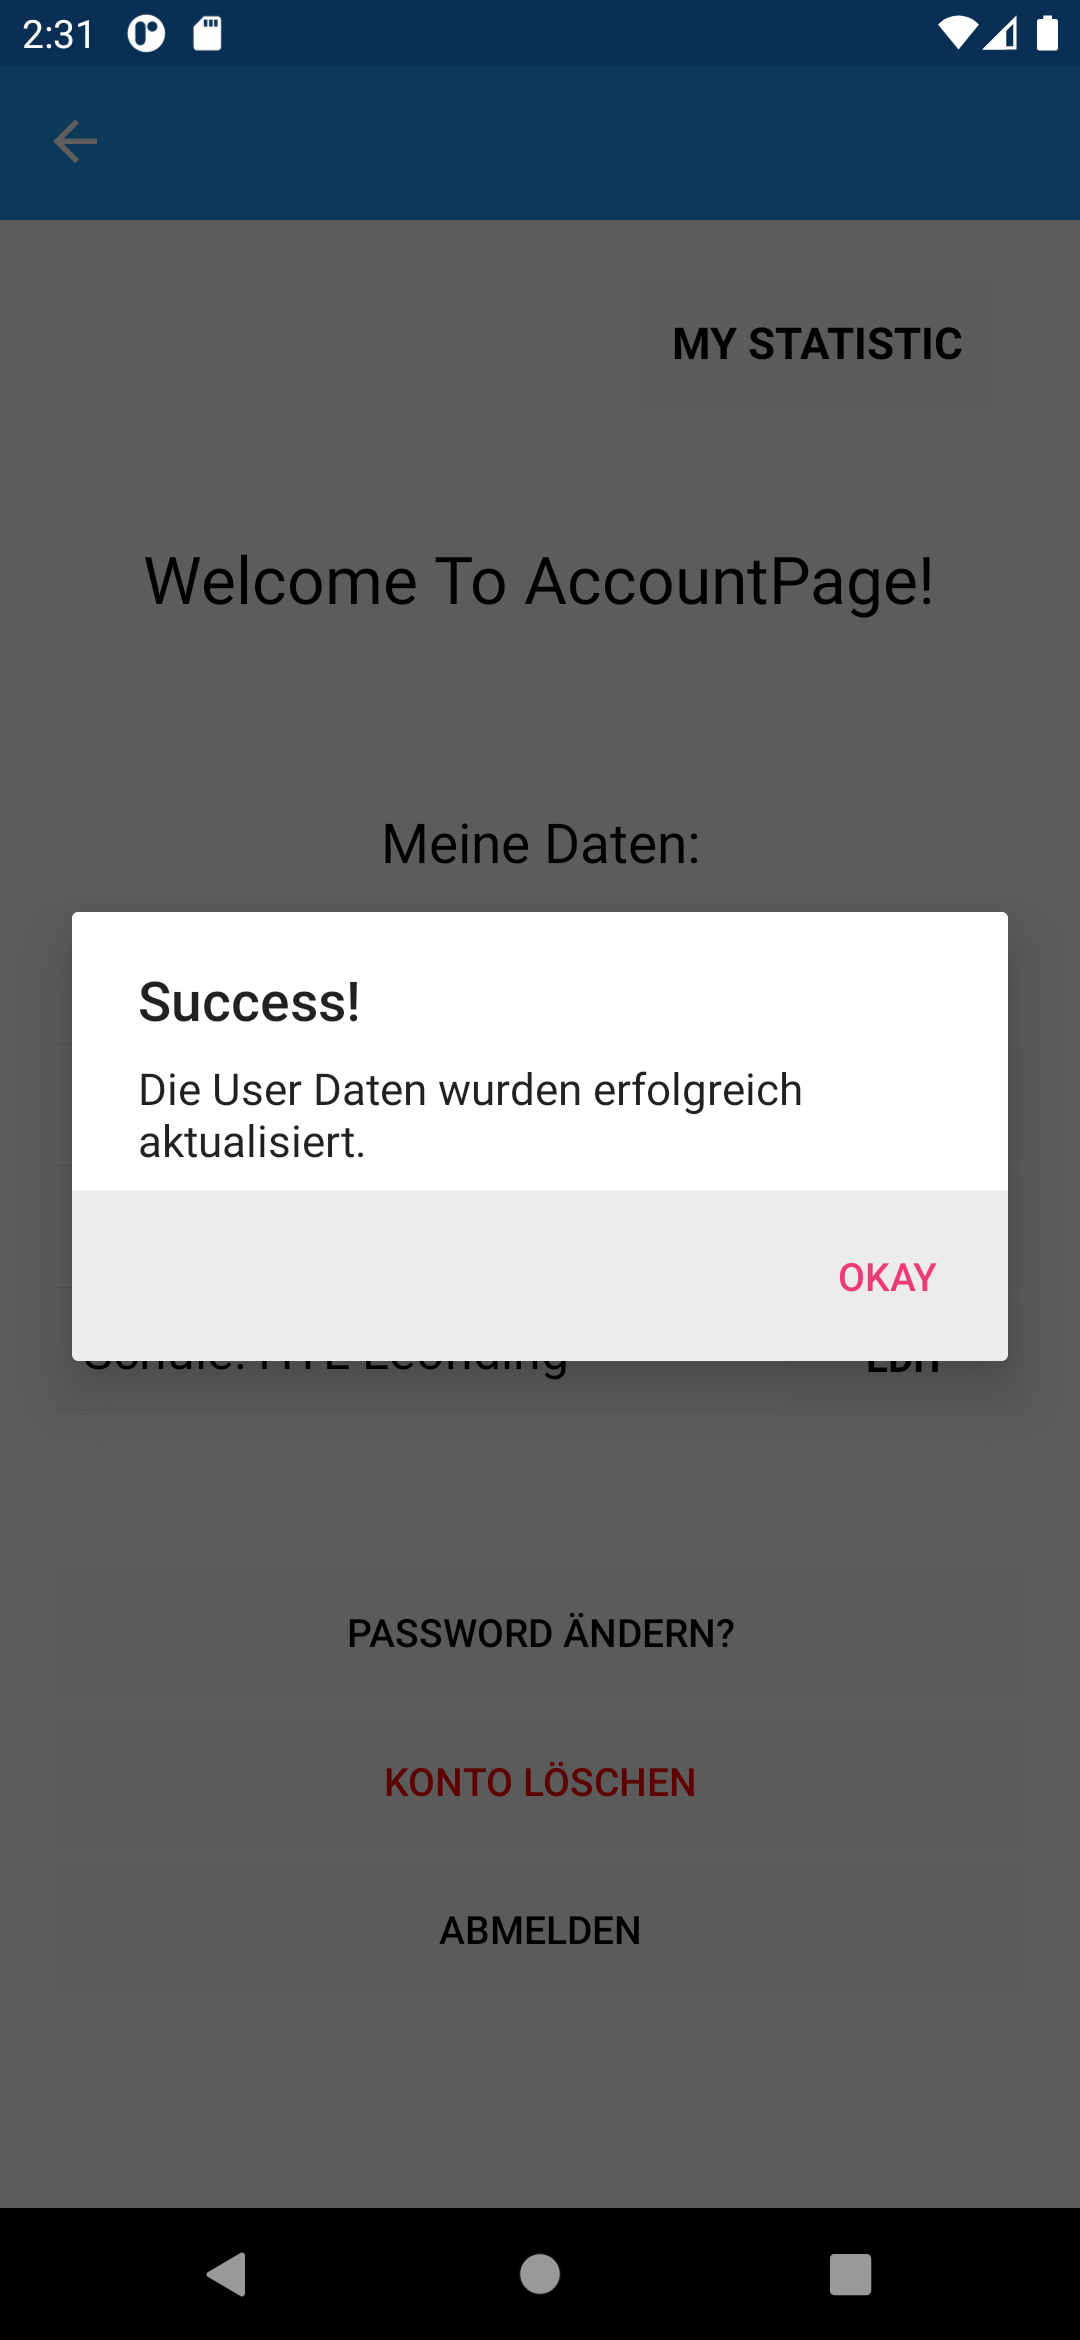
\includegraphics[width=3cm]{pics/Xamarin Student/22.png}
    \caption[MyAccount]{Passwort ändern}
    \end{center}
\end{figure}
\newpage
Das Löschen des Kontos ist durch Eingabe eines Passworts möglich, und alle Kontodaten werden entfernt und gelöscht.
\begin{figure}[h]
    \begin{center}
        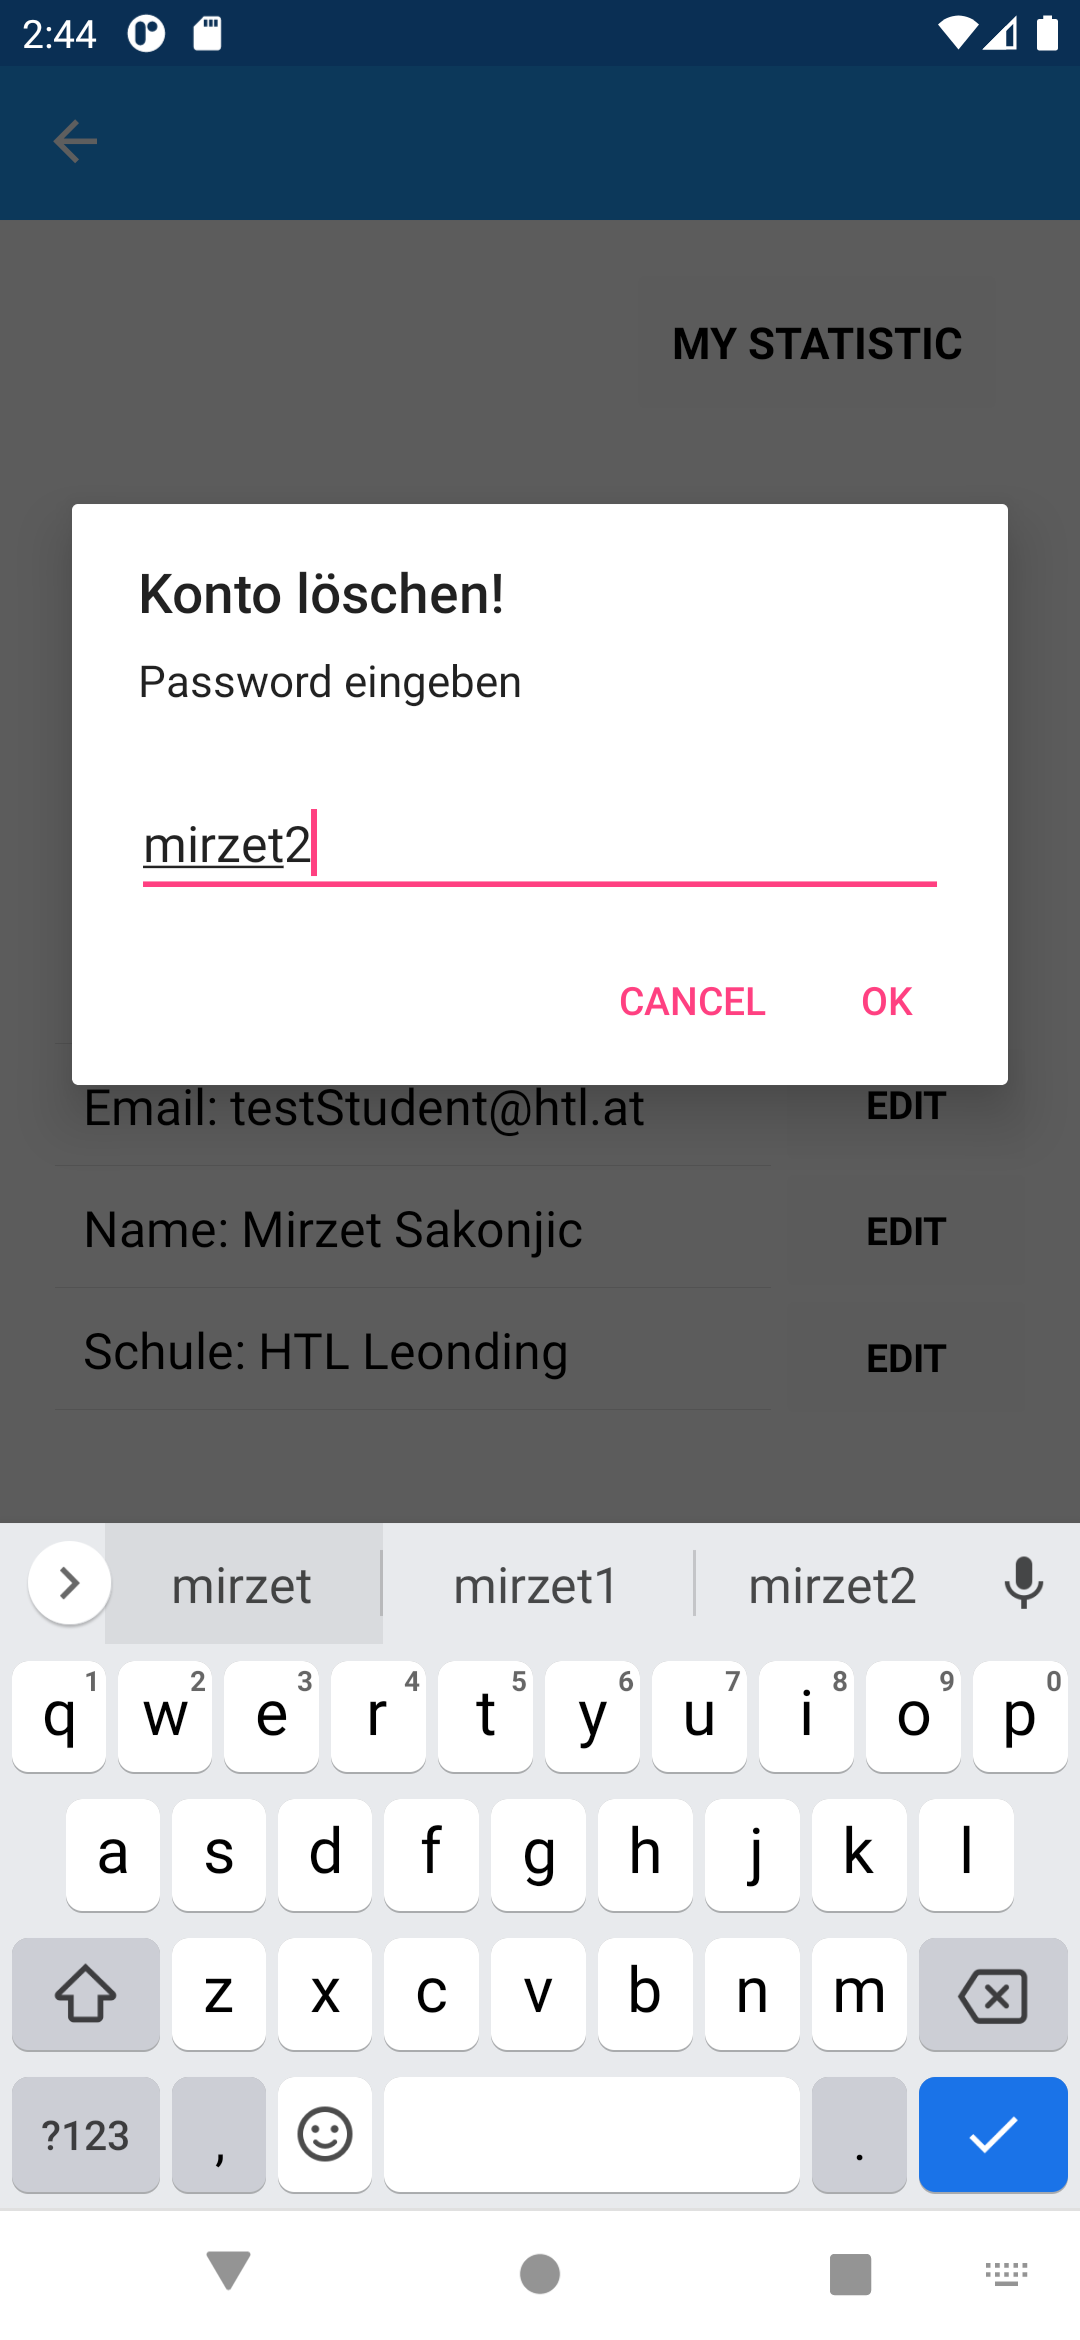
\includegraphics[width=3cm]{pics/Xamarin Student/23 Delete Acc Error.png}\hfill
        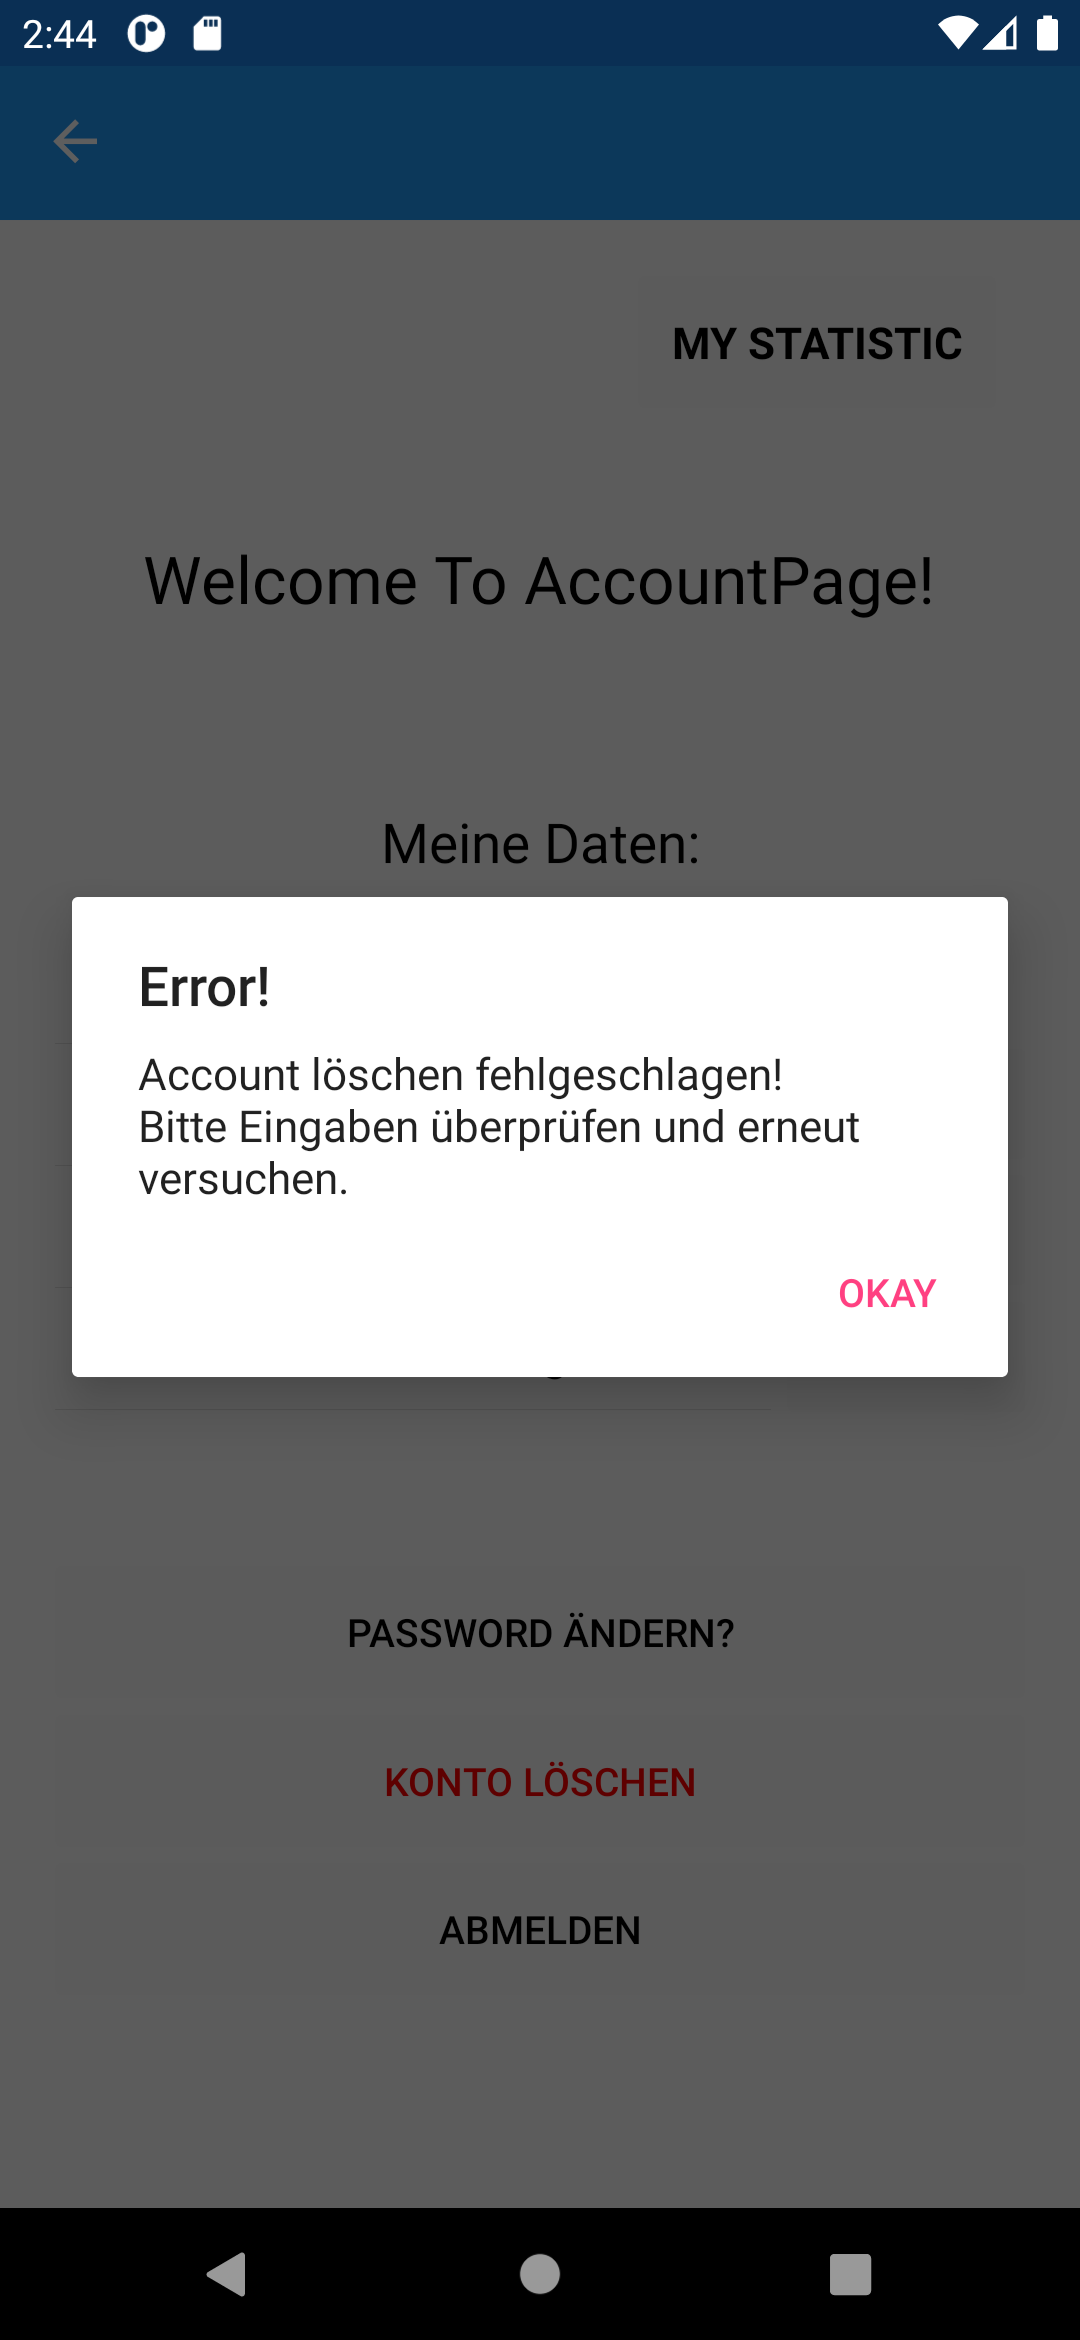
\includegraphics[width=3cm]{pics/Xamarin Student/24 Delete Acc Error.png}\hfill
        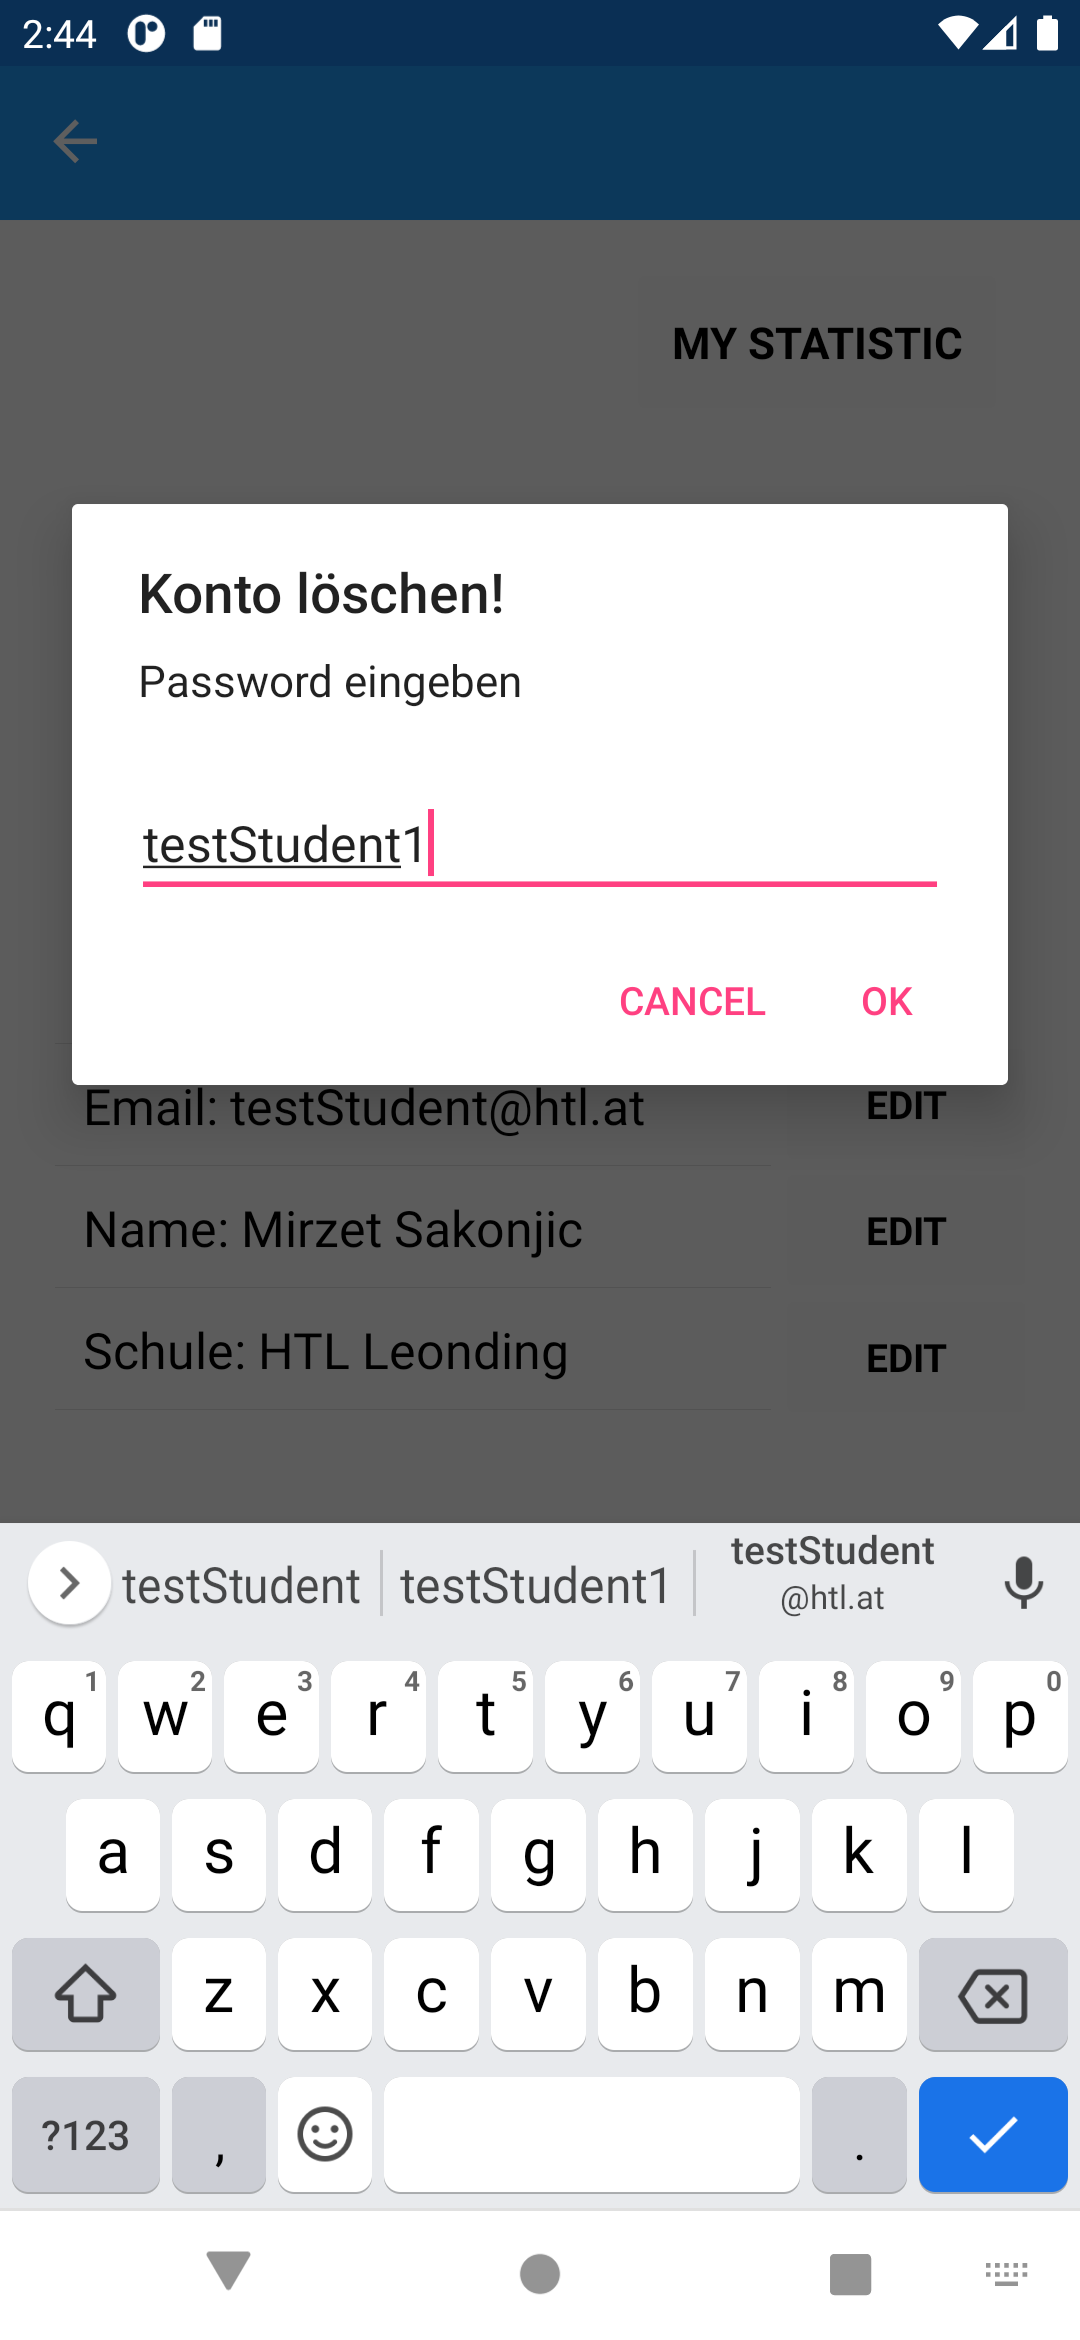
\includegraphics[width=3cm]{pics/Xamarin Student/25 Acc delete pass.png}\hfill
        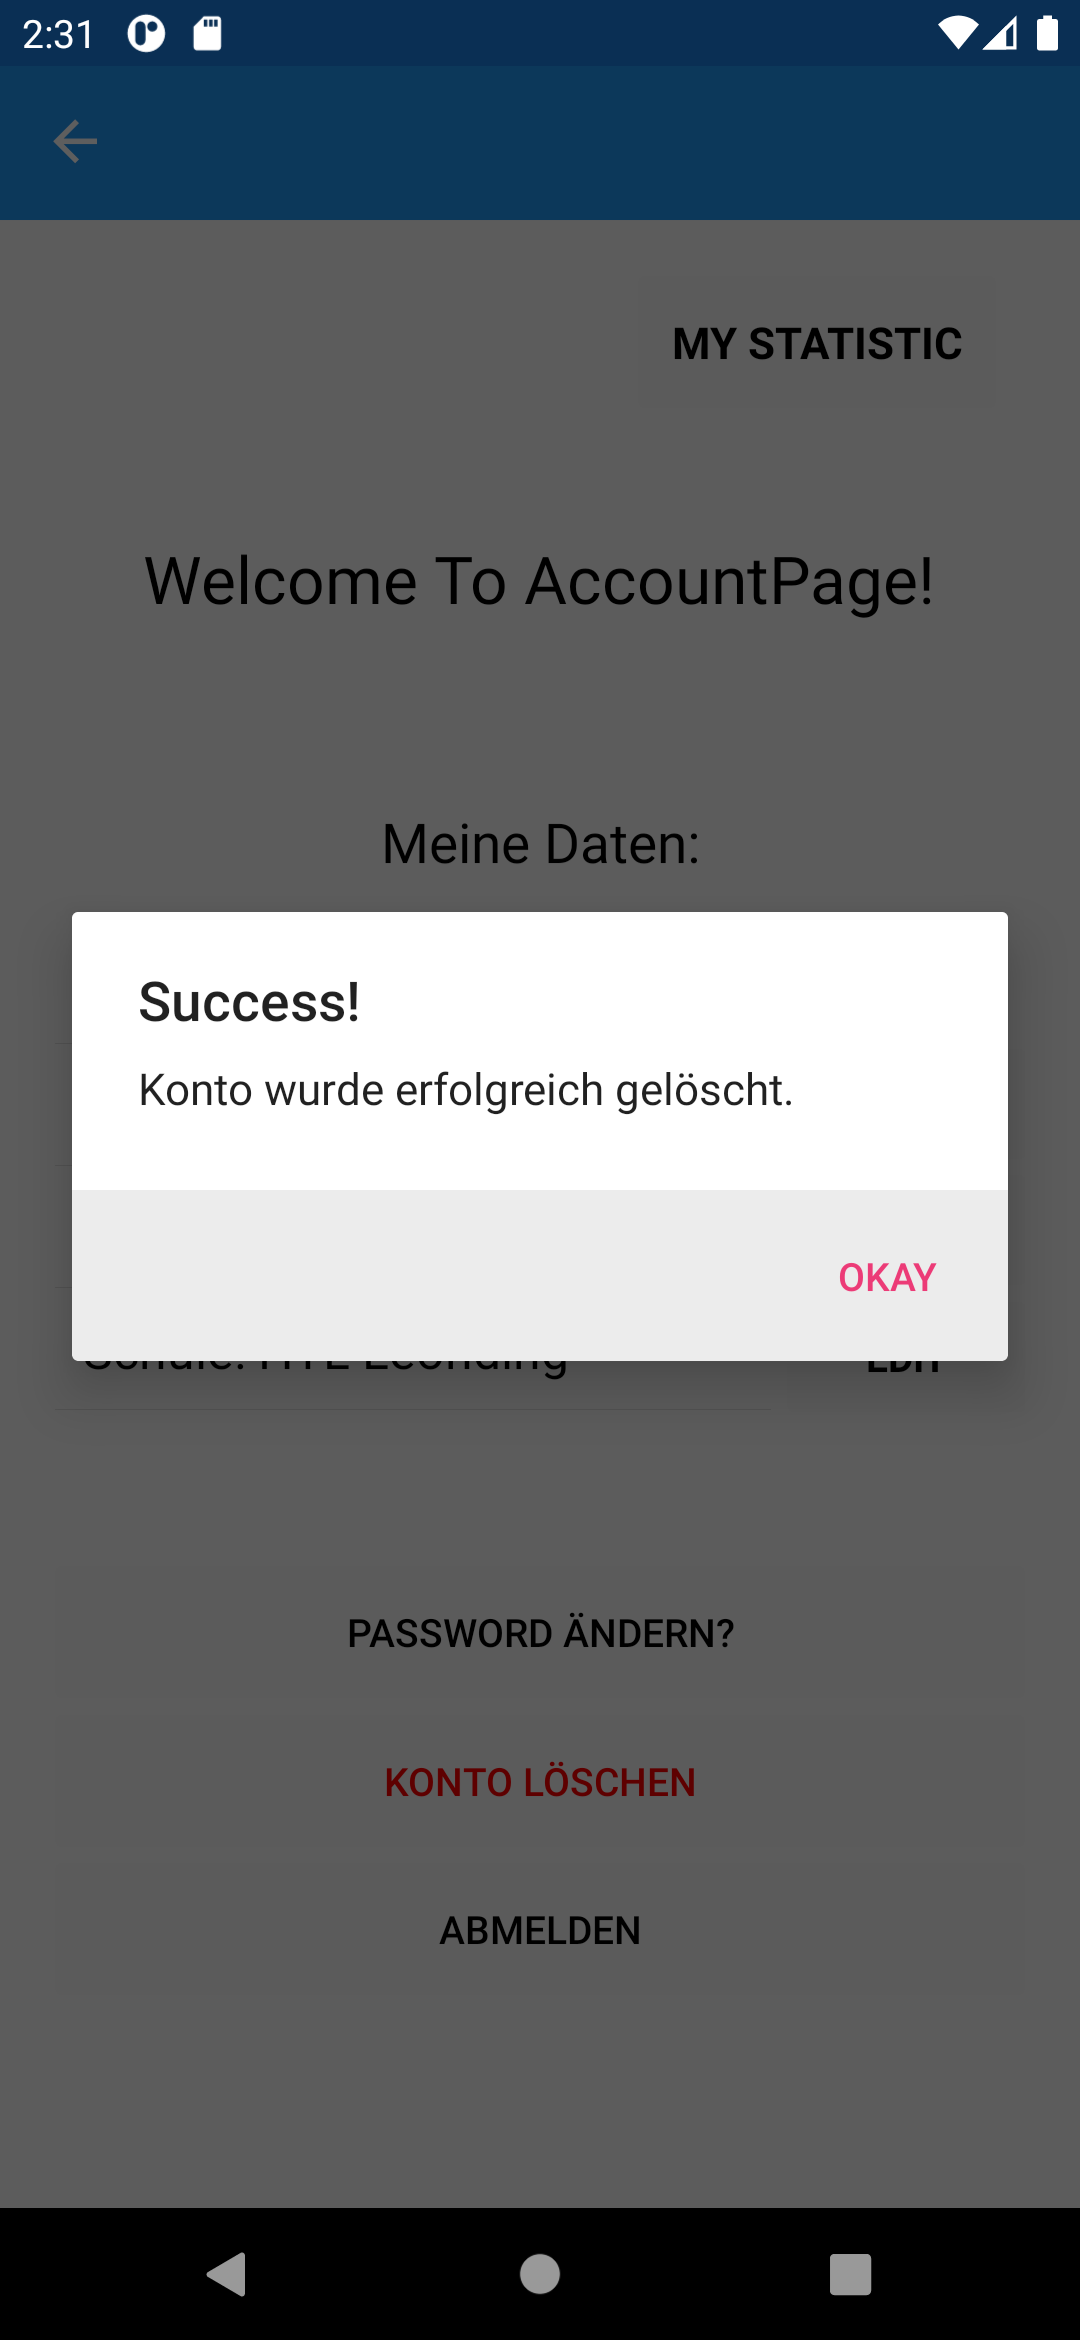
\includegraphics[width=3cm]{pics/Xamarin Student/23 Delete Acc.png}
        \caption[MyAccount]{Konto löschen}
        \end{center}
\end{figure}
\newline
Um sich abzumelden, müssen wir den Abmelden-Button drücken, und wir werden direkt auf die Login-Startseite zurückgeleitet.
\newline
Der einzige Unterschied auf der Benutzerkontoseite zwischen Schülern und Lehrern ist die Statistik in Button. So zeigt es für jeden Benutzer unterschiedliche Statistiken, zB wie viele Fächer der Lehrer eingegeben hat oder wie viel Feedback der Schüler gegeben hat.
\newpage

\section{Statistiken}
\subsection{Schüler}
Die Studentenstatistik wird in die Menge und Anzahl der abgegebenen Feedbacks eingerechnet. Das Messgerät zählt also alle Rückmeldungen und wirft eine Zahl als Summe aus.
\begin{figure}[h]
    \begin{center}
        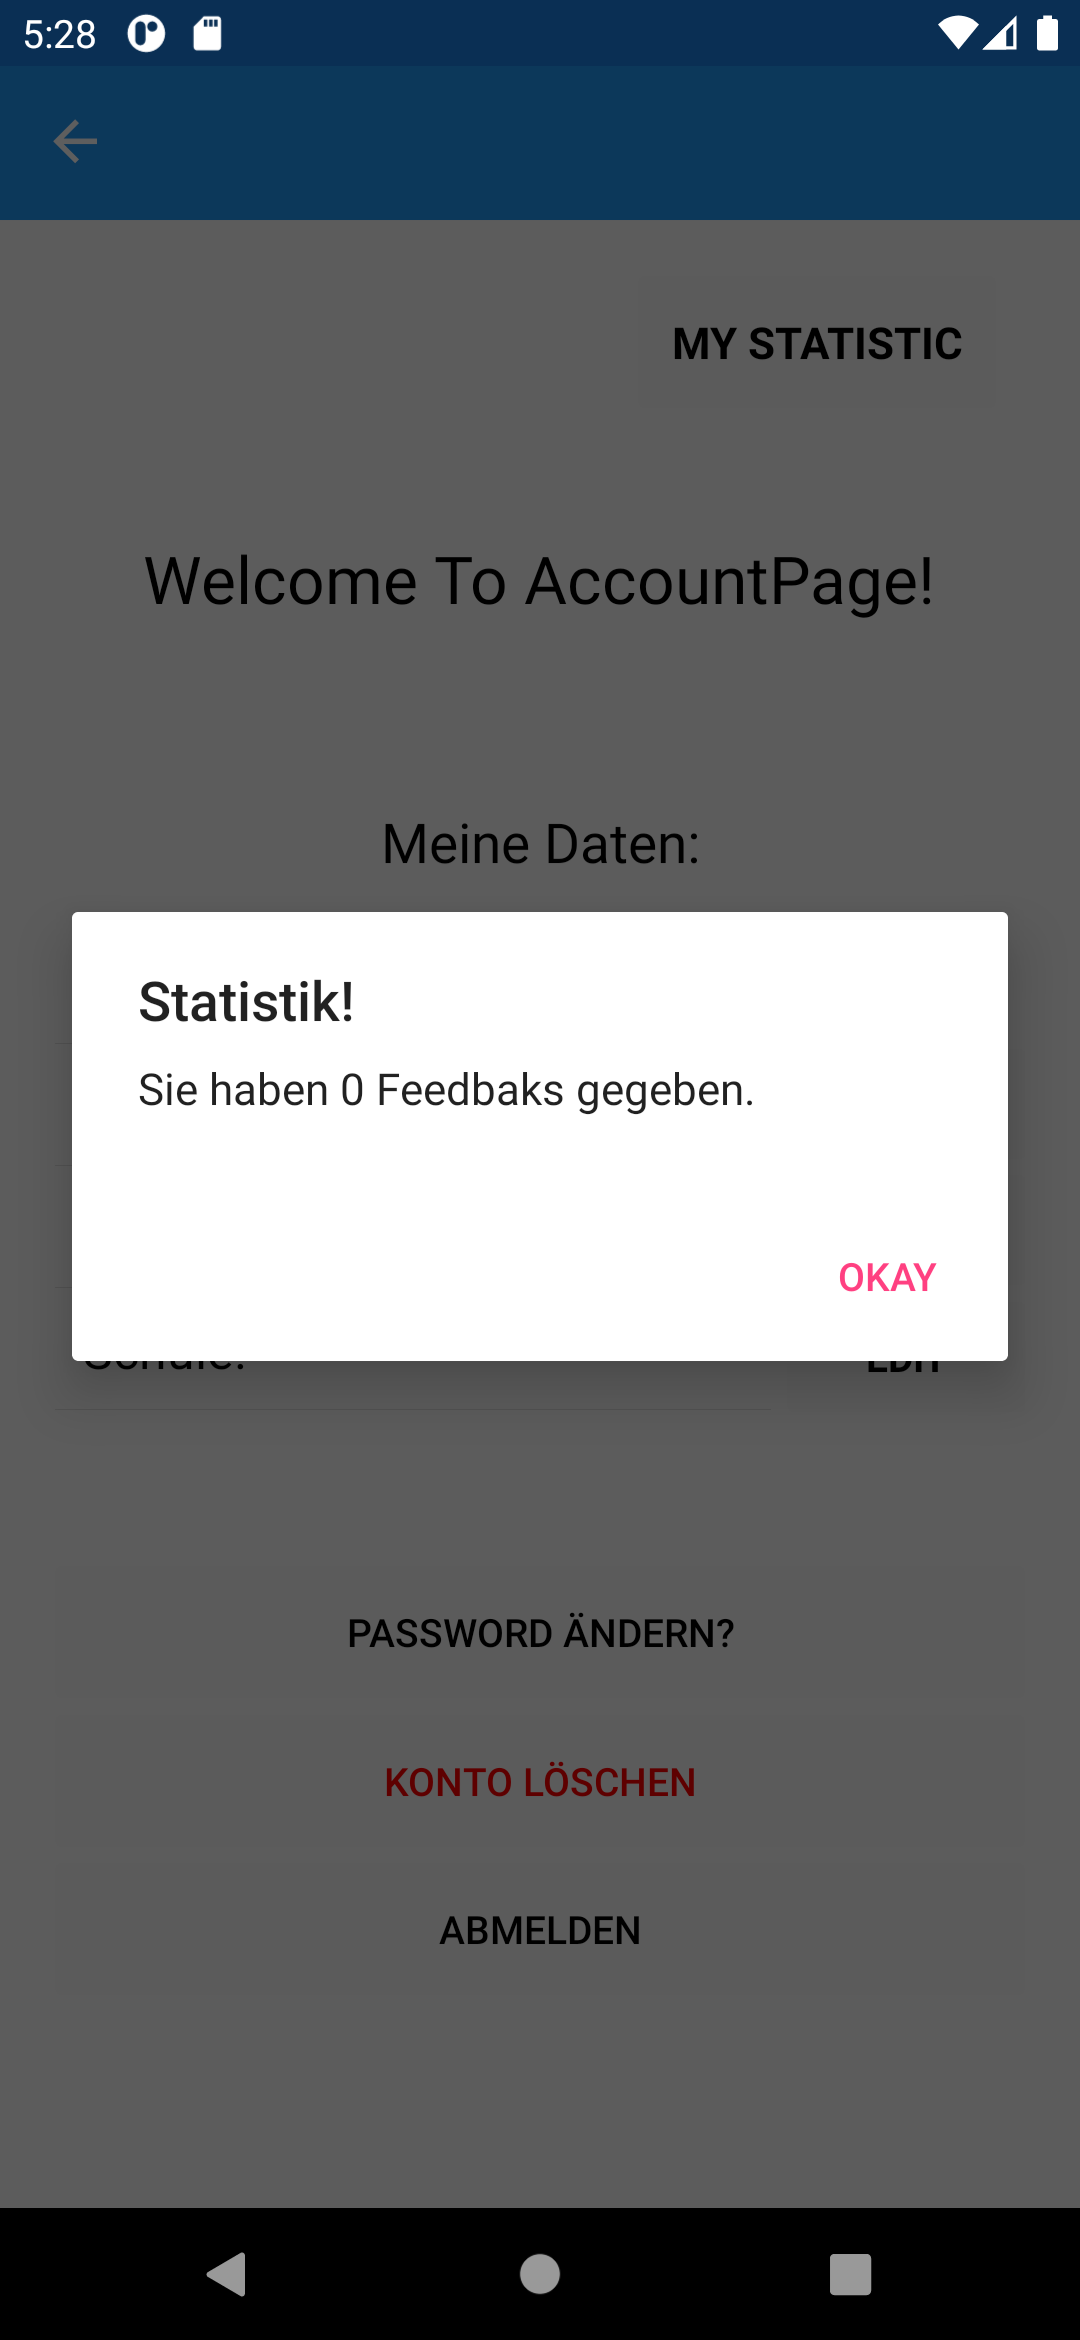
\includegraphics[width=4cm]{pics/Xamarin Student/27 Stat.png}\hfill
        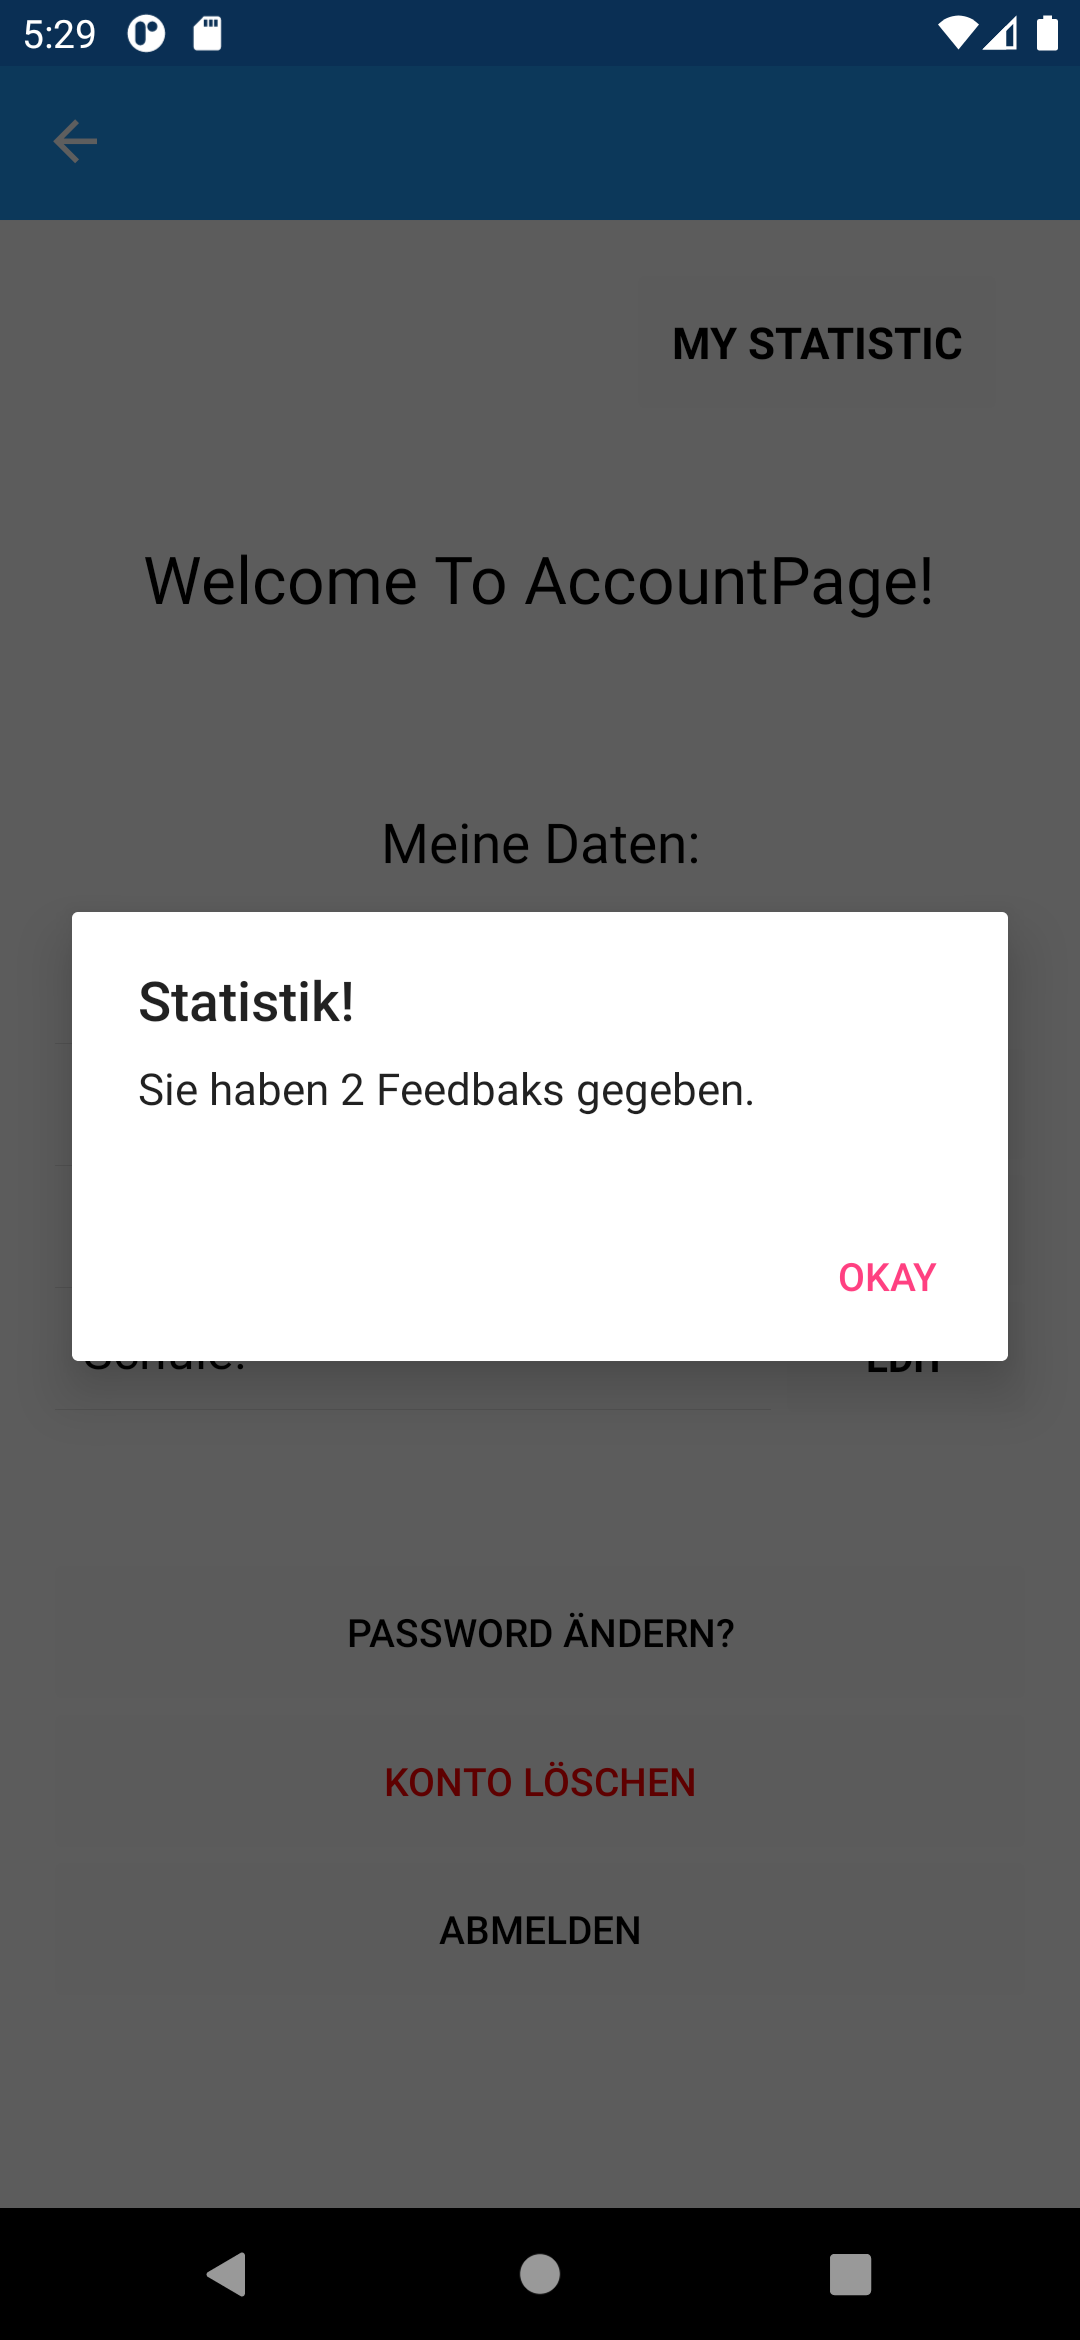
\includegraphics[width=4cm]{pics/Xamarin Student/28 Stat.png}
        \caption[Statistiken]{Statistiken Schüler}
        \end{center}
\end{figure}
\newpage
\subsection{Lehrer}
Die Lehrerstatistik wird in der Menge und Anzahl der abgegebenen Feedbacks gezählt. Es zeigt zusätzlich die durchschnittliche Bewertung aller Feddbacks (AVG).
\begin{figure}[h]
    \begin{center}
        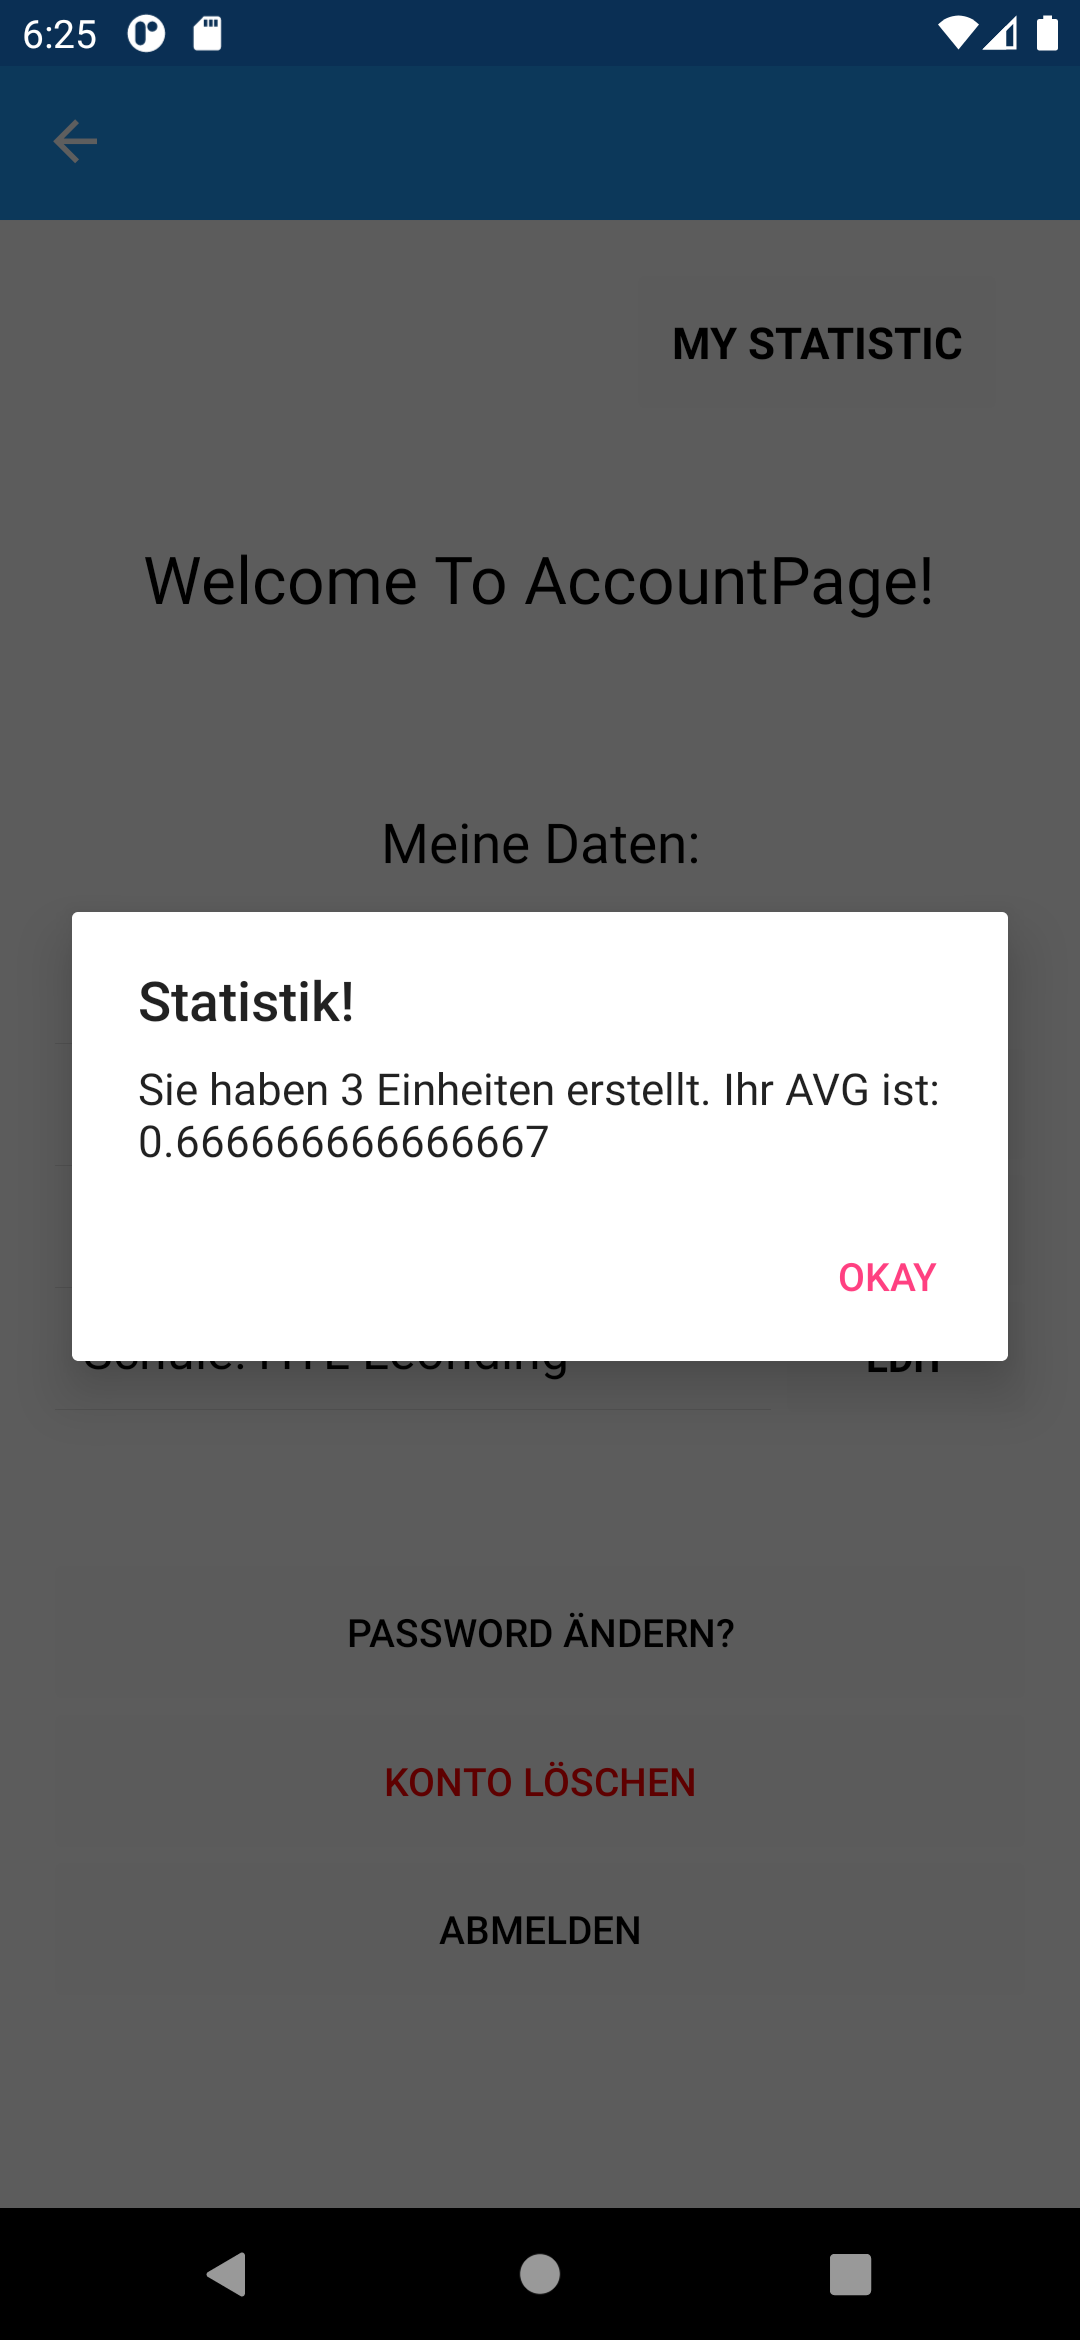
\includegraphics[width=4cm]{pics/Xamarin Lehrer/1 Stat.png}\hfill
        \caption[Statistiken]{Statistiken Lehrer}
        \end{center}
\end{figure}
\newpage

\begin{spacing}{1}
\chapter{Umsetzung}\label{chapter:implementation}
\end{spacing}
\section{Backend}
\author{Stefano Pyringer}

\subsection{Datenbank}
\author{Stefano Pyringer}

\newpage

\subsection{Web API}
\author{Stefano Pyringer}

\subsubsection{Benutzerverwaltung}
\author{Stefano Pyringer}

\begin{figure}[h]
    \includegraphics*[width=15cm]{./pics/Screenshot_Swagger_Auth.png}
    \caption[Swagger Benutzerverwaltung]{Screenshot Swagger Web API Dokumentation Benutzerverwaltung}
\end{figure}

Für das Usermanagement wird das NuGet Package ASP NET Identity verwendet. Der Authenticate-Controller ermöglicht die Registrierung, den Login und die Löschung des Benutzerkontos. 
Zusätzlich kann das Passwort und die E-Mail Adresse nachträglich geändert werden. Schüler und Lehrende werden durch Rollen getrennt.
Bei erfolgreicher Authentifizierung wird ein gültiger JSON Web Token zurückgesendet. 

Der Benutzername muss folgende Kriterien erfüllen:
\begin{itemize}
    \item mindestens 6 Zeichen
    \item maximal 26 Zeichen
    \item keine Leerzeichen
    \item keine Sonderzeichen (Umlaute sind erlaubt)
\end{itemize}

Das Passwort hat folgende Mindestanforderungen:
\begin{itemize}
    \item mindestens 6 Zeichen
    \item keine Leerzeichen
    \item mindestens einen Großbuchstaben, einen Kleinbuchstaben und eine Zahl
\end{itemize}

Diese Anforderungen sind in der Start-Up Konfiguration der ASP NET Core Web API festgelegt und werden zusätzlich von 
der Klasse AuthenticateValidations.cs kontrolliert. Im Fehlerfall wird ein entsprechender HTTP-Fehlercode zurückgegeben.

Der UserAccount-Controller ermöglicht das Hinzufügen folgender Daten:
\begin{itemize}
    \item Titel
    \item Vorname
    \item Nachname
    \item Geburtsdatum
    \item Lehranstalt
\end{itemize}

\begin{figure}[h]
    \includegraphics*[width=15cm]{./pics/screenshot_Startup_PwUserReq.png}
    \caption[PW User Requirements Startup]{Screenshot Startup.cs Benutzername und Passwort Anforderungen}
\end{figure}

\newpage
\subsubsection{Authentifizierung}
\author{Stefano Pyringer}
Die Login-Methode sendet ein HTTP OK Response mit dem gültigen JWT Token als Objekt zurück. 
Der Token ist 15 Minuten lang gültig und beinhaltet die Id des Benutzerkontos und deren Rolle. 
Dieser erlaubt es, je nach Rolle, Zugriff auf die geschützten Bereiche der Web API.

\begin{figure}[h]
    \includegraphics*[width=15cm]{./pics/screenshot_jwt_create.png}
    \caption[JWT create]{Screenshot JWT Token Erstellung detailiert}
\end{figure}

\newpage
\section{Frontend}
\author{Mirzet Sakonjic}
\subsection*{Login}
Die Anwendungsseite wird ausschließlich in der Oberfläche realisiert, 
indem das Bild in einem separaten Ressourcenordner gespeichert und mit <img> 
angezeigt wird. Das Bild auf der Startseite ist urheberrechtlich geschützt, 
da sich dieses eine Bild nur auf der Anmeldeseite befindet. Beim Einloggen gibt 
der Nutzer seine E-Mail-Adresse und sein Passwort ein, die bereits ausgelesen 
und im Hintergrund in der Datenbank gespeichert wurden. Bei Bedarf kann ein 
neuer Benutzer angelegt werden. Die Validierung überprüft, ob die E-Mail-Adresse 
und das Passwort eingegeben wurden. Es überprüft auch Passwortregeln wie Länge, 
Großbuchstaben oder zusätzliche Zeichen.
Wenn der User auf den Button „Login“ drückt, wird ein API Get-Request mit der
eingegebenen E-Mail und Passwort ans Backend gesendet. Wenn die Zugangsdaten
stimmen und der User vorhanden ist, werden die Logindaten inklusive Username
zurückgesendet und in der globalen Komponente abgespeichert, damit im gesamten
Projekt darauf zugegriffen werden kann.
Sollten die Zugangsdaten nicht stimmen, wird eine Fehlermeldung angezeigt.
Nach dem erfolgreichen Laden aller Daten wird der User zu der Startseite
weitergeleitet.

\subsection*{Benutzerkontoverwaltung}

\begin{spacing}{1}
\chapter{Nicht realisierte Funktionen}\label{chapter:not_implemented_f}
\end{spacing}
Aufgrund von diversen Schwierigkeiten, die wir während der Diplomarbeit konfrontiert waren, konnten einige 
Funktionen der App nicht rechtzeitig implementiert werden.

\section{Feedback Kategorien}
\author{Stefano Pyringer}
Der Lehrende hätte bei der Erstellung bei der Lehreinheit, eigene Kategorien mit Sternen oder Kommentar anlegen können, 
um ein präziseres Feedback von den Schülern erhalten zu können. 

\section{Export als PDF}
\author{Stefano Pyringer}
Diese Funktion sollte den Ausdruck und externe Speicherung von Statistiken, Lehreinheiten und deren Bewertungen vereinfachen.

\section{digitale Erfolge/Abzeichen}
\author{Stefano Pyringer}
Bei dieser Idee wurde die PC-Spiele Plattform Steam als Vorbild genommen, die gewisse Erfolge mittels Abzeichen die im Benutzerprofil öffentlich
sichtbar gemacht werden können, um die Motivation für gewisse nicht verpflichtende Tätigkeiten im Spiel zu steigern. 
Dies sollte in der Feedback App ebenfalls möglich gemacht werden. Zudem kann der Lehrende auch sehen, ob der Bewerter aufgrund bestimmter Erfolgsabzeichen eventuell mehr Erfahrung 
mit dem Feedback geben hat und somit die Bewertung ehrlicher und eine mehr konstruierte Rückmeldung gegenüber anderen hat.

\section{Benachrichtigungen}
\author{Stefano Pyringer}
Auf den mobilen Endgerät sollte der Benutzer mittels benachrichtigt werden, wenn er Feedback von anderen Benutzern erhalten hat oder seine 
Lehreinheit das Ablaufdatum erreicht hat. Zudem war eine Benachrichtigung mittel E-Mail geplant.

\section{Two-Faktor Authentifizierung}
\author{Stefano Pyringer}
Der Benutzer hätte entscheiden können, ob er die sichere 2-Faktor Anmeldemethode verwendet. Dabei handelt es sich um eine 
Eingabe eines zweiten Kennworts, dass automatisch von einem externen Dienst wie Google Authenticator erstellt wurde. 
Dieser Pin ist zeitlich begrenzt und erhöht damit erheblich die Sicherheit, um den Missbrauch eines Accounts zu verhindern.

\section{Benutzerkonto Profilfoto}
\author{Stefano Pyringer}
Die Hinzufügung eines Profilbilds hätte der User sein Benutzerkonto individueller gestalten können. Diese Bild wäre in einem 
platzsparenden Format (JPEG) mit Höhen- und Längenbegrenzung auf dem Server mit der Feedback Datenbank in der Tabelle User hochgeladen worden.


\begin{spacing}{1}
\chapter{Zusammenfassung}
\end{spacing}
Aufzählungen:

\begin{compactitem}
    \item Itemize Level 1
    \begin{compactitem}
        \item Itemize Level 2
        \begin{compactitem}
            \item Itemize Level 3 (vermeiden)
        \end{compactitem}
    \end{compactitem}
\end{compactitem}

\begin{compactenum}
    \item Enumerate Level 1
    \begin{compactenum}
        \item Enumerate Level 2
        \begin{compactenum}
            \item Enumerate Level 3 (vermeiden)
        \end{compactenum}
    \end{compactenum}
\end{compactenum}

\begin{compactdesc}
    \item[Desc] Level 1
    \begin{compactdesc}
        \item[Desc] Level 2 (vermeiden)
        \begin{compactdesc}
            \item[Desc] Level 3 (vermeiden)
        \end{compactdesc}
    \end{compactdesc}
\end{compactdesc}

\newpage
\pagenumbering{Roman}
\setcounter{page}{\value{RPages}}
\newacronym{guid}{GUID}{Globally Unique Identifier}
\newacronym{jit}{JIT}{Just In Time Compiler}
\newacronym{nfc}{NFC}{Near Field Communication}
\newacronym{rfid}{RFID}{Radio Frequency Identification}

% Usage:
% \gls{label} lowercase in text
% \Gls{label} Uppercase in text
% \newacronym{label}{abbrev}{full}
% \newglossaryentry{label}{settings}



%\setlength{\glsdescwidth}{0.8\linewidth}
\glsnogroupskiptrue
\printglossary[title=Glossar,toctitle=Glossar] %,style=long]
\spacing{1}{
%\bibliographystyle{IEEEtran}
\bibliographystyle{ieeetrande}
\bibliography{bib}
}
\listoffigures
\listoftables
\lstlistoflistings
\appendix
\addchap{Anhang}
\input{./sections/appendix}
\end{document}

